\documentclass[11pt]{fsuthesis}

\usepackage{textcase}
\usepackage[pdftex]{graphicx}
%\usepackage{hyperref}
%\hypersetup{breaklinks=true}


% Added packages
\usepackage[usenames]{color}
\usepackage{amsfonts, amsmath, amssymb, graphics}

% NOTE: bibentry MUST appear before the hyperref or build will fail
\usepackage{bibentry}
\nobibliography*

\usepackage[
    hyperindex=true,		% Make numbers of index links as well
   	backref=page, 		% Provide page listing where refs occur in the bibliography
	%breaklinks=true,
    colorlinks,%
    citecolor=green,%
    filecolor=blue,%
    linkcolor=red,%
    urlcolor=red, 
]{hyperref}

\usepackage{dsfont}

\title{Multi-GPU Solutions of Geophysical PDEs with Radial Basis Function-generated Finite Differences}
\author{Evan F. Bollig}
\college{College of Arty Science}
\department{Department of Scientific Computing} % Delete if no department
\manuscripttype{Dissertation}                    % [Thesis, Dissertation, Treatise]
\degree{Doctor of Philosophy}                 
\semester{Fall}                          % [Spring, Summer, Fall]
\degreeyear{2012}
\defensedate{October 1, 2012}
%\subject{My Topic}
%\keywords{keyterm1; keyterm2; keyterm3; ...}

\committeeperson{Gordon Erlebacher}{Professor Directing Thesis}
\committeeperson{Natasha Flyer}{Professor Directing Thesis}
\committeeperson{Mark Sussman}{University Representative}
\committeeperson{Dennis Slice}{Committee Member}
\committeeperson{Ming Ye}{Committee Member}

%%%% USEPACKAGES for MACROS %%%%%
\usepackage{algpseudocode}
\usepackage[chapter]{algorithm}
\usepackage{caption}
\usepackage{subcaption}
\usepackage{url}

\usepackage{array}
\usepackage{arydshln}
\usepackage{multirow}
\usepackage{multicol}

\newcommand{\toprule}[0]{\hline}
\newcommand{\midrule}[0]{\hline\hline}
\newcommand{\bottomrule}[0]{\hline}

\DeclareSymbolFont{AMSb}{U}{msb}{m}{n}
\DeclareMathSymbol{\N}{\mathbin}{AMSb}{"4E}
\DeclareMathSymbol{\Z}{\mathbin}{AMSb}{"5A}
\DeclareMathSymbol{\R}{\mathbin}{AMSb}{"52}
\DeclareMathSymbol{\Q}{\mathbin}{AMSb}{"51}
\DeclareMathSymbol{\PP}{\mathbin}{AMSb}{"50}
\DeclareMathSymbol{\I}{\mathbin}{AMSb}{"49}
%\DeclareMathSymbol{\C}{\mathbin}{AMSb}{"43}

%%%%%% VECTOR NORM: %%%%%%%
\newcommand{\vectornorm}[1]{\left|\left|#1\right|\right|}
\newcommand{\vnorm}[1]{\left|\left|#1\right|\right|}
\newcommand{\by}[0]{\times}
\newcommand{\vect}[1]{\mathbf{#1}}
%\newcommand{\mat}[1]{\mathbf{#1}} 

%\renewcommand{\vec}[1]{ \textbf{#1} }
%%%%%%%%%%%%%%%%%%%%%%

%%%%%%% THM, COR, DEF %%%%%%%
%\newtheorem{theorem}{Theorem}[section]
%\newtheorem{lemma}[theorem]{Lemma}
%\newtheorem{proposition}[theorem]{Proposition}
%\newtheorem{corollary}[theorem]{Corollary}
%\newenvironment{proof}[1][Proof]{\begin{trivlist}
%\item[\hskip \labelsep {\bfseries #1}]}{\end{trivlist}}
%\newenvironment{definition}[1][Definition]{\begin{trivlist}
%\item[\hskip \labelsep {\bfseries #1}]}{\end{trivlist}}
%\newenvironment{example}[1][Example]{\begin{trivlist}
%\item[\hskip \labelsep {\bfseries #1}]}{\end{trivlist}}
%\newenvironment{remark}[1][Remark]{\begin{trivlist}
%\item[\hskip \labelsep {\bfseries #1}]}{\end{trivlist}}
%\newcommand{\qed}{\nobreak \ifvmode \relax \else
%      \ifdim\lastskip<1.5em \hskip-\lastskip
%      \hskip1.5em plus0em minus0.5em \fi \nobreak
%      \vrule height0.75em width0.5em depth0.25em\fi}
%%%%%%%%%%%%%%%%%%%%%%


% \DeclareMathOperator{\Sample}{Sample}
%\let\vaccent=\v % rename builtin command \v{} to \vaccent{}
%\renewcommand{\vec}[1]{\ensuremath{\mathbf{#1}}} % for vectors
\newcommand{\gv}[1]{\ensuremath{\mbox{\boldmath$ #1 $}}} 
% for vectors of Greek letters
\newcommand{\uv}[1]{\ensuremath{\mathbf{\hat{#1}}}} % for unit vector
\newcommand{\abs}[1]{\left| #1 \right|} % for absolute value
\newcommand{\avg}[1]{\left< #1 \right>} % for average
\let\underdot=\d % rename builtin command \d{} to \underdot{}
\renewcommand{\d}[2]{\frac{d #1}{d #2}} % for derivatives
\newcommand{\dd}[2]{\frac{d^2 #1}{d #2^2}} % for double derivatives
\newcommand{\pd}[2]{\frac{\partial #1}{\partial #2}} 
% for partial derivatives
\newcommand{\pdd}[2]{\frac{\partial^2 #1}{\partial #2^2}} 
\newcommand{\pdda}[3]{\frac{\partial^2 #1}{\partial #2 \partial #3}} 
% for double partial derivatives
\newcommand{\pdc}[3]{\left( \frac{\partial #1}{\partial #2}
 \right)_{#3}} % for thermodynamic partial derivatives
\newcommand{\ket}[1]{\left| #1 \right>} % for Dirac bras
\newcommand{\bra}[1]{\left< #1 \right|} % for Dirac kets
\newcommand{\braket}[2]{\left< #1 \vphantom{#2} \right|
 \left. #2 \vphantom{#1} \right>} % for Dirac brackets
\newcommand{\matrixel}[3]{\left< #1 \vphantom{#2#3} \right|
 #2 \left| #3 \vphantom{#1#2} \right>} % for Dirac matrix elements
\newcommand{\grad}[1]{\gv{\nabla} #1} % for gradient
\let\divsymb=\div % rename builtin command \div to \divsymb
\renewcommand{\div}[1]{\gv{\nabla} \cdot #1} % for divergence
\newcommand{\curl}[1]{\gv{\nabla} \times #1} % for curl
\let\baraccent=\= % rename builtin command \= to \baraccent
\renewcommand{\=}[1]{\stackrel{#1}{=}} % for putting numbers above =
\newcommand{\diffop}[1]{\mathcal{L}#1}
\newcommand{\boundop}[1]{\mathcal{B}#1}
\newcommand{\rvec}[0]{{\bf r}}

\newcommand{\Interior}[0]{\Omega}
\newcommand{\domain}[0]{\Omega}
\newcommand{\Boundary}[0]{\partial \Omega}
%\newcommand{\Boundary}[0]{\Gamma}

\newcommand{\on}[1]{\hskip1.5em \textrm{ on } #1}

\newcommand{\gemm}{\texttt{GEMM}}
\newcommand{\trmm}{\texttt{TRMM}}
\newcommand{\gesvd}{\texttt{GESVD}}
\newcommand{\geqrf}{\texttt{GEQRF}}


\newcommand{\minitab}[2][l]{\begin{tabular}{#1}#2\end{tabular}}
\newcommand{\comm}[1]{\textcolor{red}{\textit{#1}}}

\newcommand{\nfrac}[2]{
\nicefrac{#1}{#2}
%\frac{#1}{#2}
}

\usepackage{xparse}


%%%%%%%%%%%%%%%
% Show a Author's Note
% USAGE: 
% \incomplete[Optional footnote message to further clarify note]{The text which is currently not finished}
\DeclareDocumentCommand \incomplete{ o m }
{%
\IfNoValueTF {#1}
{\textcolor{red}{Incomplete: \ul{#2}}} 
{\textcolor{red}{Incomplete: \ul{#2}}\footnote{Comment: #1}}%
}
%%%%%%%%%%%%%%%



%%%%%%%%%%%%%%%
% Show a Author's Note
% USAGE: 
% \authnote[Optional footnote message to further clarify note]{The note to your readers}
\DeclareDocumentCommand \authnote { o m }
{%
\IfNoValueTF {#1}
{\textcolor{blue}{Author's Note: \ul{#2}}} 
{\textcolor{blue}{Author's Note: \ul{#2}}\footnote{Comment: #1}}%
}
%%%%%%%%%%%%%%%



%%%%%%%%%%%%%%%
% Strike out text that doesn't belong in the paper
% USAGE: 
% \strike[Optional footnote to state why it doesn't belong]{Text to strike out}
\DeclareDocumentCommand \strike { o m }
{%
\setstcolor{red}
\IfNoValueTF {#1}
{\textcolor{Gray}{\st{#2}}} 
{\textcolor{Gray}{\st{#2}}\footnote{Comment: #1}}%
}
%%%%%%%%%%%%%%%




% colors to show the corrections
\newcommand{\red}[1]{\textbf{\textcolor{red}{#1}}}
\newcommand{\blue}[1]{\textbf{\textcolor{blue}{#1}}}
\newcommand{\cyan}[1]{\textbf{\textcolor{cyan}{#1}}}
\newcommand{\green}[1]{\textbf{\textcolor{green}{#1}}}
\newcommand{\magenta}[1]{\textbf{\textcolor{magenta}{#1}}}
\newcommand{\orange}[1]{\textbf{\textcolor{orange}{#1}}}
%%%%%%%%%% DK DK
% comments between authors
\newcommand{\toall}[1]{\textbf{\green{@@@ All: #1 @@@}}}
\newcommand{\toevan}[1]{\textbf{\red{*** Evan: #1 ***}}}
%\newcommand{\toevan}[1]{}  % USE FOR FINAL VERSION
\newcommand{\toe}[1]{\textbf{\red{*** Evan: #1 ***}}}
\newcommand{\tog}[1]{\textbf{\blue{*** Gordon: #1 ***}}}
%\newcommand{\togordon}[1]{\textbf{\blue{*** Gordon: #1 ***}}}
\renewcommand{\ge}[3]{{\textcolor{blue}{*** \textbf{Gordon:}\strike{#1} #2 ***}}\red{(#3)}}
\renewcommand{\ge}[3]{{\textcolor{blue}{#2}}}
\renewcommand{\ge}[3]{{\textcolor{red}{#2}}}
\newcommand{\eb}[3]{{\textcolor{red}{*** \textbf{Evan:}\strike{#1} #2 ***}}\red{(#3)}}
\renewcommand{\eb}[3]{{{\textcolor{red}{#2}}}}
%\def\ge#1#2#3{}{\textbf{\blue{*** Gordon: #2 ***}}}{(#3)}
\newcommand{\gee}[1]{{\bf{\blue{{\em #1}}}}}
\newcommand{\old}[1]{}
\newcommand{\del}[1]{***#1*** }



\input{macros/misc_mac.tex}
\newcommand{\mathsym}[1]{{}}
\newcommand{\unicode}[1]{{}}
\newcommand{\ep}{\epsilon}
\newcommand{\vx}{\mathbf{x}}


\usepackage{tabularx} 
\newcolumntype{C}{>{\centering\arraybackslash}b{1in}}
\newcolumntype{L}{>{\flushleft\arraybackslash}b{1.5in}}
\newcolumntype{R}{>{\flushright\arraybackslash}b{1.5in}}
\newcolumntype{D}{>{\flushright\arraybackslash}b{2.0in}}
\newcolumntype{E}{>{\flushright\arraybackslash}b{1.0in}}


 

\begin{document}

%% UNCOMMENT THIS FOR ETD CLEARANCE
\frontmatter
%\maketitle
%\makecommitteepage
%%
%
\begin{dedication}
This work is dedicated to the one who taught me patience, compassion, bravery, and determination. Thank you, Mom.
  
\begin{center}
\emph{--E}
\end{center}
\end{dedication}

%\begin{acknowledgments}

I feel compelled to start by thanking my major professor, Dr. Gordon Erlebacher, who shared with me a unique attitude and excitement in regard to research. After years of collaboration, I find myself echoing his own audacious style in questioning the work done by others; never quite satisfied by their responses. Without his supervision and constant prodding this dissertation would not have been possible. %Gordon's skill as a computational scientist is exemplary. Time and again I have watched him fearlessly work in areas outside his own domain of expertise in a way I can only hope to simulate. 

Of no lesser significance is Dr. Natasha Flyer, who is not formally listed as a co-advisor due to restrictions at the university level, but who has in all capacities fulfilled that role. I am sincerely grateful for the time spent at NCAR under her tutelage. In addition to fortifying my understanding of RBF methods and geophysical PDEs, Natasha shared a number of unforgettable life-lessons that reflect in my choice of employment and pursuit of happiness today. 

I also extend my deepest gratitude to the remainder of my committee for their patience and willingness to participate in this venture. 

In no particular order, I am indebted to:
\begin{itemize}
\item Leeia for being my best friend, biggest fan, and for supporting me through every trial and tribulation on the path to complete this work;
\item Drs. David Yuen, Bengt Fornberg, Grady Wright, John Burkardt and Kiran Katta for their support and feedback on numerical modeling;
\item the RBF research group at CU-Boulder for a number of ideas that led to interesting investigations;
\item Dr. Geoff Womeldorff for insightful discussion and the high resolution Spherical CVT meshes tested herein;
\item Steven Henke for a number of discussions regarding our concurrent investigations into space-filling curves, neighbor queries, and GPU computing;
\item Brent Swartz, Yectli Huerta, Andrew Ring, and the rest of the University of Minnesota Supercomputing Institute for playing sounding board to my ideas and providing access to computational resources;
\item the faculty and students in the FSU Department of Scientific Computing (DSC) who built a community of collaboration and interdisciplinary research that I am proud to be part of;
\item the DSC staff (esp. Cecelia Farmer, Maribel Amwake, Dawn Singleton and Risette Posey) for their tireless support and assistance;  
\item and past and present students in Gordon's research group (esp. Ian Johnson, Andrew Young, and Nathan Crock) for brainstorming sessions, weekend hack-a-thons and camaraderie.
\end{itemize}

This research was funded in part by NSF awards DMS-\#0934331 (FSU), DMS-\#0934317 (NCAR) and ATM-\#0602100 (NCAR). It used resources of the University of Minnesota Supercomputing Institute, as well as the Keeneland Computing Facility at the Georgia Institute of Technology, which is supported by the National Science Foundation under Contract OCI-0910735.

I now close with a very special thank you to my loved ones (both friends and family) who have supported me during the course of this work. You have waited patiently as I devoted all time and energy into completing this milestone. I look forward to resuming life with all of you in it. 

%
%\begin{quote}
%This is science, not politics! Don't you know the difference? A politician starts in the middle with ``$ = b$" and draws conclusions based on smoke and mirrors. In science you have no choice but to start from the beginning with something like ``$Ax = b$". (Gordon Erlebacher, c. 2010). 
%\end{quote} 
%

\end{acknowledgments}

%%
\tableofcontents
%\listoftables
%\listoffigures
%\listofalgorithms
%%
%\input{symbols.tex}
%\input{abbreviations.tex}
	%
	%
\begin{abstract}
    Many numerical methods based on Radial Basis Functions (RBFs) are gaining popularity in the geosciences due to their competitive accuracy, functionality on unstructured meshes, and natural extension into higher dimensions. One method in particular, the Radial Basis Function-generated Finite Differences (RBF-FD), has drawn significant attention due to its comparatively low computational complexity versus other RBF methods, high-order accuracy (6th to 10th order is common), and embarrassingly parallel nature. 

    Similar to classical Finite Differences, RBF-FD computes weighted differences of stencil node values to approximate derivatives at stencil centers. The method differs from classical FD in that the test functions used to calculate the differentiation weights are $n$-dimensional RBFs rather than one-dimensional polynomials. This allows for generalization to $n$-dimensional space on completely scattered node layouts.

    We present our effort to capitalize on the parallelism within RBF-FD for geophysical flow. Many HPC systems around the world are transitioning toward significantly more Graphics Processing Unit (GPU) accelerators than CPUs. In addition to spanning multiple compute nodes, modern code design should include a second level of parallelism targeting the many-core GPU architectures. We will discuss our parallelization strategies to span computation across GPU clusters, and demonstrate the efficiency and accuracy of our parallel explicit and implicit solutions. %This work targets both the NSF Keeneland and FSU HPC Spear GPU clusters.
\end{abstract}


\mainmatter

\chapter{Introduction}
	\section{Motivation for RBF-FD on the GPU} 
The choice to study RBF-FD within this dissertation is motivated by two factors. First, RBF-FD represents one of the latest developments within the RBF community. The method was formally introduced in 2003 but has yet to obtain the critical-mass following necessary for the method's use in large-scale scientific models. Our goal throughout the dissertation has been to scale RBF-FD to complex problems on high resolution meshes, and to lead the way for its adoption in high performance computational geophysics. Second, RBF-FD inherits many of the positive features from global and local collocation schemes, but sacrifices others for the sake of significantly reduced computational complexity and increased parallelism. We capitalize on the inherent parallelism to develop a collection of multi-GPU test cases that span the compute nodes of a Top 500 supercomputer. Our effort leads the way for application of RBF-FD in the modern field of high performance computing where GPU accelerators will be key to breaching the exa-scale barrier in computing \cite{GPUandExascale2011}.


Rather than solely focus on the optimizations of said algorithms on the GPU, we dedicate significant attention to the practical application of RBF-FD to interesting problems in geophysics. This means we have walked a fine line between research topics to both apply the method to 



\begin{itemize} 
	\item Introduction
	\begin{itemize}
		\item relatively new method: RBF-FD 
		\begin{itemize} 
			\item related methods (predecessors)
			\item features/benefits
			\item limitations: small problems, limited parallelism, no work to target HPC
		\end{itemize}
		\item relatively new paradigm: GPU computing
		\begin{itemize} 
			\item new standard in HPC
			\item benefits
			\item success stories
		\end{itemize} 
		\item this thesis: application of multiple GPUs to RBF-FD
		\begin{itemize} 
			\item two core concepts: solve and communicate
			\item leverage accelerated GPU primitives to achieve high performance (RK4, GMRES, if time permits: SIMPLE?)
			\item applications: some seen (hyperbolic), some not seen (elliptic); final goal (if time permits): mantle?
		\end{itemize} 
	\end{itemize}
\end{itemize}


\begin{itemize}
	\item Chapter 1: RBF-generated Finite Differences
	\begin{itemize} 
		\item G
	\end{itemize} 
\end{itemize}
	
\begin{itemize}
	\item Chapter 2: RBF-FD on GPUs
	\begin{itemize} 
		\item G
	\end{itemize} 
\end{itemize}

\begin{itemize}
	\item Chapter 3: Distributed Computing with MPI
	\begin{itemize} 
		\item G
	\end{itemize} 
\end{itemize}

\begin{itemize}
	\item Chapter 4: Application of RBF-FD: Stable Advection on the Sphere
	\begin{itemize} 
		\item Distributed SpMV
		\item Hyperviscosity
		\item Convergence Studies
		\item Benchmarks
	\end{itemize} 
\end{itemize}

\begin{itemize}
	\item Chapter 5: Application of RBF-FD: Implicit Solutions with Preconditioned GMRES
	\begin{itemize} 
		\item Annulus
		\item Coupled System on Sphere
	\end{itemize} 
\end{itemize}

\begin{itemize}
	\item Chapter 6: Approximate Nearest Neighbors, Node Ordering and Conditioning
	\begin{itemize} 
		\item a
		\item b
	\end{itemize} 
\end{itemize}

\begin{itemize}
	\item Chapter 7: Future Work
	\begin{itemize} 
		\item Annulus mantle convection model (requires: SIMPLE method)
		\item Lid Driven Cavity. 
	\end{itemize}
\end{itemize}



\chapter{RBF Methods for PDE Solutions} 
	
%introduction
%	- argue what we show within (i.e., first GPGPU, first multi-CPU, approximate nearest neighbors, etc.)
%numerical method
%	- Explain status entering the field
%		- global RBFs formulation, applications
%		- compact RBFs formulation, applications
%	- which brings us to our method of choice, RBF-FD
%		- Benefits in complexity, versatility
%		- inherits global RBFs
%		- new method with limited application
%implementation
%	- describe our neighbor queries
%		- approximate neighbors are good enough
%		- benchmark performance of kDTree vs LSH Raster
%		- Plot bandwidth of each method vs N on sphere
%		- 


The process of solving PDEs with RBFs dates back to Kansa's seminary work on global RBF collocation in 1990 \cite{Kansa1990a,Kansa1990b}. Beginning with a description of general approximation and interpolation with RBFs, this chapter provides background on the methods that preceded and ultimately led to the introduction of RBF-generated Finite Differences. This is followed by a derivation of Radial Basis Function-generated Finite Differences and examples of operators approximated by the method within this work.

We categorize existing methods for solving PDEs with RBFs as either global or local. Global methods are based on collocation and invert a single large linear system to find an interpolant that satisfies the differential equations at nodes in the domain. Local methods limit the influence of basis functions and seek an interpolant at each node defined in terms of neighboring basis functions (local collocation) or nodal values (RBF-FD). 

The selling points of RBF-FD are numerous. While not a panacea for PDEs, the method combines many inherited traits of global RBF methods with lower computational complexity. As demonstrated within this chapter, the method is simple to code, easily extensible for higher accuracy and dimensions, and powerful in its ability to avoid singularities introduced by the coordinate system that might impact other methods.  

\section{History}


\section{Global RBF Method}

Consider a PDE expressed in terms of (linear) differential operators, $\diffop$ and $\boundop{}$: 
\begin{eqnarray}
\diffop{u} & = & f \on{\Interior}, \nonumber \\
\boundop{u} &=& g \on{\Boundary} 
\end{eqnarray}
where $\Interior$ is the interior of the physical domain, $\Boundary$ is the boundary of $\Interior$ and $f,g$ are known explicitly. In the case of a non-linear differential operator, a Newton's iteration, or some other method, can be used to linearize the problem (see e.g., \cite{WrightFornberg06}); of course, this increases the complexity of a single time step. 

We solve PDEs of this form with \emph{collocation}. That is, given points in the domain, we seek the derivative and solution values that best satisfy $f, g$ at node locations. \authnote{Not clear yet. Review Lynch2005 for a better explanation}\cite{lynch2004numerical}

Global RBF collocation methods pose the problem of interpolating a multivariate function $f : \domain
    \rightarrow \R$ where $\domain \subset \R^m$. Given a set of sample values
    $\{f(x_j)\}_{j=1}^{N}$ on a discrete set of nodes $X = \{x_j\}_{j=1}^{N}
    \subset \domain$, an approximation $\hat{f}_N$ can be constructed through
    linear combinations of interpolation functions. Here, we choose univariate,
    radially symmetric functions based on Euclidean distance ($\vnorm{\cdot}$), and use
    translates $\phi(x-x_j)$ of a single continuous real
    valued function $\phi$ defined on $\R$ and centered at $x_j$:
         \begin{equation*} 
         \phi(x) := \varphi(\vnorm{x}).
         \end{equation*} 
    %with a continuous function $\varphi$ on $\R_0^{+}$. 
    Here, $\varphi$ is a
    Radial Basis Function and $\phi$ the
    associated kernel. For simplification $\phi_j(x)$ refers to a kernel centered at $x_j$; i.e., $\varphi(\vectornorm{x-x_j})$.

   The interpolant $\hat{f}_N(x)$ requires a linear combination of translates:  
        \begin{equation*}
      %  \hat{f}_N(x) = \sum_{j=1}^{N} c_j \varphi(\vnorm{x-x_j})
        \hat{f}_N(x) = \sum_{j=1}^{N} c_j \phi_j(x)
        \end{equation*}
    with real coefficients $\{c_j\}_{j=1}^{N}$. Assuming the interpolant passes through
    known values of $f$; i.e., 
        \begin{equation*} 
        \hat{f}_N(x_i) = f(x_i),\ \ \ \ \ 1 \leq i \leq N, 
        \end{equation*}
    allows one to solve for coefficients if the following linear system is uniquely
    solvable: 
        \begin{equation*} 
        %\sum_{j=1}^{N} c_j \varphi(\vnorm{x_i-x_j}) = f(x_i),\ \ \ \ \ 1
        \sum_{j=1}^{N} c_j \phi_j(x_i) = f(x_i),\ \ \ \ \ 1
        \leq i \leq N. 
        \end{equation*} 
    This is true if the $N \by N$ matrix $\Phi$ produced by the linear system
%        \begin{align} 
%          \begin{pmatrix}  
%            \varphi(\vnorm{x_1 - x_1}) & \varphi(\vnorm{x_1 - x_2}) & \cdots & \varphi(\vnorm{x_1 - x_N}) \\ 
%            \varphi(\vnorm{x_2 - x_1}) & \varphi(\vnorm{x_2 - x_2}) & \cdots & \varphi(\vnorm{x_2 - x_N}) \\ 
%            \vdots & \ddots & \ddots & \vdots \\
%            \varphi(\vnorm{x_N - x_1}) & \varphi(\vnorm{x_N - x_2}) & \cdots & \varphi(\vnorm{x_N - x_N})
%                \end{pmatrix} 
%                \begin{bmatrix} c_1 \\ c_2 \\ \vdots \\ c_N \end{bmatrix}
%               &=                \begin{bmatrix} f(x_1) \\ f(x_2) \\ \vdots \\ f(x_N) \end{bmatrix} \\
%                         \Phi \vec{c} &= \vec{f} 
%        \end{align} 
        \begin{align*} 
          \begin{pmatrix}  
            \phi_1(x_1) & \phi_2(x_1) & \cdots & \phi_N(x_1) \\ 
            \phi_1(x_2) & \phi_2(x_2) & \cdots & \phi_N(x_2) \\ 
            \vdots & \ddots & \ddots & \vdots \\
            \phi_1(x_N) & \phi_2(x_N) & \cdots & \phi_N(x_N)
                \end{pmatrix} 
                \begin{bmatrix} c_1 \\ c_2 \\ \vdots \\ c_N \end{bmatrix}
               &=                \begin{bmatrix} f(x_1) \\ f(x_2) \\ \vdots \\ f(x_N) \end{bmatrix} \\
                         \Phi \vec{c} &= \vec{f} 
        \end{align*} 
is nonsingular.

 When choosing an appropriate basis function for interpolation, a
    subset of RBFs have been shown to produce symmetric positive definite
    $\Phi$, while others are only conditionally positive definite (for more details see
    \cite{Fasshauer2007}). \toevan{reference table with examples of both} With
    the latter set, additional polynomial terms are added to constrain the
    system and enforce positive definiteness, resulting in this expanded system of equations: 
        \begin{align} 
       % \sum_{j=1}^{N} c_j \varphi(\vnorm{x_i-x_j}) + \sum_{k=1}^{t}d_k p_k(x_i) &= f(x_i),\ \ \ \ \ 1
        \sum_{j=1}^{N} c_j \phi_j(x_i) + \sum_{k=1}^{M}d_k p_k(x_i) &= f(x_i),\ \ \ \ \ 1
        \leq i \leq N, \nonumber \\ 
        \sum_{j=1}^{N} c_j p_k(x_j) &=  0,\ \ \ \ \ \ \ \ \ \ 1 \leq k \leq M. \nonumber \\
          \begin{pmatrix} \Phi & P \\ P^T & 0 \end{pmatrix} \begin{bmatrix} c \\ d \end{bmatrix} &= \begin{bmatrix} \vec{f} \\ 0 \end{bmatrix}
	\label{eq:additional_constraints}
        \end{align} 
        where $\{p_k\}_{k=1}^{M}$ is a basis for $\Pi_{p}^{m} $ (the set of polynomials in $m$ variables of degree $\leq p$) and 
       \begin{equation*}
       M = {{p+m}\choose{m}}       .
       \end{equation*} 
      %\authnote{Add table? or cut:} Table~\ref{tbl:rbfoptions} provides example RBF functions and notes their (conditionally) positive definiteness. 


Given the coefficients $\vec{c}$, the function value at a test point $x$ is interpolated by
\begin{align}	 
	\hat{f}_N(x) &= \sum_{j=1}^{N}c_j \Phi_j(x) + \sum_{l=1}^{M}d_l P_l(x)  \nonumber \\
	&=  \left[\begin{array}{cc}
        \Phi & \PP
	\end{array} \right] 
	 \begin{bmatrix}	c \\
					d
		 \end{bmatrix} \nonumber \\
						 &= \vec{\Phi}_x^T \vec{c} \nonumber \\
						 &= \vec{\Phi}_x^T \Phi^{-1}\vec{f}	
						 \label{eq:rbf_interpolate_pt}
\end{align}
where $\vec{c}$ is substituted by the solution to Equation~\ref{eq:additional_constraints}. In Equation~\ref{eq:rbf_interpolate_pt} the term $\Phi_{x}^T\Phi^{-1}$, dependent only on node positions, can be evaluated prior to knowing $f$. 



\section{The RBF-generated Finite Differences Method}


For the RBF-FD method, derivatives of $u(x)$ are weighted combinations of a small neighborhood of $N_s$ nodes (i.e., a stencil with $N_s \ll N$):
 %derivative of u (i.e., $\diffop{u}$) at the stencil center ($x_1$) as a weighted combination of neighbors (like typical Finite Differencing): 
        \begin{align} 
        \diffop{u(x_1)} &\approx \sum_{j=1}^{N_s} c_j u(x_j) \nonumber 
        \label{eq:derivFromFDWeights}
        \end{align}
where $\diffop{u}$ denotes a linear differential quantity over $u$ (e.g., $\diffop{u} = \d{u}{x}$). Here, ${c_j}$ are unknown, and obtained by enforcing the reconstruction:
	\begin{align}
	        \diffop{\phi_j(x_1)} = \sum_{i=1}^{N_s} c_i \phi_j(x_i) \ \ \ \ \ \ \textrm{for }j=1,2,...,N_s \nonumber 
	\end{align}
with $\diffop{\phi}_j$ provided by analytically applying the differential operator to the kernel function.
This is equivalent to: 
	\begin{align}        
          \begin{pmatrix}  
            \phi_1(x_1) & \phi_1(x_2) & \cdots & \phi_1(x_{N_s}) \\ 
            \phi_2(x_1) & \phi_2(x_2) & \cdots & \phi_2(x_{N_s}) \\ 
            \vdots & \ddots & \ddots & \vdots \\
            \phi_{N_s}(x_1) & \phi_{N_s}(x_2) & \cdots & \phi_{N_s}(x_{N_s})
                \end{pmatrix} 
                \begin{bmatrix} c_1 \\ c_2 \\ \vdots \\ c_N \end{bmatrix}
               &=                \begin{bmatrix} \diffop{\phi_1}(x_1) \\  \diffop{\phi_2}(x_1) \\ \vdots \\  \diffop{\phi_{N_s}}(x_1) 
               \end{bmatrix} \\
                         \Phi_{s} \vec{c} &= \vec{\Phi_{\diffop{}_s}}.% (x_1)
                         \label{eqn:rbffd_simplified}
                         % \Phi_{i,j} \vec{c} &= \vec{\diffop{\phi_j}} 
        \end{align} 
Solving Equation~\ref{eqn:rbffd_simplified} for stencils weights, $\vec{c}$, and substituting into Equation~\ref{eq:derivFromFDWeights} reveals the similarity between RBF-FD and the general problem of RBF interpolation (see Equation~\ref{eq:rbf_interpolate_pt} and discussion): 
        \begin{align*} 
        \diffop{u(x_1)} &\approx (\Phi^{-1}_s \vec{\Phi}_{\diffop{}_s})^T \vec{u} \\
        &\approx \vec{\Phi}_{\diffop{}_s}^T \Phi^{-T}_s \vec{u}
        \label{eq:rbffd_approx_derivs}
        \end{align*}
        
	
Again, based on the choice of RBF, positive definiteness of the system is ensured by adding the same constraints as Equation~\ref{eq:additional_constraints}, but note differential quantities for $\vec{\PP}$ on the right hand side: 
	\begin{align}
		\begin{pmatrix}
		\Phi_s & \PP \\
		\PP^T & 0
		\end{pmatrix} \begin{bmatrix}
							c \\ 
							d
							\end{bmatrix}
				 &= \begin{bmatrix}
							\vec{\Phi}_{\diffop{}_s} \\
							\vec{\PP}_{\diffop{}}
							 \end{bmatrix}.
	\end{align}
	%\authnote{must have things mixed up in my head. Cannot justify the reason to have $\PP_{\diffop{}}$ and not $0$. Perhaps because I dont fully understand the cardinal point derivation of RBFFD.}
Equation~\ref{eq:rbffd_approx_derivs} is strictly for the stencil centered at node $x_1$. To obtain weights for all stencils in the domain, a total of $N$ such systems must be solved. %Following the discussion of Equation~\ref{eq:rbf_interpolate_pt}, stencils weights are computed given only node positions. 
\toevan{Clarify that we add monomials for RBF-FD to reproduce a constant. The weights do not necessarily need to be constrained, but we do this in practice to prevent the systems from resulting in very large weights that could cause truncation errors. We could show a practical set of weight magnitudes with and without the constraint as an example?}



\section{Stencil-based Derivative Approximation}

The RBF-FD method is similar to classical Finite Differences in that differential quantities at a single node referred to as a \emph{center}, $\vx_{j}$, is approximated by weighted combinations of function values at $n-1$ neighboring nodes. The center node and its neighbors define a \emph{stencil}, $\{\vx\}_{i=1}^{n}$, in a localized (small) region or \emph{neighborhood} of the domain. 

Figure~\ref{fig:stencil_example} provides two examples of RBF-FD stencils. First, Figure~\ref{fig:stencil_example_random} illustrates a single stencil of size $n=13$ in a domain of randomly distributed nodes. The stencil center is represented by a green square, with the 12 neighboring nodes connected via red edges. The purple circle, the minimum covering circle for the stencil, demonstrates that the stencil contains only the 12 nearest neighbors of the center node. In Figure~\ref{fig:stencil_example_sphere}, a larger RBF-FD stencil of size $n=75$ on the unit sphere is shown as red and blue disks surrounding the center represented as a square. Green disks are nodes outside of the stencil. The radii and color the red and blue disks represent the magnitude and sign of the RBF-FD weights determined to calculate a derivative quantity at the stencil center. 

Weights for both classical Finite Difference and RBF-FD can be obtained through the solution of linear systems. In the case of Finite Difference, the system is a Vandermonde matrix. For RBF-FD the system is based on a symmetric distance matrix. \authnote{Need better description and ref:} The key difference between FD and RBF-FD systems is the singularity that occurs when two nodes swap.


\begin{figure}[htbp]
	\centering
	\begin{subfigure}[m]{0.6\textwidth}
		\centering
		\includegraphics[width=1.0\textwidth]{../figures/chapter2/preview_stencils_example.png}
		\caption{A 13 node RBF-FD stencil of randomly distributed nodes. The stencil centered at the green square contains the 12 nearest neighbors contained within the minimum covering circle drawn in purple.}
		\label{fig:stencil_example_random}
	\end{subfigure}
	\begin{subfigure}[m]{0.35\textwidth}
		\centering
		\includegraphics[width=1.0\textwidth]{../figures/chapter2/RBFFD_single-eps-converted-to.pdf}
		\caption{A 75 node RBF-FD stencil with blue (negative) and red (positive) differentiation weights to approximate advective operator at the square. Stencils weights indicated by scale of disk radii. (Image courtesy of Bengt Fornberg and Natasha Flyer)}
		\label{fig:stencil_example_sphere}
	\end{subfigure}
	\caption{Examples of stencils computable with RBF-FD \authnote{Consider: show example FD stencil (5pt with regular grid)}}
	\label{fig:stencil_example}
\end{figure}


\section{RBF-FD weights}
\label{sec:rbffd}

Given a set of function values, $\{u(\vx_j)\}_{j=1}^{N}$, on a set of $N$ nodes $\{\vx_j\}_{j=1}^{N}$, the operator $\diffop$ acting on $u(\vx)$ evaluated at 
$\vx_j$, %$u(\vx_j)$ 
is approximated by a weighted combination of function values, $\{u(\vx_i)\}_{i=1}^{n}$, in a small neighborhood of $\vx_j$, 
where $n\ll N$ defines the size of the stencil. 
%(added constant term to equation:)
\begin{align}
\diffop{u(\vx)}\mid_{\vx=\vx_j} &\approx \sum_{i=1}^{n} w_i u(\vx_i) + w_{n+1} p_0
\label{eq:derivFromFDWeights}
\end{align}
The RBF-FD weights, ${w_i}$, are found by enforcing that they are exact within the space spanned by the RBFs $\phi_i(\epsilon r) = \phi(\ep\vectornorm{\vx-\vx_{i}})$, centered at the nodes $\{\vx_i\}_{i=1}^{n}$, with 
$r=\vectornorm{\vx - \vx_i}$
being the distance between where the RBF is centered and where it is evaluated as measured in the standard Euclidean 2-norm. Various studies show  \cite{WrightFornberg06,FornbergDriscoll02,FornbergLehto11,FlyerLehto11} that better accuracy is achieved when the 
interpolant can exactly reproduce a constant, $p_0$.  
Assuming $p_0 = 1$, the constraint $\sum_{i=1}^{n}w_i=\diffop{1}|_{\vx=\vx_{j}}=0$ completes the system: 
%Address how the constraint is added. $w_{n+1}$ is mentioned without being defined.
%($\epsilon$ has been moved outside the norm on the RHS)
\begin{align}
\begin{pmatrix}
\phi(\epsilon\vectornorm{\vx_1-\vx_1}) & \phi(\epsilon\vectornorm{\vx_1-\vx_2} & \cdots & \phi(\epsilon\vectornorm{\vx_1-\vx_n}) & 1 \\
\phi(\epsilon\vectornorm{\vx_2-\vx_1}) & \phi(\epsilon\vectornorm{\vx_2-\vx_2} & \cdots &
\phi(\epsilon\vectornorm{\vx_2-\vx_n}) & 1\\
\vdots & \ddots & \ddots & \vdots & \vdots\\
\phi(\epsilon\vectornorm{\vx_n-\vx_1}) & \phi(\epsilon\vectornorm{\vx_n-\vx_2} & \cdots &
\phi(\epsilon\vectornorm{\vx_n-\vx_n}) & 1 \\
1 & 1 & \cdots & 1 & 0
\end{pmatrix}
\begin{bmatrix} w_1 \\ w_2 \\ \vdots \\ w_n  \\ w_{n+1}\end{bmatrix}
&=
\begin{bmatrix} \diffop{\phi(\ep\vectornorm{\vx-\vx_{1}})}|_{\vx=\vx_{j}} \\
                \diffop{\phi(\ep\vectornorm{\vx-\vx_{2}})}|_{\vx=\vx_{j}} \\ \vdots \\  \diffop{\phi(\ep\vectornorm{\vx-\vx_{n}})}|_{\vx=\vx_{j}}\\
                0
\end{bmatrix},
\label{eq:rbffd_weight_system}
\end{align}
where $w_{n+1}$ is ignored after the matrix in ({\ref{eq:rbffd_weight_system}}) is inverted.
This $n \times n$ system solve is repeated for each stencil center  $\vx_j$, $j=1...N$, to form the $N$ rows of the DM  with $n$ non-zeros $(n\ll N)$ per row.
As an example, if $\diffop$ is the identity operator, 
then the above procedure leads to RBF-FD interpolation. If $\diffop=\pd{}{x}$, one obtains the DM that approximates the first derivative in $x$. In the context of time-dependent PDEs,  the stencil weights remain constant for all time-steps when the nodes are stationary. Therefore, the calculation of the 
differentiation weights is performed once in a single preprocessing step of O$(n^3N)$ 
%floating point operations (FLOPs). 
FLOPs.
Improved efficiency is achieved
by processing multiple right hand sides in one pass, calculating the weights
corresponding to all required derivative quantities (i.e., $\pd{}{x}$, $\pd{}{y}$, $\Laplacian$, etc.).

%reply to the LSH question from the reviewer involving parallelization of the search process for each point, and the issue regarding embarrassingly parallel process. Also note: this is done only once so efficiency is not an issue, nor is parallelization.

For each of the $N$ small system solves of Equation~(\ref{eq:rbffd_weight_system}), the $n$ nearest neighbors to $\vx_j$ need to be located. This can be done efficiently using neighbor query algorithms or spatial partitioning data-structures such as Locality Sensitive Hashing (LSH) and $k$D-Tree. Different query algorithms often have a profound impact on the DM structure and memory access patterns. We choose a Raster ($ijk$) ordering LSH algorithm \cite{Bollig2011} leading to the matrix structure in Figures~\ref{fig:oneThreadPerStencil} and \ref{fig:oneWarpPerStencil}. While querying neighbors for each stencil is an embarrassingly parallel operation, the node sets used here are stationary and require stencil generation only once. Efficiency and parallelism for this task has little impact on the overall run-time of tests, which is dominated by the time-stepping. We preprocess node sets and generate stencils serially, then load stencils and nodes from disk at run-time. In contrast to the RBF-FD view of a static grid, Lagrangian/particle based PDE algorithms promote efficient parallel variants of LSH in order to accelerate querying neighbors at each time-step \cite{Pan2011, Goswami2010}. 


\section{Weight Operators}
Throughout the development of our parallel code we have verified code correctness through the solution of a variety of PDEs. Here we provide a list of operators we have tested and their corresponding equations for the RHS of Equation~\ref{eq:rbffd_weight_system} necessary to compute RBF-FD weights. 

The standard first derivatives $\pd{}{x}, \pd{}{y}, \pd{}{z}$ are produced by the chain rule
	\begin{align} 
	 \pd{\phi}{x} = \d{r}{x} \d{\phi}{r} = \frac{(x-x_{j})}{r} \d{\phi}{r} \\
	 \pd{\phi}{y} = \d{r}{y} \d{\phi}{r} = \frac{(y-y_{j})}{r} \d{\phi}{r} \\
	 \pd{\phi}{z} = \d{r}{z} \d{\phi}{r} = \frac{(z-z_{j})}{r} \d{\phi}{r}
	\end{align}

where $\pd{\phi}{r}$ for the Gaussian RBFs is given by: 


\subsection{Laplacian ($\Laplacian$)}

2D: 

3D: 

\subsection{Laplace-Beltrami ($\LaplaceBeltrami$) on the Sphere}

The $\Laplacian$ operator can be represented in spherical polar coordinates for $\mathbb{R}^3$ as: 
\begin{align} 
\Laplacian = \underbrace{\frac{1}{r} \pd{}{r} \left( r^{2} \pd{}{r}  \right)}_{\mathsf{radial}} + \underbrace{\frac{1}{r^2} \Delta_{S}}_{\mathsf{angular}} %, \label{eq:laplacian_in_spherical}
\end{align}
where $\LaplaceBeltrami$ is the Laplace-Beltrami operator---i.e., the Laplacian operator constrained to the surface of the sphere. This form nicely illustrates the separation of components into radial and angular terms. 

In the case of PDEs solved on the unit sphere, there is no radial term, so we have:
\begin{align}
\Laplacian  \equiv \LaplaceBeltrami.
\end{align}
Although this originated in the spherical coordinate system, \cite{WrightFlyerYuen10} introduced the following Laplaci-Beltrami operator for the surface of the sphere: 
\begin{align} 
\LaplaceBeltrami = \frac{1}{4} \left[ \left(4-r^2\right) \pdd{}{r} + \frac{4-3r^2}{r} \pd{}{r} \right],
\end{align} 
where $r$ is the Euclidean distance between nodes of an RBF-FD stencil and is independent of our choice of coordinate system. 

\subsection{Constrained Gradient ($P_{x} \cdot \grad$) on the Sphere}

Additionally following \cite{FlyerWright09, FlyerLehto11}, the gradient operator must also be constrained to the sphere with this projection matrix: 
%\frac{1}{||\mathbf{x}||}
\begin{align}
P = I - \mathbf{x} \mathbf{x}^T =  \begin{pmatrix} 
(1-x_1^2) & -x_1 x_2 & -x_1 x_3 \\
-x_1 x_2 & (1-x_2^2) & -x_2 x_3 \\ 
-x_1 x_3 & -x_2 x_3 & (1-x_3^2) 
\end{pmatrix} = \begin{pmatrix} P_{x_1} \\ P_{x_2} \\ P_{x_3} \end{pmatrix}
\label{eq:project_gradient}
\end{align}
where $\mathbf{x}$ is the unit normal at the stencil center. 


The direct method of computing RBF-FD weights for the projected gradient for $\mathbf{P} \cdot \nabla $ is presented in \cite{FlyerWright09}. When solving for the weights, we apply the projection on the right hand side of our small linear system. We let $\vx = \begin{pmatrix} x_1, x_2, x_3 \end{pmatrix} $ be the stencil center, and $\vx_k=\begin{pmatrix} x_{1,k}, x_{2,k}, x_{3,k}\end{pmatrix}$ indicate an RBF-FD stencil node. 

Using the chain rule, and assumption that 
$$r(\vx_k-\vx)=\vectornorm{\vx_k-\vx} = \sqrt{(x_{1,k}-x_1)^2 + (x_{2,k}-x_2)^2 + (x_{3,k}-x_3)^2},$$
 we obtain the unprojected gradient of $\phi$ as
$$\nabla \phi(r(\vx_k - \vx)) = \pd{r}{\vx} \pd{\phi(r(\vx_k - \vx))}{r} = - (\vx_k - \vx)\frac{1}{r(\vx_k - \vx)} \pd{\phi(r(\vx_k - \vx))}{r}$$. 

Applying the projection matrix gives 
\begin{align*}
\mathbf{P} \nabla \phi(r(\vx_k - \vx)) & = - (\mathbf{P} \cdot \vx_k - \mathbf{P}\cdot\vx)\frac{1}{r(\vx_k - \vx)} \pd{\phi(r(\vx_k - \vx))}{r} \\
& =  - (\mathbf{P}\cdot\vx_k - 0)\frac{1}{r(\vx_k - \vx)} \pd{\phi(r(\vx_k - \vx))}{r} \\
& = - (I-\vx\vx^T)(\vx_k
)\frac{1}{r(\vx_k - \vx)} \pd{\phi(r(\vx_k - \vx))}{r} \\
& = \begin{pmatrix} x \vx^T \vx_k - x_k \\ y \vx^T \vx_k -  y_k \\ z \vx^T \vx_k -z_k \end{pmatrix} \frac{1}{r(\vx_k - \vx)} \pd{\phi(r(\vx_k - \vx))}{r} 
 \end{align*}
Thus, we directly compute the weights for $P_{x}\cdot\grad{}$ using these three RHS in Equation~\ref{eq:rbffd_weight_system}: 
\begin{align} 
P\pd{}{x_1} = ( x_1 \vx^T \vx_k - x_{1,k}) \frac{1}{r(\vx_k - \vx)} \pd{\phi(r(\vx_k - \vx))}{r} |_{\vx=\vx_j} \\
P\pd{}{x_2} = ( x_2 \vx^T \vx_k - x_{2,k}) \frac{1}{r(\vx_k - \vx)} \pd{\phi(r(\vx_k - \vx))}{r} |_{\vx=\vx_j} \\
P\pd{}{x_3} = ( x_3 \vx^T \vx_k - x_{3,k}) \frac{1}{r(\vx_k - \vx)} \pd{\phi(r(\vx_k - \vx))}{r} |_{\vx=\vx_j}
\end{align}

Alternatively, assuming weights for operators $\grad = \pd{}{x_{1}}, \pd{}{x_{2}}, \pd{}{x_{3}}$ are already computed, the projected operator could be constructed via weighting the unprojected gradient components. For example: 

\authnote{Show accuracy of derivative approximation when using projected operator vs linear combinations of dx,dy,dz operators}


\section{Stabilization: Hyperviscosity}

For RBF-FD, differentiation matrices encode convective operators of the form 
\begin{equation}
D = \alpha \pd{}{\lambda} + \beta \pd{}{\theta} \label{eqconv}
\end{equation}
where $\alpha$ and $\beta$ are a function of the fluid velocity. The convective operator, discretized
through RBF-FD, has eigenvalues 
%given 
 in the right half-plane causing the method to be unstable~\cite{FornbergLehto11, FlyerLehto11}. 
%. 
%Shorter previous sentence. What diff operator is being discretized by DM?
Stabilization of the RBF-FD method is achieved through the application of a hyperviscosity filter 
to Equation~(\ref{eqconv}) \cite{FornbergLehto11}. By using Gaussian 
 RBFs, $\phi(r) = e^{-(\epsilon r)^2}$, the hyperviscosity (a high order Laplacian operator) simplifies to
\begin{equation}
\Delta^{k}\phi(r) = \epsilon^{2k} p_k(r) \phi(r)
\label{eqn:gaussian_hv}
\end{equation}
where $k$ is the order of the Laplacian and  $p_k(r)$ are multiples of generalized Laguerre polynomials that
are generated recursively (see \cite{FornbergLehto11}: Section 3.2). We assume a 2D  Laplacian operator 
when working on the surface of the sphere since a local stencil can be viewed as lying on a plane.
%Since the purpose of hyperviscosity is to suppress the highly oscillatory modes while leaving all the smooth ones intact, it suffices to ignore the local curvature of the sphere, and calculate $\Delta^{k}\phi(r)$ as if the RBF-FD stencil was located on a 2D flat plane.
%A 2D approximation for the hyperviscosity suffices because its only role is to suppress spurious unphysical modes. The scale of hyperviscosity, on the order of $10^{-30}$, makes this a completely harmless assumption even in the case when the stencil radius is large relative to the size of the sphere.

%I do not understand question 2.8

In the case of parabolic and hyperbolic PDEs, hyperviscosity is added as a filter to the right hand side of the evaluation. For example, at the continuous level, 
the equation solved takes the form
\begin{equation}
\pd{u}{t} = - D u + H u,
\label{eq:evaluation_with_hyperviscosity}
\end{equation}
%Address the issue of continuous versus discrete form. Use words operator and matrix properly. \authnote{Double check}
where $D$ is the PDE operator, and $H$ is the hyperviscosity filter operator.
Applying hyperviscosity shifts all the eigenvalues of D to the left half of the complex plane. 
This shift is controlled by $k$, the order of the Laplacian, and a scaling parameter $\gamma_c$, defined by
\begin{equation*}	
H = \gamma \Delta^{k} = \gamma_c N^{-k} \Delta^{k}.
\end{equation*}
Given a choice of $\epsilon$ (see Section~\ref{sec:numerical_validation}), it was found experimentally that $\gamma = \gamma_c N^{-k}$  provides stability and good accuracy for all values of $N$ considered here. It also ensures that the viscosity vanishes as $N\rightarrow\infty$ \cite{FlyerLehto11}.
In general, the larger the stencil size, the higher the order of the Laplacian.  This is attributed to the fact that, for convective operators, larger stencils treat a wider range of modes accurately. As a result, the hyperviscosity operator should preserve as much of that range as possible. The parameter $\gamma_c$ must also be chosen with care and its sign depends on $k$ (for $k$ even, $\gamma_c$ will be negative and for $k$ odd, it will be positive). If $\gamma_c$ is too large, the eigenvalues move outside the stability domain of our time-stepping scheme and/or eigenvalues corresponding to lower physical modes are not left intact, reducing the accuracy of our approximation. If $\gamma_c$ is too small, eigenvalues remain in the right half-plane \cite{FornbergLehto11,FlyerLehto11}.

\section{Fragments (integrate above)}

Stabilization of the RBF-FD method is achieved through the application of a hyperviscosity filter \cite{Fornberg2011b}. By assuming the use of Gaussian RBFs, $\phi(r) = e^{-(\epsilon r)^2}$, the hyperviscosity operator simplifies to
\begin{equation}
\Delta^{k}\phi(r) = \epsilon^{2k} p_k(r) \phi(r).
\label{eqn:gaussian_hv}
\end{equation}
The multiples of generalized Laguerre polynomials, $p_k(r)$, are obtained through the following recursive relation:
\begin{align*}
\begin{cases} 
p_0(r) &=1, \\
p_1(r) &= 4(\epsilon r)^2 - 2d, \\
p_k(r) &= 4((\epsilon r)^2 - 2(k-1) - \frac{d}{2})  p_{k-1}(r) - 8(k-1)(2(k-1) - 2 + d) p_{k-2}(r), \ \ \ \ k = 2, 3, ...
\end{cases}
\end{align*}
where $d$ is the dimension of the problem. We assume $d=2$ below when working on the surface of the sphere.


Many algorithms exist to query the $k$-nearest neighbors (equivalently all nodes in the minimum/smallest enclosing circle). Some algorithms overlay a grid similar to Locality Sensitive Hashing and query such as... \cite{HarPeledMazumdar2003}.


\subsubsection{Conditioning} 
Conditioning is defined as: 

With condition number estimates we can choose a proper support parameter for uniformly distributed node sets.

Alternative algorithms exist for solving for RBF-FD weights when the systems are overly ill-conditioned. Currently, we have an unpublished algorithm ContourSVD available to play with (demonstrate accuracy improvements). 

\subsubsection{Node Placement -- Centroidal Voronoi Tessellation}
We make the assumption for now that we use regularly distributed nodes. Centroidal Voronoi tessellations provide reasonably good distributions for solutions. Examples (heat ellipse, ellipsoid, sphere, square cavity).

The motivation behind RBF-FD is generality/functionality in the numerical method. Scattered nodes are supported. Distribution requires proper choice of support, and tight nodes result in increased conditioning



\section{Approximate Nearest Neighbor (ANN) Query}

RBF methods are traditionally described as general and meshless in that they apply to unstructured clouds of points in arbitrary dimensions. However, although the term meshless implies a method capable of operating with no node connectivity, all numerical methods---meshless RBF methods included---connect nodes in the domain. For example, the ``meshless'' global RBF method connects every node in the domain to all other nodes. Compact support or local RBF methods like RBF-FD limit connections to nodes that lie within a predetermined radius.

The connections between nodes form a directed adjacency graph with edges that dictate the paths along which data/phenomena can travel. For example, a plus shaped stencil of five points with a center node and four neighboring nodes allows values to propagate north, south, east and west; not northeast, southeast, etc.


They are robust and function on scattered point clouds. RBF-FD in particular requires stencils to be generated from $n$ nearest neighbors to a stencil center. The cost of these neighbor queries can vary greatly depending on the choice of algorithm or data-structure used to make the query. 

For example, in general brute force is inefficient 
The author of \cite{Fasshauer2007} queries $n$ nearest neighbors for a compact-support RBF partition of unity example with a $k$-D tree. In \cite{FlyerLehto11,FornbergLehto11} a $k$-D Tree is leveraged for all neighbor queries for RBF-FD. 

In our work in \cite{BolligFlyerErlebacher2012} an alternative to $k$-D tree was leveraged, based loosely on Locality Sensitive Hashing.

\subsection{$k$-D Tree}

Most of the RBF community leverages the $k$-D tree, due to its low computational complexity for querying neighbors and its wide availability as standalone software in the public domain (e.g., matlab central has a few implementations for download, and the MATLAB Statistics Toolbox includes an efficient k-D Tree). 

The complexity of assembling he tree is

The Matlab central $k$-D Tree is MEX compiled and efficient. We integrated the standalone C++ code into our library.  

While the $k$-D Tree functions well for queries, its downfall is a large cost in preprocessing to build the tree. For moving nodes, such as in Lagrangian schemes, this cost is prohibitively high. In an attempt to reduce the cost, lagrangian schemes introduced approximate nearest neighbor queries based on 

Approximate nearest neighbors will be nearly balanced. 
We observe that RBF-FD functions as well on stencils of true nearest neighbors as it does on approximate nearest neighbors. 

	
\chapter{RBF-FD on the GPU}





%%!TEX root =  karen.tex

\begin{verbatim}
- what is new in the thesis (summarize: 1-2 pages)
- get all your figues
- 1/2 page description per figures
  All figure captions (self-contained). Don't skimp on words.
- Previous work
  GPUS/implicit methods
  GPUS/RBF
  RBF/Finite-Difference
  Preconditionners (info on that)
   Sparse matrix libraries
  Various GPU/based libraries
   Parallel implementations of RBF (there are any?)

Benchmarking....
   Timing (serial, parallel)
   Timing with special node reorderings. Explain logic

Test cases ...

Get all your references in bibtex. Send them to me.


Need detailed table of content.
 \end{verbatim}		

Conditioning is defined as: 

With condition number estimates we can choose a proper support parameter for uniformly distributed node sets.

Alternative algorithms exist for solving for RBF-FD weights when the systems are overly ill-conditioned. Currently, we have an unpublished algorithm ContourSVD available to play with (demonstrate accuracy improvements). 

We make the assumption for now that we use regularly distributed nodes. Centroidal Voronoi tessellations provide reasonably good distributions for solutions. Examples (heat ellipse, ellipsoid, sphere, square cavity).

The motivation behind RBF-FD is generality/functionality in the numerical method. Scattered nodes are supported. Distribution requires proper choice of support, and tight nodes result in increased conditioning


\chapter{Introduction}

\section{Research Statement} 
What motivated this research?
\label{sec:intro}

The goal of this dissertation is to present a unified approach
to parallel solutions of Partial Differential Equations (PDEs)
with a method called Radial Basis Function-generated Finite
Differences (RBF-FD).

\hl{fix:}
Many scientific problems of importance can be expressed as a
collection of PDEs. Solutions to these problems provide answers to many simple
questions such as the current temperature of a material, or perhaps the
current position of a moving object. Complex and coupled PDEs can simulate the growth of zebra stripes or cheetah spots \cite{FuselierWright2012} or even model the flow of fluids. \hl{Need refs for examples}


In order to solve these problems, computational numerical
methods are employed on a discretized version of the domain.
Traditionally, three \hl{(and how would I classify FV? PartOfUnity?)} major categories exist for PDE solutions:
finite difference (FD), finite element (FEM) and spectral
element (SEM) \cite{Fasshauer2007}. Interestingly, all three of
these methods rely on an underlying mesh, making them
\emph{meshed methods}. While each has had a turn in the
spotlight, more recently a new category, or rather a
generalization on all three previous categories, has emerged:
\emph{meshfree methods}.

The first task in traditional meshed methods is to generate an
underlying grid/mesh. Node placement can be done in a variety of
ways including uniform, non-uniform and random (monte carlo)
sampling, or through iterative methods like Lloyd's algorithm
that generate a regularized sampling of the domain (see e.g.,
\cite{Du1999}). \hl{meshed methods have constraints on edge length and angle. Delaunay answers this, but is costly to compute}
\hl{Mesh2d, Triangle, DIstmesh} In addition to choosing nodes, meshed methods
require connectivity/adjacency lists to form stencils (FD) or
elements (FEM, SEM)---this implies an added challenge to cover
the domain closure with a chosen element type. While these tasks
may be straightforward in one- or two-dimensions, the extension
into higher dimensions becomes increasingly more cumbersome
\cite{Li2007}. 
%Also, in higher dimensions some methods either function only under special
%circumstances (e.g., regular grids), or fail altogether \cite{Li:2007}. 

Complex geometries, irregular boundaries and mesh refinement also pose a problem for meshed methods. As the complexity of 
the geometry/boundaries increases, so too should the resolution of the approximating mesh in order to 
accurately reconstruct the detail present. A na\"{i}ve approach to refinement increases the density of nodes uniformly across the 
domain, adding much more computation and memory storage than necessary for activity that is localized to sub-regions 
of the domain. Multiresolution methods attempt to compromise between accurate approximation of the domain and 
reduced resolution by one of two approaches: a) \emph{multilevel methods} that decompose the model into a hierarchy with 
several levels of mesh detail, then only use a level when it is required to capture phenomena; and b) \emph{adaptive irregular 
sampling} which has one level of detail, but non-uniform nodal density concentrated in areas of high activity \cite
{Iske2004}. Such techniques require robust methods and complex code capable of either coarsening/smoothing the 
approximate solutions to new level, or handling non-uniform node placement, element size etc. 

Ideally, we seek a method defined on arbitrary geometries, that behaves regularly in any dimension, and avoids the cost of 
mesh generation. The ability to locally refine areas of interest in a practical fashion is also desirable. Fortunately, meshfree 
methods provide all of these properties: based wholly on a set of independent points in $n$-dimensional space, 
there is minimal cost for mesh generation, and refinement is as simple as adding new points where 
they are needed. 

Since their adoption by the mathematics community in the 1980s (\cite{Fasshauer2007}), a plethora of meshfree methods have 
arisen for the solution of PDEs. For example, smoothed particle hydrodynamics, partition of unity method, element-free Galerkin 
method and others have been considered for fluid flow problems \cite{Chandhini2007}. For a recent survey of methods see \cite{Li2007}.


A subset of meshfree methods of particular interest to the
community today revolves around Radial Basis Functions (RBFs).
RBFs are a class of radially symmetric functions (i.e.,
symmetric about a point, $x_j$, called the \emph{center}) of the
form: 
	\begin{equation} 
		\phi_j(\vx) = \phi(r(\vx))
	\end{equation} 
where the value of the univariate function $\phi$ is a
function of the Euclidean distance from the center point $\vx_j$ given by
$r(\vx) = ||\vx-\vx_j||_2 = \sqrt{(x-x_j)^2 + (y-y_j)^2 + (z-z_j)^2}$. Examples of
commonly used RBFs are available in \hl{Table}~\ref{tbl:rbfs}
with their corresponding plots in Figure~\ref{fig:rbfs}. RBF
methods are based on a superposition of translates of these
radially symmetric functions, providing a linearly independent
but non-orthogonal basis used to interpolate between nodes in
$n$-dimensional space. An example of RBF interpolation in 2D
using 15 Gaussians is shown in
Figure~\ref{fig:rbfInterpolation}, where $\phi_j(r(\vx))$ is an
RBF centered at $\{\vx_j\}_{j=1}^{n}$.

\begin{figure}[ht]
\centering
	\begin{subfigure}[b]{0.25\textwidth}
    	\centering
		\includegraphics[width=1.0\textwidth]{figures/paper1/figures/ga_rbf2d-eps-converted-to.pdf} 
		\caption{Gaussian}
	\end{subfigure}
	\begin{subfigure}[b]{0.25\textwidth}
	\centering
		\includegraphics[width=1.0\textwidth]{figures/paper1/figures/imq_rbf2d-eps-converted-to.pdf}
		\caption{Inverse Multiquadric}
	\end{subfigure}
	\begin{subfigure}[b]{0.25\textwidth}
	\centering
		\includegraphics[width=1.0\textwidth]{figures/paper1/figures/mq_rbf2d-eps-converted-to.pdf} 
		\caption{Multiquadric}
	\end{subfigure} 
    \caption{Commonly used RBFs.}
    \label{fig:rbfs}
\end{figure}

%Numerical methods based on radial basis functions (RBFs) are rapidly gaining popularity for the solution of partial differential equations (PDEs). 
With a history extending back four decades for RBF interpolation schemes \cite{Hardy1971}, and two decades for RBFs applied to solving PDEs \cite{Kansa1990a}, many avenues of research remain untouched within their realm. Being a meshless method, RBF methods excel at solving problems that require geometric flexibility with scattered node layouts in $n$-dimensional space. They naturally extend into higher dimensions without significant increase in programming complexity \cite{FlyerWright07,WrightFlyerYuen10}. In addition to competitive accuracy and convergence compared with other state-of-the-art methods \cite{FlyerWright07, FlyerWright09, FlyerLehto10, WrightFlyerYuen10, FlyerFornberg11}, they also boast stability for large time steps.

Like most numerical methods, RBFs come with certain
limitations. For example, RBF interpolation is---in general---not a well-posed
problem, so it requires careful choice of positive definite or conditionally
positive definite basis functions \cite{Iske2004,Fasshauer2007}. 
The example 2D RBFs presented in Figure~\ref{fig:rbfs} are infinitely smooth and satisfy the (conditional) positive definite requirements. 

Infinitely smooth RBFs depend on a shape or support parameter $\epsilon$ that controls the width of the function. The functional form of the shape function becomes $\phi(\epsilon r)$. Decreasing $\epsilon$ increases the support of the RBF and in most cases, the accuracy of the interpolation, but worsens the conditioning of the RBF interpolation problem \cite{Schaback1995}. The \hl{conditioning} of the system also dramatically \hl{decreases} as the number of nodes in the problem increases. Fortunately, recent algorithms such as Contour-Pad\'{e} \cite{Fornberg2004} and RBF-QR \cite{Fornberg2007, Fornberg2011a} allow for numerically stable computation of interpolants in the nearly flat RBF regime (i.e., $\epsilon \rightarrow 0$) where high accuracy has been observed \cite{Larsson2003, Fornberg2008}.


Historically, the most common way to leverage RBFs for PDE solutions is in a global interpolation sense. That is, the value of a function value or any of its derivatives 
at a node location is a linear combination of all the function values over the \textit{entire} domain, just as in a pseudospectral method. If using infinitely smooth RBFs, this leads to spectral (exponential) convergence of the RBF interpolant for smooth data \cite{Fornberg2005}. %(need reference 
As discussed in {\cite{FlyerWright09}}, global RBF methods 
require $O(N^3)$ floating point operations (FLOPs) in pre-processing, where $N$ is the total number of nodes, to assemble and solve a dense linear system for differentiation coefficients. The coefficients in turn are assembled into a dense Differentiation Matrix (DM) that is applied via matrix-vector multiply to compute derivatives at all $N$ nodes for a cost of $O(N^2)$ operations. \hl{assumes explicit scheme}
% 
%   require a 
%preprocessing stage, executed once, to assemble and solve a linear 
%system to produce differentiation matrices for a cost of $O(N^3)$ floating point operations (FLOPS),
%where $N$ is the total number of RBFs. 
%The differentiation matrix is dense and applied via matrix-vector multiplication to obtain approximation function derivatives at the RBF node centers. The cost 
%of derivative calculation is $O(N^2)$.


Alternatively, one can use RBF-generated finite differences (RBF-FD) to introduce sparse DMs (Note: for pure interpolation, compactly supported RBFs can also introduce sparse matrices \cite{Wendland1995}).
RBF-FD was first introduced by Tolstykh in 2000 \cite{Tolstykh2000}, 
but it was the simultaneous, yet independent,
efforts in \cite{Shu2003}, \cite{Tolstykh2003a}, \cite{Wright2003} and \cite{Cecil2004} that gave the method its real start. 
RBF-FD 
share advantages with global RBF methods, 
like the ability to function without an underlying mesh, easily extend to higher dimensions and afford large time steps; however spectral accuracy is lost. 
Some of the advantages of RBF-FD 
include high computational speed together with high-order accuracy
(6th to 10th order accuracy is common) and the opportunity 
for parallelization.

The RBF-FD method is similar in concept to classical 
finite-differences (FD): both methods approximate derivatives as a weighted sum of values at nodes within a nearby neighborhood. The two methods differ in that the underlying differentiation 
weights are exact for RBFs rather than polynomials. 

As in FD, increasing the stencil size $n$  increases the accuracy of the approximation.
Given $N$ total nodes in the domain (such as on the surface of a sphere), $N$ linear systems, each of size $n \times n$, are solved to calculate the differentiation weights. Since $n \ll N$, the RBF-FD preprocessing complexity is dominated by $O(N)$---much lower than for the global RBF method of $O(N^3)$---with derivative evaluations on the order of $O(nN) \implies O(N)$ FLOPs. 

\section{Related Work}

\subsection{  GPUS for explicit and implicit methods }
\subsection{  GPUS/RBF }
\subsection{  RBF/Finite-Difference }
\subsection{  Preconditionners (info on that) }
\subsection{   Sparse matrix libraries }
\subsection{  Various GPU/based libraries }
\subsection{  Parallel implementations of RBF}

RBF-FD have been successfully employed for a variety of problems including Hamilton-Jacobi equations \cite{Cecil2004}, convection-diffusion problems \cite{Chandhini2007, Stevens2009b},
incompressible Navier-Stokes equations \cite{Shu2003,Chinchapatnam2009}, transport on the sphere \cite{FornbergLehto11}, and the shallow water equations \cite{FlyerLehto11}.

As $N$ grows larger, it behooves us to work on parallel architectures, be it CPUs or GPUs. With regard to the latter, there is some research on leveraging RBFs on GPUs in the fields of visualization \cite{Cuntz2007,Weiler2005},  surface reconstruction \cite{Corrigan2005,Carr2003}, and neural networks \cite{Brandstetter2008}. However, research on the parallelization of RBF algorithms to solve PDEs on multiple CPU/GPU architectures is essentially non-existent. We have found three studies that have addressed this topic, none of which implement RBF-FD but rather take the avenue of domain decomposition for global RBFs (similar to a spectral element approach). In \cite{Divo2007}, Divo and Kassab introduce subdomains with artificial boundaries that are processed independently. Their implementation was designed for a 36 node cluster, but benchmarks and scalability tests are not provided. Kosec and \v{S}arler \cite{Kosec2008} parallelize coupled heat transfer and fluid flow models using OpenMP on a single workstation with one dual-core processor. They achieved a speedup factor of 1.85x over serial execution, although there were
no results from scaling tests. Yokota, Barba and Knepley \cite{Yokota2010} apply a restrictive additive Schwarz domain decomposition to parallelize global RBF interpolation of more then 50 million nodes on 1024 CPU processors. Only Schmidt et al. \cite{Schmidt2009b} have accelerated a global RBF method for PDEs on the GPU. Their MATLAB implementation applies global RBFs to solve the linearized shallow water equations utilizing the AccelerEyes Jacket \cite{JacketGuide2009} library to target a single GPU.

\begin{figure}[t]
    \centering
    \includegraphics[scale=0.4]{figures/paper1/figures/trimmed_interpolate2D_ga__m.pdf}
    \caption{RBF interpolation using 15 translates of the Gaussian RBF with $\epsilon=2$. One RBF is centered at each node in the domain. Linear
    combinations of these produce an interpolant over the domain passing through known function values. }
    \label{fig:rbfInterpolation}
\end{figure}

%To our knowledge, this paper presents the first implementation of RBF-FD

Within this dissertation, we have developed the first implementation of RBF-FD
to span multiple CPUs. Each CPU has a corresponding GPU attached to it
in a one-to-one correspondence. We thus also introduced the first known 
implementation of accelerated RBF-FD on the GPU.

 \hl{continue with outline of chapters} 
We present our explicit and implicit solutions to PDEs with our multi-GPU RBF-FD implementation. 
%Within the scope of this paper we detail our method for spanning RBF-FD across multiple CPU/GPU processors and emphasize numerical validation of the implementation rather than optimization strategies. We will consider optimization in future work. The calculations are performed on Keeneland, a high performance computing installation supported by the National Science Foundation and located at Oak Ridge National Lab. Keeneland currently has 240 CPUs accompanied by 360 NVidia Fermi class GPUs with at least double that number expected by the end of 2012 \cite{Vetter2011}.

%The remainder of this paper is organized as follows:  Chapter~\ref{chap:rbffd} introduces RBF-FD via interpolation. Chapter~\ref{chap:gpu} details our parallelization strategies for the Keeneland system, including data partitions that are handled concurrently by different CPU processes and the data-parallel explicit time stepping scheme for the GPU. In Section~\ref{sec:validation}, our implementation is verified against well-known hyperbolic PDE test cases on the sphere, advection of a cosine bell and vortex wrap-up. Finally, performance benchmarks and results are presented in Section~\ref{sec:performance}, followed by conclusions and proposals for future optimization strategies in Section~\ref{sec:conclusion}.

\section{Fragments (integrate above) }

with the goal of solving coupled fluid flows modelling the physics (?) in the interior of the earth. We require both advective terms and diffusive terms. The components of a good pressure fluid solver are explicit and implicit differentiation. Whether we solve a steady-state PDE implicitly or a hyperbolic PDE with an implicit time-scheme, we require an \emph{implicit solver}. An implicit solver is nothing but a method of assembling a differentiation matrix, forcing terms on the RHS and then solving the linear system. A direct LU factorization would suffice if our system is dense, but with RBF-FD the system is sparse. Sparse systems can be efficiently solved under the right conditions through sparse iterative solvers. :


Sufficient understanding of RBF interpolation led to the development of the first global RBF method for PDEs in \cite{Kansa1990a}. Most popular among global methods is collocation, wherein RBF interpolation approximates the PDE solution by solving a large, dense linear system. 
In some cases RBF collocation demonstrates higher accuracy for the same number of nodes when compared to other state-of-the-art pseudospectral methods (e.g., \cite{Larsson2003} \cite{Flyer2007} \cite{Flyer2009b}). In \cite{Flyer2010}, spectral accuracy was demonstrated for hyperbolic PDEs even with local refinement of nodes in time.


Unfortunately---ill-conditioning aside---collocation methods are prohibitively expensive to solve when scaled to a large number of nodes. Assuming the collocation matrix does not change in time, global methods, with their dense systems, scale at $O(N^3)$ operations for initial preconditioning/preprocessing followed by $O(N^2)$ operations every time-step. This complexity is consistent with any collocation scheme. However, by introducing sparsity into the system (e.g., using compactly supported RBFs), the complexity is somewhat reduced.



General Purpose GPU (GPGPU) computing is one of today's hottest trends within scientific computing. 
The release of NVidia's CUDA at the end of 2006 marked both a 
redesign of GPU architecture, plus the addition of a new software layer that finally made GPGPU accessible to the general public. The CUDA API includes routines for memory control, interoperability with graphics contexts (i.e., 
OpenGL programs), and provides GPU implementation subsets of BLAS and FFTW libraries \cite{CudaGuide2011}. After the undeniable success of CUDA for C, new projects emerged to encourage GPU programming in languages like FORTRAN (see e.g., HMPP \cite{HMPP2009} and Portland Group Inc.'s CUDA-FORTRAN \cite{CudaFortran2009}). 

In early 2009, the Khronos Group--the group responsible for maintaining OpenGL--announced a new specification for a general 
parallel programming lanugage referred to as the Open Compute Language (OpenCL) \cite{OpenCL2009}. Similar in design to the CUDA language---in many ways it is a simple refactoring of the predecessor---the goal of OpenCL is to provide a mid-to-low level API and language to control any multi- or many-core processor in a uniform fashion. Today, OpenCL drivers exist for a variety of hardware including NVidia GPUs, AMD/ATI CPUs and GPUs, and Intel CPUs. 

This \textit{functional portability} is the cornerstone of the OpenCL language. However, functional portability does not imply performance portability. That is, OpenCL allows developers to write kernels capable of running on all types of target hardware, but optimizing kernels for one type of target (e.g., GPU) does not guarantee the kernel will run efficiently on another target (e.g., CPU).
% Already, today, CPUs are tending toward many core architectures. Simultaneously, the once specialized many-core GPUs now offer general purpose functionality. New architectures like the AMD Fusion \cite{AMDFusion} join CPU and GPU on the same chip proving that 
%, and It is easy to see that soon the CPU and GPU will meet somewhere in the middle as general purpose many-core architectures. OpenCL is an attempt to standardize programming before this intersection occurs. 
With CPUs tending toward many cores, and the once special purpose, many-core GPUs offering general purpose functionality, it is easy to see that soon the CPU and GPU will meet somewhere in the middle as general purpose many-core architectures. Already, ATI has introduced the Fusion APU (Accelerated Processing Unit) which couples an AMD CPU and ATI GPU within a single die. OpenCL is an attempt to standardize programming ahead of this intersection. 

%Home computers, smart-phones and other devices containing many- or multi-core compute units internally have driven the generalization of the accelerator language to provide a unified approach to targeting any available hardware. 

Petascale computing centers around the world are leveraging GPU accelerators to achieve peak performance. In fact, many of today's high performance computing installations boast significantly more GPU accelerators than CPU counterparts. The Keeneland project is one such example, currently with 240 CPUs accompanied by 360 NVidia Fermi class GPUs with at least double that number expected by the end of 2012 \cite{Vetter2011}. 

Such throughput oriented architectures require developers to decompose problems into thousands of independent parallel tasks in order to fully harness the capabilities of the hardware. To this end, a plethora of research has been dedicated to researching algorithms in all fields of computational science. Of interest to us are methods for atmospheric- and geo-sciences. 

%\section{HPC: Memory and Parallelism}

Two principal challenges exist in all high performance computing applications: overcoming storage hierarchy limitations and properly utilizing available parallelism. Properly addressing each challenge can result in performance improvements. 

Limiting factors in memory are access speed (voltage) and 

Since the advent of computing, multiple tiers of memory have existed, with each level representing a tier of cost vs. speed. The faster the memory, the more it costs. This trade-off leads to a deep memory hierarchy in which the fastest memory exists closest to the compute cores, but is smallest by quantity. This paradigm is well established and widely accepted in computing on CPUs. 

With the advent of GPU computing, a new round of accelerator hardware was introduced, replete with an internal hierarchy of memory and massively parallel compute units. 
%\section{RBF-FD as SpMV}

From the definition of RBF-FD we can formulate the problem computationally in two ways. First, stencil operations are independent. Therefore, we can write kernels with perfect parallelism by dedicating a single thread per stencil or a group of threads per stencil.  

Unfortunately, perfect concurrency does not imply perfect or even ideal concurrency on the GPU. 

We first demonstrate the case where one thread is dedicated to each stencil. This is followed by dedicating a group of thread to the stencil. In each case we are operating under the assumption that each stencil is independent on the GPU. 

To further optimize RBF-FD on the GPU, we formulate the problem in terms of a Sparse Matrix-Vector Mulitply (SpMV). When we consider the problem in this light we generate a single Differentiation Matrix that can see two optimizations not possible with our stencil-based view: 
\begin{itemize} 
\item First, the sparse containers used in SpMV allow for their own unique optimizations to compress storage and leverage hardware cache.
\item Evaluation of multiple derivatives can be accumulated by association into one matrix operation. This reduces the total number of floating point operations required per iteration. 
\end{itemize}



We compare the performance of our custom kernel to ViennaCL kernels (ELL, CSR, COO, HYB, DIAG), UBlas (COO, CSR) and Eigen (COO, CSR, ELL)
%\chapter{Sparse Matrix Multiplication on the GPU} 

With the generalization of RBF-FD derivative computation formulated as a sparse matrix multiplication, we can 
consider the various sparse formats provided by CUSP and ViennaCL. 

Consider the performance of the problem given 
	\begin{itemize} 
	\item All stencils with uniform size
	\item All stencils with non-uniform size
	\end{itemize}
What is the optimal choice of sparse container? How do the sparse containers compare in performance to each other, and to our custom kernels? What can we conclude? 

Compare formats: 
\begin{itemize}
\item JAD
\item ELL
\item HYB
\item COO
\item CSR
\item DIA
\end{itemize}

How is communication overlap handled with each format? 


Conclude: sparse containers allow increased efficiency compared to our custom kernels. The custom kernels compete with CSR and COO. 
%\makeatletter
\@ifundefined{standalonetrue}{\newif\ifstandalone}{}
\@ifundefined{section}{\standalonetrue}{\standalonefalse}
\makeatother
\ifstandalone
\documentclass{report}

\usepackage{textcase}
\usepackage[pdftex]{graphicx}
%\usepackage{hyperref}
%\hypersetup{breaklinks=true}


% Added packages
\usepackage[usenames]{color}
\usepackage{amsfonts, amsmath, amssymb, graphics}

% NOTE: bibentry MUST appear before the hyperref or build will fail
\usepackage{bibentry}
\nobibliography*
\usepackage[square,sort,comma,numbers]{natbib}
  
\usepackage{float}
\usepackage[
    hyperindex=true,		% Make numbers of index links as well
   	backref=page, 		% Provide page listing where refs occur in the bibliography
	%breaklinks=true,
    colorlinks,%
    citecolor=green,%
    filecolor=blue,%
    linkcolor=red,%
    urlcolor=red, 
]{hyperref}

\usepackage{dsfont}
%%%% USEPACKAGES for MACROS %%%%%
\usepackage{algpseudocode}
\usepackage[chapter]{algorithm}
\usepackage{caption}
\usepackage{subcaption}
\usepackage{url}

\usepackage{array}
\usepackage{arydshln}
\usepackage{multirow}
\usepackage{multicol}
\usepackage[section]{placeins}

\newcommand{\toprule}[0]{\hline}
\newcommand{\midrule}[0]{\hline\hline}
\newcommand{\bottomrule}[0]{\hline}

\DeclareSymbolFont{AMSb}{U}{msb}{m}{n}
\DeclareMathSymbol{\N}{\mathbin}{AMSb}{"4E}
\DeclareMathSymbol{\Z}{\mathbin}{AMSb}{"5A}
\DeclareMathSymbol{\R}{\mathbin}{AMSb}{"52}
\DeclareMathSymbol{\Q}{\mathbin}{AMSb}{"51}
\DeclareMathSymbol{\PP}{\mathbin}{AMSb}{"50}
\DeclareMathSymbol{\I}{\mathbin}{AMSb}{"49}
%\DeclareMathSymbol{\C}{\mathbin}{AMSb}{"43}

%%%%%% VECTOR NORM: %%%%%%%
\newcommand{\vectornorm}[1]{\left|\left|#1\right|\right|}
\newcommand{\vnorm}[1]{\left|\left|#1\right|\right|}
\newcommand{\by}[0]{\times}
\newcommand{\vect}[1]{\mathbf{#1}}
%\newcommand{\mat}[1]{\mathbf{#1}} 

%\renewcommand{\vec}[1]{ \textbf{#1} }
%%%%%%%%%%%%%%%%%%%%%%

%%%%%%% THM, COR, DEF %%%%%%%
%\newtheorem{theorem}{Theorem}[section]
%\newtheorem{lemma}[theorem]{Lemma}
%\newtheorem{proposition}[theorem]{Proposition}
%\newtheorem{corollary}[theorem]{Corollary}
%\newenvironment{proof}[1][Proof]{\begin{trivlist}
%\item[\hskip \labelsep {\bfseries #1}]}{\end{trivlist}}
%\newenvironment{definition}[1][Definition]{\begin{trivlist}
%\item[\hskip \labelsep {\bfseries #1}]}{\end{trivlist}}
%\newenvironment{example}[1][Example]{\begin{trivlist}
%\item[\hskip \labelsep {\bfseries #1}]}{\end{trivlist}}
%\newenvironment{remark}[1][Remark]{\begin{trivlist}
%\item[\hskip \labelsep {\bfseries #1}]}{\end{trivlist}}
%\newcommand{\qed}{\nobreak \ifvmode \relax \else
%      \ifdim\lastskip<1.5em \hskip-\lastskip
%      \hskip1.5em plus0em minus0.5em \fi \nobreak
%      \vrule height0.75em width0.5em depth0.25em\fi}
%%%%%%%%%%%%%%%%%%%%%%


% \DeclareMathOperator{\Sample}{Sample}
%\let\vaccent=\v % rename builtin command \v{} to \vaccent{}
%\renewcommand{\vec}[1]{\ensuremath{\mathbf{#1}}} % for vectors
\newcommand{\gv}[1]{\ensuremath{\mbox{\boldmath$ #1 $}}} 
% for vectors of Greek letters
\newcommand{\uv}[1]{\ensuremath{\mathbf{\hat{#1}}}} % for unit vector
\newcommand{\abs}[1]{\left| #1 \right|} % for absolute value
\newcommand{\avg}[1]{\left< #1 \right>} % for average
\let\underdot=\d % rename builtin command \d{} to \underdot{}
\renewcommand{\d}[2]{\frac{d #1}{d #2}} % for derivatives
\newcommand{\dd}[2]{\frac{d^2 #1}{d #2^2}} % for double derivatives
\newcommand{\pd}[2]{\frac{\partial #1}{\partial #2}} 
% for partial derivatives
\newcommand{\pdd}[2]{\frac{\partial^2 #1}{\partial #2^2}} 
\newcommand{\pdda}[3]{\frac{\partial^2 #1}{\partial #2 \partial #3}} 
% for double partial derivatives
\newcommand{\pdc}[3]{\left( \frac{\partial #1}{\partial #2}
 \right)_{#3}} % for thermodynamic partial derivatives
\newcommand{\ket}[1]{\left| #1 \right>} % for Dirac bras
\newcommand{\bra}[1]{\left< #1 \right|} % for Dirac kets
\newcommand{\braket}[2]{\left< #1 \vphantom{#2} \right|
 \left. #2 \vphantom{#1} \right>} % for Dirac brackets
\newcommand{\matrixel}[3]{\left< #1 \vphantom{#2#3} \right|
 #2 \left| #3 \vphantom{#1#2} \right>} % for Dirac matrix elements
\newcommand{\grad}[1]{\gv{\nabla} #1} % for gradient
\let\divsymb=\div % rename builtin command \div to \divsymb
\renewcommand{\div}[1]{\gv{\nabla} \cdot #1} % for divergence
\newcommand{\curl}[1]{\gv{\nabla} \times #1} % for curl
\let\baraccent=\= % rename builtin command \= to \baraccent
\renewcommand{\=}[1]{\stackrel{#1}{=}} % for putting numbers above =
\newcommand{\diffop}[1]{\mathcal{L}#1}
\newcommand{\boundop}[1]{\mathcal{B}#1}
\newcommand{\rvec}[0]{{\bf r}}

\newcommand{\Interior}[0]{\Omega}
\newcommand{\domain}[0]{\Omega}
\newcommand{\Boundary}[0]{\partial \Omega}
%\newcommand{\Boundary}[0]{\Gamma}

\newcommand{\on}[1]{\hskip1.5em \textrm{ on } #1}

\newcommand{\gemm}{\texttt{GEMM}}
\newcommand{\trmm}{\texttt{TRMM}}
\newcommand{\gesvd}{\texttt{GESVD}}
\newcommand{\geqrf}{\texttt{GEQRF}}


\newcommand{\minitab}[2][l]{\begin{tabular}{#1}#2\end{tabular}}
\newcommand{\comm}[1]{\textcolor{red}{\textit{#1}}}

\newcommand{\nfrac}[2]{
\nicefrac{#1}{#2}
%\frac{#1}{#2}
}

\usepackage{xparse}


%%%%%%%%%%%%%%%
% Show a Author's Note
% USAGE: 
% \incomplete[Optional footnote message to further clarify note]{The text which is currently not finished}
\DeclareDocumentCommand \incomplete{ o m }
{%
\IfNoValueTF {#1}
{\textcolor{red}{Incomplete: \ul{#2}}} 
{\textcolor{red}{Incomplete: \ul{#2}}\footnote{Comment: #1}}%
}
%%%%%%%%%%%%%%%



%%%%%%%%%%%%%%%
% Show a Author's Note
% USAGE: 
% \authnote[Optional footnote message to further clarify note]{The note to your readers}
\DeclareDocumentCommand \authnote { o m }
{%
\IfNoValueTF {#1}
{\textcolor{blue}{Author's Note: \ul{#2}}} 
{\textcolor{blue}{Author's Note: \ul{#2}}\footnote{Comment: #1}}%
}
%%%%%%%%%%%%%%%



%%%%%%%%%%%%%%%
% Strike out text that doesn't belong in the paper
% USAGE: 
% \strike[Optional footnote to state why it doesn't belong]{Text to strike out}
\DeclareDocumentCommand \strike { o m }
{%
\setstcolor{red}
\IfNoValueTF {#1}
{\textcolor{Gray}{\st{#2}}} 
{\textcolor{Gray}{\st{#2}}\footnote{Comment: #1}}%
}
%%%%%%%%%%%%%%%



%
% colors to show the corrections
\newcommand{\red}[1]{\textbf{\textcolor{red}{#1}}}
\newcommand{\blue}[1]{\textbf{\textcolor{blue}{#1}}}
\newcommand{\cyan}[1]{\textbf{\textcolor{cyan}{#1}}}
\newcommand{\green}[1]{\textbf{\textcolor{green}{#1}}}
\newcommand{\magenta}[1]{\textbf{\textcolor{magenta}{#1}}}
\newcommand{\orange}[1]{\textbf{\textcolor{orange}{#1}}}
%%%%%%%%%% DK DK
% comments between authors
\newcommand{\toall}[1]{\textbf{\green{@@@ All: #1 @@@}}}
\newcommand{\toevan}[1]{\textbf{\red{*** Evan: #1 ***}}}
%\newcommand{\toevan}[1]{}  % USE FOR FINAL VERSION
\newcommand{\toe}[1]{\textbf{\red{*** Evan: #1 ***}}}
\newcommand{\tog}[1]{\textbf{\blue{*** Gordon: #1 ***}}}
%\newcommand{\togordon}[1]{\textbf{\blue{*** Gordon: #1 ***}}}
\renewcommand{\ge}[3]{{\textcolor{blue}{*** \textbf{Gordon:}\strike{#1} #2 ***}}\red{(#3)}}
\renewcommand{\ge}[3]{{\textcolor{blue}{#2}}}
\renewcommand{\ge}[3]{{\textcolor{red}{#2}}}
\newcommand{\eb}[3]{{\textcolor{red}{*** \textbf{Evan:}\strike{#1} #2 ***}}\red{(#3)}}
\renewcommand{\eb}[3]{{{\textcolor{red}{#2}}}}
%\def\ge#1#2#3{}{\textbf{\blue{*** Gordon: #2 ***}}}{(#3)}
\newcommand{\gee}[1]{{\bf{\blue{{\em #1}}}}}
\newcommand{\old}[1]{}
\newcommand{\del}[1]{***#1*** }



\input{macros/misc_mac.tex}
\newcommand{\mathsym}[1]{{}}
\newcommand{\unicode}[1]{{}}
\newcommand{\ep}{\epsilon}
\newcommand{\vx}{\mathbf{x}}


\usepackage{tabularx} 
\newcolumntype{C}{>{\centering\arraybackslash}b{1in}}
\newcolumntype{L}{>{\flushleft\arraybackslash}b{1.5in}}
\newcolumntype{R}{>{\flushright\arraybackslash}b{1.5in}}
\newcolumntype{D}{>{\flushright\arraybackslash}b{2.0in}}
\newcolumntype{E}{>{\flushright\arraybackslash}b{1.0in}}


 


\usepackage{xcolor}
% Sepia
\definecolor{myBGcolor}{HTML}{F6F0D6}
\definecolor{myTextcolor}{HTML}{4F452C}
% Dark
%\definecolor{myBGcolor}{HTML}{3E3535}
%\definecolor{myTextcolor}{HTML}{CFECEC}
%\color{myTextcolor}
\pagecolor{myBGcolor}
 

\begin{document}
\fi

\chapter{GMRES}

The GMRES algorithm follows Algorithm~\ref{alg:gmres_general}. 

The Arnoldi process can be completed using in a variety of ways. Some libraries like CUSP and \cite{Saad2003} prefer the straightforward Givens rotations because they are easily parallelizable. The givens algorithm is provided in Algorithm~\ref{alg:gmres_givens}

Others like [...] prefer to use an alternate algorithm. This algorithm is demonstrated in Algorithm~\ref{alg:gmres_h}.

Parallelizing the algorithm is possible with communication points listed in red (*). 


\ifstandalone
\bibliographystyle{plain}
\bibliography{merged_references}
\end{document}
\else
\expandafter\endinput
\fi
%\chapter{ViennaCL}

\authnote{4 pages}

The ViennaCL project \cite{Rupp2010a, Rupp2010} is a sparse matrix library built on OpenCL that provides templated C++ API to easily and efficiently solve large sparse matrix problems. 

Our decision to utilize ViennaCL stems from its 

The API provides containers for sparse and dense matrices, vectors and views. The sparse formats available are COO, CSR, (...) ELL and HYB

Matrix and Vector Views provide slices and subranges of containers. Subviews were recently added in version 1.2 with full functionality in v1.3. These views are essential to our work on multi-GPUs since we need to operate on views with full vectors containing the ghost values. (Show example of view). 

Algorithms are provided for GMRES, CG, etc. 

To build multi-GPU algorithms for GMRES we discard the ViennaCL arnoldi process in favor of the Givens rotations. Then we add MPI communication. 

%
\makeatletter
\@ifundefined{standalonetrue}{\newif\ifstandalone}{}
\@ifundefined{section}{\standalonetrue}{\standalonefalse}
\makeatother
\ifstandalone
\documentclass{report}

\usepackage{textcase}
\usepackage[pdftex]{graphicx}
%\usepackage{hyperref}
%\hypersetup{breaklinks=true}


% Added packages
\usepackage[usenames]{color}
\usepackage{amsfonts, amsmath, amssymb, graphics}

% NOTE: bibentry MUST appear before the hyperref or build will fail
\usepackage{bibentry}
\nobibliography*
\usepackage[square,sort,comma,numbers]{natbib}
  
\usepackage{float}
\usepackage[
    hyperindex=true,		% Make numbers of index links as well
   	backref=page, 		% Provide page listing where refs occur in the bibliography
	%breaklinks=true,
    colorlinks,%
    citecolor=green,%
    filecolor=blue,%
    linkcolor=red,%
    urlcolor=red, 
]{hyperref}

\usepackage{dsfont}
%%%% USEPACKAGES for MACROS %%%%%
\usepackage{algpseudocode}
\usepackage[chapter]{algorithm}
\usepackage{caption}
\usepackage{subcaption}
\usepackage{url}

\usepackage{array}
\usepackage{arydshln}
\usepackage{multirow}
\usepackage{multicol}
\usepackage[section]{placeins}

\newcommand{\toprule}[0]{\hline}
\newcommand{\midrule}[0]{\hline\hline}
\newcommand{\bottomrule}[0]{\hline}

\DeclareSymbolFont{AMSb}{U}{msb}{m}{n}
\DeclareMathSymbol{\N}{\mathbin}{AMSb}{"4E}
\DeclareMathSymbol{\Z}{\mathbin}{AMSb}{"5A}
\DeclareMathSymbol{\R}{\mathbin}{AMSb}{"52}
\DeclareMathSymbol{\Q}{\mathbin}{AMSb}{"51}
\DeclareMathSymbol{\PP}{\mathbin}{AMSb}{"50}
\DeclareMathSymbol{\I}{\mathbin}{AMSb}{"49}
%\DeclareMathSymbol{\C}{\mathbin}{AMSb}{"43}

%%%%%% VECTOR NORM: %%%%%%%
\newcommand{\vectornorm}[1]{\left|\left|#1\right|\right|}
\newcommand{\vnorm}[1]{\left|\left|#1\right|\right|}
\newcommand{\by}[0]{\times}
\newcommand{\vect}[1]{\mathbf{#1}}
%\newcommand{\mat}[1]{\mathbf{#1}} 

%\renewcommand{\vec}[1]{ \textbf{#1} }
%%%%%%%%%%%%%%%%%%%%%%

%%%%%%% THM, COR, DEF %%%%%%%
%\newtheorem{theorem}{Theorem}[section]
%\newtheorem{lemma}[theorem]{Lemma}
%\newtheorem{proposition}[theorem]{Proposition}
%\newtheorem{corollary}[theorem]{Corollary}
%\newenvironment{proof}[1][Proof]{\begin{trivlist}
%\item[\hskip \labelsep {\bfseries #1}]}{\end{trivlist}}
%\newenvironment{definition}[1][Definition]{\begin{trivlist}
%\item[\hskip \labelsep {\bfseries #1}]}{\end{trivlist}}
%\newenvironment{example}[1][Example]{\begin{trivlist}
%\item[\hskip \labelsep {\bfseries #1}]}{\end{trivlist}}
%\newenvironment{remark}[1][Remark]{\begin{trivlist}
%\item[\hskip \labelsep {\bfseries #1}]}{\end{trivlist}}
%\newcommand{\qed}{\nobreak \ifvmode \relax \else
%      \ifdim\lastskip<1.5em \hskip-\lastskip
%      \hskip1.5em plus0em minus0.5em \fi \nobreak
%      \vrule height0.75em width0.5em depth0.25em\fi}
%%%%%%%%%%%%%%%%%%%%%%


% \DeclareMathOperator{\Sample}{Sample}
%\let\vaccent=\v % rename builtin command \v{} to \vaccent{}
%\renewcommand{\vec}[1]{\ensuremath{\mathbf{#1}}} % for vectors
\newcommand{\gv}[1]{\ensuremath{\mbox{\boldmath$ #1 $}}} 
% for vectors of Greek letters
\newcommand{\uv}[1]{\ensuremath{\mathbf{\hat{#1}}}} % for unit vector
\newcommand{\abs}[1]{\left| #1 \right|} % for absolute value
\newcommand{\avg}[1]{\left< #1 \right>} % for average
\let\underdot=\d % rename builtin command \d{} to \underdot{}
\renewcommand{\d}[2]{\frac{d #1}{d #2}} % for derivatives
\newcommand{\dd}[2]{\frac{d^2 #1}{d #2^2}} % for double derivatives
\newcommand{\pd}[2]{\frac{\partial #1}{\partial #2}} 
% for partial derivatives
\newcommand{\pdd}[2]{\frac{\partial^2 #1}{\partial #2^2}} 
\newcommand{\pdda}[3]{\frac{\partial^2 #1}{\partial #2 \partial #3}} 
% for double partial derivatives
\newcommand{\pdc}[3]{\left( \frac{\partial #1}{\partial #2}
 \right)_{#3}} % for thermodynamic partial derivatives
\newcommand{\ket}[1]{\left| #1 \right>} % for Dirac bras
\newcommand{\bra}[1]{\left< #1 \right|} % for Dirac kets
\newcommand{\braket}[2]{\left< #1 \vphantom{#2} \right|
 \left. #2 \vphantom{#1} \right>} % for Dirac brackets
\newcommand{\matrixel}[3]{\left< #1 \vphantom{#2#3} \right|
 #2 \left| #3 \vphantom{#1#2} \right>} % for Dirac matrix elements
\newcommand{\grad}[1]{\gv{\nabla} #1} % for gradient
\let\divsymb=\div % rename builtin command \div to \divsymb
\renewcommand{\div}[1]{\gv{\nabla} \cdot #1} % for divergence
\newcommand{\curl}[1]{\gv{\nabla} \times #1} % for curl
\let\baraccent=\= % rename builtin command \= to \baraccent
\renewcommand{\=}[1]{\stackrel{#1}{=}} % for putting numbers above =
\newcommand{\diffop}[1]{\mathcal{L}#1}
\newcommand{\boundop}[1]{\mathcal{B}#1}
\newcommand{\rvec}[0]{{\bf r}}

\newcommand{\Interior}[0]{\Omega}
\newcommand{\domain}[0]{\Omega}
\newcommand{\Boundary}[0]{\partial \Omega}
%\newcommand{\Boundary}[0]{\Gamma}

\newcommand{\on}[1]{\hskip1.5em \textrm{ on } #1}

\newcommand{\gemm}{\texttt{GEMM}}
\newcommand{\trmm}{\texttt{TRMM}}
\newcommand{\gesvd}{\texttt{GESVD}}
\newcommand{\geqrf}{\texttt{GEQRF}}


\newcommand{\minitab}[2][l]{\begin{tabular}{#1}#2\end{tabular}}
\newcommand{\comm}[1]{\textcolor{red}{\textit{#1}}}

\newcommand{\nfrac}[2]{
\nicefrac{#1}{#2}
%\frac{#1}{#2}
}

\usepackage{xparse}


%%%%%%%%%%%%%%%
% Show a Author's Note
% USAGE: 
% \incomplete[Optional footnote message to further clarify note]{The text which is currently not finished}
\DeclareDocumentCommand \incomplete{ o m }
{%
\IfNoValueTF {#1}
{\textcolor{red}{Incomplete: \ul{#2}}} 
{\textcolor{red}{Incomplete: \ul{#2}}\footnote{Comment: #1}}%
}
%%%%%%%%%%%%%%%



%%%%%%%%%%%%%%%
% Show a Author's Note
% USAGE: 
% \authnote[Optional footnote message to further clarify note]{The note to your readers}
\DeclareDocumentCommand \authnote { o m }
{%
\IfNoValueTF {#1}
{\textcolor{blue}{Author's Note: \ul{#2}}} 
{\textcolor{blue}{Author's Note: \ul{#2}}\footnote{Comment: #1}}%
}
%%%%%%%%%%%%%%%



%%%%%%%%%%%%%%%
% Strike out text that doesn't belong in the paper
% USAGE: 
% \strike[Optional footnote to state why it doesn't belong]{Text to strike out}
\DeclareDocumentCommand \strike { o m }
{%
\setstcolor{red}
\IfNoValueTF {#1}
{\textcolor{Gray}{\st{#2}}} 
{\textcolor{Gray}{\st{#2}}\footnote{Comment: #1}}%
}
%%%%%%%%%%%%%%%



%
% colors to show the corrections
\newcommand{\red}[1]{\textbf{\textcolor{red}{#1}}}
\newcommand{\blue}[1]{\textbf{\textcolor{blue}{#1}}}
\newcommand{\cyan}[1]{\textbf{\textcolor{cyan}{#1}}}
\newcommand{\green}[1]{\textbf{\textcolor{green}{#1}}}
\newcommand{\magenta}[1]{\textbf{\textcolor{magenta}{#1}}}
\newcommand{\orange}[1]{\textbf{\textcolor{orange}{#1}}}
%%%%%%%%%% DK DK
% comments between authors
\newcommand{\toall}[1]{\textbf{\green{@@@ All: #1 @@@}}}
\newcommand{\toevan}[1]{\textbf{\red{*** Evan: #1 ***}}}
%\newcommand{\toevan}[1]{}  % USE FOR FINAL VERSION
\newcommand{\toe}[1]{\textbf{\red{*** Evan: #1 ***}}}
\newcommand{\tog}[1]{\textbf{\blue{*** Gordon: #1 ***}}}
%\newcommand{\togordon}[1]{\textbf{\blue{*** Gordon: #1 ***}}}
\renewcommand{\ge}[3]{{\textcolor{blue}{*** \textbf{Gordon:}\strike{#1} #2 ***}}\red{(#3)}}
\renewcommand{\ge}[3]{{\textcolor{blue}{#2}}}
\renewcommand{\ge}[3]{{\textcolor{red}{#2}}}
\newcommand{\eb}[3]{{\textcolor{red}{*** \textbf{Evan:}\strike{#1} #2 ***}}\red{(#3)}}
\renewcommand{\eb}[3]{{{\textcolor{red}{#2}}}}
%\def\ge#1#2#3{}{\textbf{\blue{*** Gordon: #2 ***}}}{(#3)}
\newcommand{\gee}[1]{{\bf{\blue{{\em #1}}}}}
\newcommand{\old}[1]{}
\newcommand{\del}[1]{***#1*** }



\input{macros/misc_mac.tex}
\newcommand{\mathsym}[1]{{}}
\newcommand{\unicode}[1]{{}}
\newcommand{\ep}{\epsilon}
\newcommand{\vx}{\mathbf{x}}


\usepackage{tabularx} 
\newcolumntype{C}{>{\centering\arraybackslash}b{1in}}
\newcolumntype{L}{>{\flushleft\arraybackslash}b{1.5in}}
\newcolumntype{R}{>{\flushright\arraybackslash}b{1.5in}}
\newcolumntype{D}{>{\flushright\arraybackslash}b{2.0in}}
\newcolumntype{E}{>{\flushright\arraybackslash}b{1.0in}}


 


\usepackage{xcolor}
% Sepia
\definecolor{myBGcolor}{HTML}{F6F0D6}
\definecolor{myTextcolor}{HTML}{4F452C}
% Dark
%\definecolor{myBGcolor}{HTML}{3E3535}
%\definecolor{myTextcolor}{HTML}{CFECEC}
%\color{myTextcolor}
\pagecolor{myBGcolor}
 
\usepackage[margin=1.25in]{geometry}

\begin{document}
\fi


\section{On the Future of GPU Computing}

In 2006, NVidia released CUDA to the general public---a milestone representing the moment GPU computing reached the critical mass necessary for uptake into widespread and prolonged use. Since then attempts have been made to leverage the GPU for nearly ever field of scientific research. 

The question, however, is frequently asked: is GPU computing a buzzword that will die out, or is it here to stay? 

Fine tuning of kernels is the way of the past. Anyone fine tuning kernels will be operating at a lower level, attempting to optimize library routines underlying large scale codes. The fine tuning can ultimately be replaced by auto-tuned kernels (e.g., see work in ViennaCL to auto-tune similar to libATLAS). 

Already this is seen in attempts to port applications to the GPU in so-called ``minimally invasive" fashion. 

So the short answer is: yes. And it is from this assumption that we proceed with our efforts to target the GPU with RBF-FD. However, we have made a few predictions on the future of GPUs and these predictions guided our efforts to port RBFs onto GPUs. 

First, we are proponents for OpenCL over CUDA. Although CUDA has a large following due to its early release, we believe in functional portability of code enabled by OpenCL over the performance provided by CUDA. 

\section{OpenCL vs CUDA}

We support opencl. The difference lying in the end-goal of supporting a wide range of hardware with a compiler as support for porting. 

\section{Pragmas}


\subsection{PGI Accelerator Pragmas}
During a 2009 summer internship at NCAR, we investigated the use of Portland Group Inc (PGI) Accelerator pragmas to accelerate a subgrid physics module for resolving clouds in the Community Climate Simulation Models (CCSM). The results were sketchy(*) for numerous reasons. First, as early adopters, we were attempting to  
\subsection{OpenACC}




\section{MPI and GPU Computing}

CUDA 5 introduced support for MPI directly from the GPU. But we are proponents for OpenCL, not CUDA. The difference lying in the 


\section{OpenMP}
The latest version of OpenMP (v4.0) introduces pragmas for offloading computation to accelerators. These pragmas will function similarly to pragmas from PGI, OpenACC, and the Intel MIC. 


\chapter{Applications}
\label{chap:applications}

\section{Hyperbolic PDEs}
\subsection{Cosine Bell Advection}
\subsection{Vortex Roll-up}

\section{GMRES for Stokes}

\chapter{Discussion and Conclusions}

This work leads to a number of additional investigations:
\begin{itemize}
\item Transitioning away from RBF-FD specific OpenCL kernels and into the higher level matrix algebra library ViennaCL reveals new optimizations for SpMV, possible only when treating the sparse matrix from a higher level. There are a number of alternatives for SpMV that target various matrix features (e.g., jagged diagonal, blocked ELL, etc). New investigation will determine the which, if any, alternatives can benefit RBF-FD. 

\item ViennaCL has support for multiple backends, including the Intel Phi. Initial experiments result in performance $\frac{1}{10}$th as fast as the K20 GPU. Those results are: a) limited by a beta driver for OpenCL on Intel Phi; and b) using OpenCL kernels intended for the GPU architecture. Continued investigations are targeting features (language, vector instructions, etc.) of the Phi. 
\item To improve the accuracy of RBF-FD weights, an experimental RBF-GA implementation was started. The initial exposure to the algorithm leaves the impression that the change of basis on the RHS is a nuisance. In effort to bypass the difficulty in deriving new RHS expressions, we plan to assemble complex DMs using DMs of lower (i.e., first-) order operators.
\end{itemize}



\ifstandalone
\bibliographystyle{plain}
\bibliography{merged_references}
\end{document}
\else
\expandafter\endinput
\fi
%%%% There's not a lot of extra documentation in this file, other than
%%% the text itself.  On the other hand, you may be looking for
%%% a few examples of how to insert figures, so go ahead and peruse.

\chapter{Working with Graphics}

In this chapter, we'll be dealing with the inclusion and placement of
figures and other graphics in your thesis.  Usually a figure will be a
graphic of some type (e.g., a photograph, line drawing, chart) that
resides in a separate file external to your document.  You will need
to decide on a format for these figures.  If you are generating your
own graphics using other programs, you may have the option to choose
the output format.  Otherwise, you may need to use other software to
convert the graphic into a compatible format for inclusion in your
\LaTeX{} document.

\section{Raster and Vector Graphics}
Graphics for print media are generally in one of two classes: raster
images or vector drawings.  A \acro{JPEG} photograph is an example of
a raster format, where a matrix of pixels has a defined value.  Raster
images may be scaled up or down in size, but within limits. Scale such
an image too large and it will become ``pixelated'' or blocky.
Reduce the image too much, and finer details will be blurred or lost.
If you use raster images in your thesis, they should be generated with
a sufficiently high resolution that scaling artifacts will be
minimized.  For print media, a resolution of 300 to 600\,dpi (dots per
inch) might be typical.  For viewing on screen, a minimum resolution
of 100\,dpi may be adequate.  \acro{PNG}, \acro{JPEG} and \acro{GIF}
images are common examples of a raster type.  PhotoShop, The Gimp, and
other paint-type or photo-manipulation programs typically generate
raster images.  Scanning documents or other graphics will also
generate a raster image of some kind, usually in one of \acro{JPEG},
\acro{TIFF}, or \acro{PDF} formats.

In contrast, vector images will scale better.  Vector images are
usually line-drawings, text, and many kinds of graphs.  Vector images
can be scaled better because the pixel values are not defined until
after the scaling occurs, so the image can be rendered at the full
resolution of the output device, whether it be for print or screen.
Also, vector images are often encoded in a much smaller space than a
comparably-sized raster image.  Adobe Illustrator, CorelDRAW,
Inkscape, and Flash are examples of programs that generate vector
images.  \acro{WMF} and \acro{SVG} are also common vector formats,
though these may not be included in your documents directly.

In generating figures, if you have a choice, choose a vector format,
since it will provide the best scaling flexibility.  However, if you
must include a photograph or scanned document of some type, then be
sure that the raster image has a sufficiently high resolution for the
intended publishing medium.

\section{The \pkg{graphicx} Package}
The \LaTeX{} package \pkg{graphicx} allows you to insert external
PostScript or other files into your document.  There are other
figure-inclusion packages that you can use, but \pkg{graphicx} is
probably the most common for the task.

This main document file has a \verb|\usepackage[dvips]{graphicx}| line
in order to include figures.  The option \lit{dvips} indicates that
the \pkg{graphicx} package should employ the PostScript driver for the
program \lit{dvips} (which converts \LaTeX's standard \acro{DVI}
output into PostScript).  Using this driver, all your external figures
will need to be in Encapsulated PostScript (\acro{EPS}) form.  Other formats
will need to be first converted to PostScript.  (Both PostScript and
\acro{PDF} formats may contain either raster or vector images, or even
both at once.)

An alternative driver to \lit{dvips} is the option \lit{pdftex}, which
will require all your figures to be in \acro{PDF}, \acro{JPEG}, or
\acro{PNG} format.  This will be the preferred driver if you intend to
use \lit{pdflatex} to generate your document in \acro{PDF} form
directly, rather than going through an intermediate PostScript form
first.  All the figures in this document (found in the \lit{figures}
directory) are available in both \acro{EPS} and \acro{PDF} formats, so
you may use either driver.  In fact, there's some fancy code in the
\lit{thesis.tex} file that chooses the right driver depending on whether
you're running \lit{pdflatex} or \lit{latex} to process this document.

\section{PostScript and Encapsulated PostScript}
PostScript is a programming language for putting marks on a page.  As
such, PostScript files can usually be edited using plain text editors,
should that ever be necessary.  A file containing Encapsulated
PostScript conforms to additional standards, allowing the graphic to
be manipulated or included in other PostScript programs more readily.
Encapsulated PostScript is the preferred format for use with \LaTeX.

As far as \LaTeX{} is concerned, the most important feature of an
Encapsulated PostScript file is the \lit{\%\%BoundingBox}, which is
defined as the smallest rectangle that completely encloses the figure.
Two sets of $x$- and $y$-coordinates describe the bounding box; the
first $(x,y)$ pair gives the lower left-hand coordinates of box
relative to the bottom left-hand corner of the page, and the second
pair of coordinates identify the upper right-hand corner of the
bounding box.  You normally don't have to worry about this information
at all, but if a PostScript figure does not contain
\lit{\%\%BoundingBox} information, or if the \lit{\%\%BoundingBox} is
incorrect, the \pkg{graphicx} package allows you to specify the
bounding box coordinates yourself when you insert the figure into your
document.

Depending on your distribution of \LaTeX, you may have a program
already installed which converts \acro{EPS} files to \acro{PDF}.
One of the simplest converters is the program \lit{epstopdf}, which
can be executed as follows:
\begin{verbatim}
epstopdf myfig.eps
\end{verbatim}
A Windows version of this program might pop up a user interface for
fine-tuning the figure conversion, while the Unix/Linux version of the
program will simply do the conversion, creating \lit{myfig.pdf}
without any intervention required.

\section{Inserting Figures}
The basic mechanics of including a PostScript graphic (\lit{dvips}
driver) or \acro{PDF} graphic (\lit{pdftex} driver) are relatively
simple:
\begin{verbatim}
\includegraphics{figurefile}
\end{verbatim}
This command will insert the graphic contained in the file
\lit{figurefile} at that particular location in the text.  The file
name may have optional extensions, depending on the driver.  For
example, the \lit{dvips} driver will recognize the \lit{.ps} or
\lit{.eps} file extensions, while the \lit{pdftex} driver will
recognize extensions \lit{.pdf} and \lit{.jpg}.  \LaTeX{} will leave
space for the graphic according to the bounding box information that
the file contains.

For inclusion in your thesis or dissertation, a graphic will normally
be labeled and given a caption.  To do this, you will wrap the
\verb|\includegraphics| command in a \lit{figure} environment.
Figures will usually ``float'' from the location where they were
defined.  By default, \LaTeX{} will try to place figures at the bottom
of the current page (if there's sufficient room), then at the top of
the next available page.  Failing that, \LaTeX{} will place figures
onto their own page.  The \verb|\caption| command will number the
figure automatically.  If you need to refer to the figure in your
text, include a \verb|\label| command following the \verb|\caption|,
and then use the \verb|\ref| and \verb|\pageref| commands to
retrieve the figure number and figure's page number, as required.

As a complete example, refer to Figure~\ref{ex-complete}.  I used the
following commands to include the figure graphic:
\begin{verbatim}
\begin{figure}
\begin{center}
\includegraphics{figures/fleur}
\end{center}
\caption{This is a simple figure, but a complete example.}
\label{ex-complete}
\end{figure}
\end{verbatim}
In this case, the graphic file is located in the folder \lit{figures},
and the complete file name is either \lit{fleur.eps} or
\lit{fleur.pdf}. If I'm using the \lit{dvips} driver, the \lit{.eps}
extension is added automatically; likewise, the \lit{.pdf} extension
would be added if I am using the \lit{pdftex} driver.  In order to
center the graphic horizontally, I enclosed the
\verb|\includegraphics| command in a \lit{center} environment. The
\verb|\caption| command will handle its text in its own way: a short
caption will be horizontally-centered, and a longer caption will be
broken into multiple lines as required.  At the beginning of the
paragraph, I typed \verb|Figure~\ref{ex-complete}| to refer to the
figure number.  Using this mechanism, I never have to worry about
renumbering my figures if I choose to move text or figures around.  I
can also tell you that Figure~\ref{ex-complete} will be found on
page~\pageref{ex-complete} by typing
\begin{verbatim}
Figure~\ref{ex-complete} will be found on page~\pageref{ex-complete}
\end{verbatim}

\begin{figure}
\begin{center}
\includegraphics[scale=0.75]{figures/fleur}
\end{center}
\caption{This is a simple figure, but a complete example.}
\label{ex-complete}
\end{figure}

The \verb|\includegraphics| command has several optional arguments
which will allow you to adjust figure position, bounding box,
rotation, scaling, and other elements, without having to edit the
figure itself.  Figure~\ref{franklin} displays an image in its raw
state, and then a close-up, rotated image of a segment of the same
PostScript graphic.  A complete description of the all the options
available is best left for the \pkg{graphicx} package manual page, but
the transformed image was accomplished with the following
\verb|\includegraphics| line:
\begin{verbatim}
\includegraphics[viewport=.9in 2.1in 1.15in 2.35in,clip,
    scale=10.67,angle=90]{figures/ben}
\end{verbatim}

\begin{figure}
\begin{center}
\includegraphics{figures/ben}
\includegraphics[viewport=.9in 2.1in 1.15in 2.35in,clip,
    scale=10.67,angle=90]{figures/ben}
\end{center}
\caption{Benjamin Franklin, in raw form (left), and close-up and
  rotated (right).  (Notice that the close-up figure displays
  ``pixelation'' effects of a raster image scaled too large.)}
\label{franklin}
\end{figure}

\section{Musical Examples}
If your thesis or dissertation requires you to include musical
examples, the \pkg{fsuthesis} class has an environment already set up
for you.  Each musical example should be in its own PostScript
\acro{EPS} file or \acro{PDF} file (depending on the \pkg{graphicx}
driver you are using).  Then, rather than using the \lit{figure}
environment, you would use the \lit{musex} environment as demonstrated
here to create Example~\ref{mus:bass-ode}:
\begin{verbatim}
\begin{musex}
\begin{center}
\includegraphics{figures/freude}
\end{center}
\caption{The bass soloist's opening statement in the 9th Symphony.
  \label{mus:bass-ode}}
\end{musex}
\end{verbatim}

As with figures, the caption follows the graphic.  However, the
caption will be automatically titled with ``Example'' rather than
``Figure''.  If your document contains more than one musical example,
they can be listed in their own table by using the command
\verb|\listofmusex| in the front matter section of your document.

\begin{musex}
\begin{center}
\includegraphics{figures/freude}
\end{center}
\caption{The bass soloist's opening statement in the 9th Symphony.
\label{mus:bass-ode}}
\end{musex}

\section{Further Information}
This chapter intended to provide a brief overview of figure inclusion,
along with a few simple examples.  If your figure-insertion needs have
not yet been addressed, you should look up the document \textit{Using
  Imported Graphics in \LaTeX{} and pdf\LaTeX} by Keith Reckdahl,
which is part of the Comprehensive \TeX{} Archive Network (CTAN).
This document provides a wealth of detail about figure manipulation,
insertion, and placement.

In addition to the inclusion of external figures, \LaTeX{} provides
several environments and packages for creating figures mathematically
within a \LaTeX{} document itself, usually technical line-drawings.
Investigate the \pkg{picture} package and its extensions \pkg{epic}
and \pkg{eepic}.  Other figures and text manipulations can be carried
out with the \pkg{pstricks} package.  The program \MP{} can generate
precise renderings of mathematical objects and diagrams.  And there
are many more utilities and packages to assist you.


%%!TEX root = karen.tex

\chapter{Targeting Multiple GPUs}


\label{sec:rbffd_gpu}


Parallelization of the RBF-FD method is achieved at two levels. First, the physical domain of the problem---in this case, the unit sphere---is partitioned into overlapping subdomains, each handled by a different CPU process. All CPUs operate independently to compute/load RBF-FD stencil weights, run diagnostic tests and perform other initialization tasks. A CPU computes only weights corresponding to stencils centered in the interior of its partition. After initialization, CPUs continue concurrently to solve the problem with explicit time-stepping. Communication barriers ensure that the CPUs execute in lockstep to maintain consistent solution values in regions where partitions overlap. 
The second level of parallelization offloads time-stepping of the PDE to the GPU.
Evaluation of the right hand side of Equation~(\ref{eq:evaluation_with_hyperviscosity}) is data-parallel: the solution derivative at each stencil center is evaluated independently of the other stencils. This maps well to the GPU, offering decent speedup even in unoptimized kernels. Although the stencil weight calculation is also data-parallel, we assume that in this context that the  weights are precomputed and loaded once from disk during the initialization phase. 



Our current implementation assumes that we are computing on a cluster of CPUs, with one GPU attached to each CPU. The CPU maintains control of execution and launches kernels on the GPU that execute in parallel. Under the OpenCL standard \cite{OpenCL2009}, a tiered memory hierarchy is available on the GPU with \textit{global device memory} as the primary and most abundant memory space. The memory space for GPU kernels is separate from the memory available to a CPU, so data must be explicitly copied to/from global device memory on the GPU. 


\subsection{Memory Layout}

After partitioning, each CPU/GPU is responsible for its own subset of nodes. 
To simplify accounting, we track nodes in two ways. Each node is assigned
a global index, that uniquely identifies it. This index follows the node 
and its associated data as it is shuffled between processors. In addition, 
it is important to treat the nodes on each CPU/GPU in an identical manner. 
Implementations on the GPU are more efficient when node indices
are sequential. Therefore, we also assign a local index for the nodes on 
a given CPU, which run from 1 to the maximum number of nodes on that CPU. 

It is convenient to break up the nodes on a given CPU into various sets
according to whether they are sent to other processors, are retrieved from 
other processors, are permanently on the processor, etc. Note as well, 
that each node has a home processor since the RBF nodes are partitioned into 
multiple domains without overlap.
Table~\ref{tbl:stencil_sets}, defines the collection of index lists that each CPU must maintain for both multi-CPU and multi-GPU implementations.  


Figure~{\ref{fig:stencilSets2CPU}} illustrates a configuration with two 
CPUs and two GPUs, and 9 stencils, four on CPU1, and five on CPU2, separated
by a vertical line in the figure. Each stencil
has size $n=5$. In the top part of the figures, the stencils are laid out
with blue arrows pointing to stencil neighbors and creating the edges of a directed adjacency graph. Note that the connection between two nodes is not 
always bidirectional. For example, node 6 is in the stencil of node 3, but 
node 3 {\em is not\/} a member of the stencil of node 6. 
Gray arrows point to stencil neighbors outside the small window and are not relevant to the following discussion, which focuses only on data flow between 
CPU1 and CPU2. 
Since each CPU is responsible for the derivative evaluation and solution updates for any stencil center, it is clear that some nodes have a stencil with nodes that are on a different CPU. For example, node 8 on CPU1 has a stencil comprised of
nodes 4,5,6,9, and itself. The data associated with node 6 must be retrieved
from CPU2. Similarly, the data from node 5 must be sent to CPU2 to 
complete calculations at the center of node 6.

The set of all nodes that a CPU interacts with is denoted by $\setAllNodes$, which includes not only the nodes stored on the CPU, but the nodes required from other CPUs to complete the calculations. 
The set $\setCenters\in\setAllNodes$ contains the nodes at which the CPU 
will compute derivatives and apply solution updates. 
The set $\setDepend = \setAllNodes \backslash \setCenters$ 
is formed from the set of nodes whose values must be retrieved from another CPU. 
For each CPU, the set $\setProvide\in\setCenters$ is sent to other CPUs. The set $\setBoundary\in\setCenters$ consists of nodes that depend on  values from $\setDepend$ in order to evaluate derivatives. Note that $\setProvide$ and $\setBoundary$ can overlap, but differ in size, since the directed adjacency graph produced by stencil edges is not necessarily symmetric. The set $\setBoundary \backslash \setProvide$ represents nodes that depend on $\setDepend$ but are not sent to other CPUs, while $\setCenters \backslash \setBoundary$ are nodes that have no dependency on information from other CPUs.
The middle section Figure~\ref{fig:stencilSets2CPU} lists global node indices contained in $\setAllNodes$ for each CPU. Global indices are paired with local indices to indicate the node ordering internal to each CPU. The structure of set $\setAllNodes$,
   \begin{equation}
 		\setAllNodes = \{ \mathcal{Q}\backslash\mathcal{B} \ \ \mathcal{B}\backslash\mathcal{O} \ \ \mathcal{O} \ \ \setDepend \},
            \label{eqn:decompose_g}
        \end{equation}
 is designed to simplify both CPU-CPU and CPU-GPU memory transfers by grouping nodes of similar type. The color of the global and local indices in the figure
 indicate the sets to which they belong. They are as follows: white represents $\setCenters \backslash \setBoundary$, 
 yellow represents $\setBoundary \backslash \setProvide$, green indices 
 represent $\setProvide$, and red represent $\setDepend$.  


        \begin{table}[t]
            \begin{center}
                \begin{tabular}{l l}
                    \hline
                    $\setAllNodes$ &: all nodes received and contained on the CPU/GPU $g$ \\
                    $\setCenters$ &: stencil centers managed by $g$ 
					(equivalently, stencils computed by $g$) \\
                    $\setBoundary$ &: stencil centers managed by $g$ that
                    require nodes from another CPU/GPU \\
                    $\setProvide$ &: nodes managed by $g$ that are sent to other CPUs/GPUs  \\
                    $\setDepend$ &: nodes required by $g$ that are managed by another CPU/GPU \\
                    \hline
                \end{tabular}
                \caption{Sets defined for stencil distribution to multiple CPUs}
                            \label{tbl:stencil_sets}
            \end{center}
        \end{table}

        \begin{figure}[ht] 
            \centering
            \includegraphics[width=3.5in]{paper1/figures/omnigraffle/SimpleExample.pdf} 
            \caption{Partitioning, index mappings and memory transfers for nine stencils ($n=5$) spanning two CPUs and two GPUs. Top: the directed graph created by stencil edges is partitioned for two CPUs. Middle: the partitioned stencil centers are reordered locally by each CPU to keep values sent to/received from other CPUs contiguous in memory. Bottom: to synchronize GPUs, CPUs must act as intermediaries for communication and global to local index translation. Middle and Bottom: color coding on indices indicates membership in sets from Table~\ref{tbl:stencil_sets}: $\setCenters \backslash \setBoundary$ is white, $\setBoundary \backslash \setProvide$ is yellow, $\setProvide$ is green and $\setDepend$ is red.
            }
            \label{fig:stencilSets2CPU}
        \end{figure}	

   
 The structure of $\setAllNodes$ offers two benefits: first, solution values in $\setDepend$ and $\setProvide$ are contiguous in memory and can be copied to or from the GPU without the filtering and/or re-ordering normally required in preparation for efficient data transfers. Second, asynchronous communication allows for the overlap of communication and computation. This will be considered as part of future research on algorithm optimization.  Distinguishing the set $\mathcal{B} \backslash \mathcal{O}$ allows the computation of $\mathcal{Q}\backslash \mathcal{B}$ while waiting on $\mathcal{R}$. 



When targeting the GPU, communication of solution or intermediate values is a four step process:
        \begin{enumerate}
    \item Transfer $\mathcal{O}$ from GPU to CPU
	\item Distribute $\mathcal{O}$ to other CPUs, receive $R$ from other CPUs
	\item Transfer $\mathcal{R}$ to the GPU
	\item Launch a GPU kernel to operate on $\mathcal{Q}$
     \end{enumerate} 
The data transfers involved in this process are illustrated at the bottom of Figure~\ref{fig:stencilSets2CPU}.
    Each GPU operates on the local indices ordered 
according to Equation~(\ref{eqn:decompose_g}). The set 
$\setProvide$ is copied off the GPU and into CPU memory as one contiguous memory block. The CPU then maps local to global indices and transfers $\setProvide$ to other CPUs. CPUs send only the subset of node values from $\setProvide$ that is required by the destination processors, but it is important to note that node information might be sent to several destinations. 
As the set $\setDepend$ is received, the CPU converts back from global to local indices before copying a contiguous block of memory to the GPU. 

        This approach is scalable to a very large number of 
		processors, since the individual processors do not require the 
		full mapping between RBF nodes and CPUs. 

Figure~\ref{fig:decomposed_sphere} illustrates a partitioning of $N=10,201$ nodes on the unit sphere onto four CPUs. Each partition, illustrated as a unique color, represents set $\setAllNodes$ for a single CPU. 
Alternating representations between node points and interpolated surfaces illustrates the overlap regions where nodes in sets $\mathcal{O}$ and $\mathcal{R}$ (i.e., nodes requiring MPI communication) reside. As stencil size increases, the width of the overlap regions relative to total number of nodes on the sphere also increases. 

The linear partitioning in Figure~\ref{fig:decomposed_sphere} was chosen for ease of implementation. Communication is limited for each
processor to left and right neighbors only, which simplifies parallel debugging. This partitioning, however, does not guarantee properly balanced computational work-loads. Other partitionings of the sphere exist but are not studied here because this paper's focus is neither on efficiency nor on selecting a partitioning strategy for maximum accuracy. Examples of alternative approaches include a cubed-sphere \cite{Ivan2011} or icosahedral geodesic grid \cite{Randall2002}, which can evenly balance the computational load across partitions. Other interesting partitionings can be generated with software libraries such as the METIS \cite{Karypis1999} family of algorithms, capable of partitioning and reordering directed graphs produced by RBF-FD stencils. 

\begin{figure}[ht!]
\begin{center}
\includegraphics[width=2.5in]{paper1/figures/vortex_rollup/4procs_N10K_n31.pdf}
\caption{Partitioning of $N=10,201$ nodes to span four processors with stencil size $n=31$.  }
\label{fig:decomposed_sphere}
\end{center}
\end{figure}


\subsection{Targeting the GPU}

Our implementation leverages the GPU for acceleration of the standard fourth order Runge-Kutta (RK4) scheme. Nodes are stationary, so stencil weights are calculated once at the beginning of the simulation, and reused in every iteration. To avoid the cost of calculating stencil weights each time a test case is run, they are written to disk and loaded from file on subsequent runs. There is one set of weights computed for each new grid.  Ignoring code initialization, the cost of the algorithm is simply the explicit time advancement of the solution. 

\begin{figure}[t]
      \centering
       \includegraphics[width=5in]{paper1/figures/omnigraffle/RK4_multi_GPU_flow.pdf}
      \caption{Workflow for RK4 on multiple GPUs. }
      \label{fig:multi_GPU_flow}
\end{figure}

Figure~\ref{fig:multi_GPU_flow} summarizes the time advancement steps for the multi-CPU/GPU implementation. The RK4 steps are: 
\begin{eqnarray*} 
\mathbf{k}_1 &=& \Delta t f(t_n, \mathbf{u}_n) \\
\mathbf{k}_2 &=& \Delta t f(t_n+\frac{1}{2}\Delta t, \mathbf{u}_n + \frac{1}{2}\mathbf{k}_1) \\
\mathbf{k}_3 &=& \Delta t f(t_n+\frac{1}{2}\Delta t, \mathbf{u}_n + \frac{1}{2}\mathbf{k}_2) \\
\mathbf{k}_4 &=& \Delta t f(t_n+\Delta t, \mathbf{u}_n + \mathbf{k}_3) \\
\mathbf{u}_{n+1} &=& \mathbf{u}_{n} + \frac{1}{6}(\mathbf{k}_1 + 2\mathbf{k}_2 + 2\mathbf{k}_3 +\mathbf{k}_4),
\label{eqn:rk4}
\end{eqnarray*}
where each equation has a corresponding kernel launch. To handle a variety of Runga-Kutta implementations, steps $\mathbf{k}_{1\rightarrow4}$ correspond to calls to the same kernel with different arguments. The evaluation kernel returns two output vectors: 
\begin{enumerate} 
\item $\mathbf{k}_i = \Delta t f(t_n + \alpha_{i} \Delta t, \mathbf{u}_n + \alpha_{i} \mathbf{k}_{i-1})$, for steps $i=1,2,3,4$, and
\item  $\mathbf{u}_n + \alpha_{i+1} \mathbf{k}_i$
\end{enumerate} 
We choose $\alpha_{i}=0, \frac{1}{2}, \frac{1}{2}, 1, 0$ and $\mathbf{k}_{0} = \mathbf{u}_n$. The second output for each $\mathbf{k}_{i=1,2,3}$ serves as input to the next evaluation, $\mathbf{k}_{i+1}$. In an effort to avoid an extra kernel launch---and corresponding memory loads---the SAXPY that produces the second output uses the same evaluation kernel. Both outputs are stored in global device memory. When the computation spans multiple GPUs, steps $\mathbf{k}_{1\rightarrow3}$ are each followed by a communication barrier to synchronize the subsets $\mathcal{O}$ and $\mathcal{R}$ of the second output (this includes copying the subsets between GPU and CPU). An additional synchronization occurs on the updated  solution, $\mathbf{u}_{n+1}$, to ensure that all GPUs share a consistent view of the solution going into the next time-step.

To evaluate $\mathbf{k}_{1\rightarrow4}$, the discretized operators from Equation~(\ref{eq:evaluation_with_hyperviscosity}) are applied using sparse matrix-vector multiplication. If the operator $D$ is composed of multiple derivatives, a differentiation matrix for each derivative is applied independently, including an additional multiplication for the discretized $H$ operator.
 On the GPU, the kernel parallelizes across rows of the DMs, so all derivatives for stencils are computed in one kernel call.


For the GPU, the OpenCL language \cite{OpenCL2009} assumes a lowest common denominator of hardware capabilities to provide functional portability. For example, all target architectures are assumed to support some level of SIMD (Single Instruction Multiple Data) execution for kernels. Multiple \textit{work-items} execute a kernel in parallel. 
A collection of work-items performing the same task is called a \textit{work-group}. While a user might think of work-groups as executing all work-items simultaneously, the work-items are divided at the hardware level into one or more SIMD \textit{warps}, which are executed by a single multiprocessor. On the family of Fermi GPUs, a warp is 32 work-items \cite{CudaGuide2011}. 
OpenCL assumes a tiered memory hierarchy that provides fast but small \textit{local memory} space that is shared within a work-group \cite{OpenCL2009}. Local memory on Fermi GPUs is 48 KB per multiprocessor \cite{CudaGuide2011}. The \textit{global device memory} allows sharing between work-groups and is the slowest but most abundant memory. 
In the GPU computing literature, the terms \textit{thread} and \textit{shared memory} are synonymous to \textit{work-item} and \textit{local memory} respectively, and are preferred below. 

Although the primary focus of this paper is the implementation 
and verification of the RBF-FD method across multiple CPUs and GPUs, 
we have nonetheless tested two approaches to the computation of derivatives 
on the GPU to 
assess the potential for further improvements in performance. 
In both cases, the stencil weights are stored in CSR format \cite{Bell2009}, 
a packed one-dimensional array in global memory with all the weights 
of a single stencil in consecutive memory addresses. Each operator is stored as an independent CSR matrix. The consecutive ordering on the weights implies that the solution vector, structured according to the ordering of set $\mathcal{G}$ is treated as random access. 

All the computation on the GPU is performed in 8-byte double precision. 


\subsubsection{Naive Approach: One thread per stencil}

In this first implementation, each thread computes 
the derivative at one stencil center  (Figure~\ref{fig:oneThreadPerStencil}). 
The advantage of this approach is trivial concurrency.  Since each stencil has the same number of neighbors, each derivative has an identical number of computations. As long as the number of stencils is a multiple of the warp size, there are no idle threads. Should the total number of stencils be less than a multiple of the warp size, the final warp would contain idle threads, but the impact on efficiency would be minimal assuming the stencil size is sufficiently large. 

Perfect concurrency from a logical point of view does not 
imply perfect efficiency in practice. 
Unfortunately, the naive approach 
is memory bound. When threads access weights in global memory, 
a full warp accesses a 128-byte segment in a single memory operation \cite{CudaGuide2011}.
Since each thread handles a single stencil, the various threads in a warp access data in very disparate areas of global memory, rather than the same segment. This leads to very large slowdowns as extra memory operations are added for each 128-byte segment that the threads of a warp must access.
However, with stencils sharing many common nodes, and the Fermi hardware providing caching, some weights in the unused portions of the segments might remain in cache long enough to hide the cost of so many additional memory loads. 



\begin{figure}[htbp]
      \centering
       \includegraphics[width=3in]{paper1/figures/omnigraffle/oneThreadPerStencil_GRAY.pdf}
      \caption{Naive approach to sparse matrix-vector multiply. Each thread is responsible for the sparse vector dot product of weights and solution values for derivatives at a single stencil.  }
      \label{fig:oneThreadPerStencil}
\end{figure}


\subsubsection{Alternate Approach: One warp per stencil} 

\begin{figure}[htbp]
      \centering
       \includegraphics[width=3in]{paper1/figures/omnigraffle/oneWarpPerStencil_GRAY.pdf}
      \caption{Alternative approach. A full warp (32 threads) collaborate to apply weights  and compute the derivative at a stencil center. }
      \label{fig:oneWarpPerStencil}
\end{figure}


An alternate approach, illustrated in Figure~\ref{fig:oneWarpPerStencil}, dedicates a full warp of threads to a single stencil. Here, 32 threads load the weights of a stencil and the corresponding elements of the solution vector. As the 32 threads each perform a subset of the dot product, their intermediate sums are accumulated in 32 elements of shared memory (one per thread).
Should  a stencil be larger than the warp size, the warp iterates over the stencil in increments of the warp size until the full dot product is complete. Finally, the first thread of the warp performs a sum reduction across the 32 (warp size)  intermediate sums stored in shared memory and writes the derivative value to global memory. 

By operating on a warp by warp basis, weights for a single stencil are loaded with a reduced number of memory accesses. Memory loads for the solution vector remain random access but see some benefit when solution values for a stencil are in a small neighborhood in the memory space. Proximity in memory can be controlled by node indexing (see e.g., \cite{Bollig2011} and \cite{Connor2009}). 

For stencil sizes smaller than 32, some threads in the warp always remain idle. Idle threads do not slow down the computation within a warp, but under-utilization of the GPU is not desirable. For small stencil sizes, caching on the Fermi can hide some of the cost of memory loads for the naive approach, with no idle threads, making it more efficient. The real strength of one warp per stencil is seen for large stencil sizes. 
As part of future work on optimization, we will consider a parallel reduction in shared memory, as well as assigning multiple stencils to a single warp for small  $n$. 






\section{Cut from Paper1}


%The term \textit{General Purpose Computing on GPUs} (GPGPU) refers to the application of a Graphics Processing Unit (GPU) 
%to problems other than typical rendering tasks (i.e., vertex transformation, rasterization, etc). Driven by the gaming industry's 
%insatiable desire for more realistic graphics, GPU performance in the last decade years has grown tremendously compared to CPUs.

%Based on \cite{Jansen:2007, CudaGuide:2008, GTX280:2008, Core2Extreme:2008, FermiPrice:2009}, we see in Figure~
%\ref{fig:gpuevolution} the widening gap between compute capabilities on 
%the GPU and CPU. The latest GPUs are capable of approximately ten times the number of 
%floating point operations per second compared to the latest generation CPU. Naturally, this peak 
%performance comes with limitations: historically GPUs have always lagged behind the CPU in terms 
%of flexibility and programmability.

While the nomenclature used in this paper is typically associated with CUDA programming, the names \textit{thread} and \textit{warp} are used to clearly illustrate kernel execution in context of the NVidia specific hardware used in tests. OpenCL assumes a lowest common denominator of hardware capabilities to provide functional portability. However, intimate knowledge of hardware allows for better understanding of performance and optimization on a target architecture. For example, OpenCL assumes all target architectures are capable at some level of SIMD (Single Instruction Multiple Data) execution, but CUDA architectures allow for Single Instruction Multiple Thread (SIMT). SIMT is similar to traditional SIMD, but while SIMD immediately serializes on divergent operations, SIMT allows for a limited amount of divergence without serialization. 

At the hardware level, a \textit{thread} executes instructions on the GPU. On Fermi level GPUs, groups of 32 threads are referred to as \textit{warps}. A warp is the unit of threads executed concurrently on a single \textit{multi-processor}. 
In OpenCL (i.e., software), a collection of hardware threads performing the same instructions are referred to as a \textit{work-group} of \textit{work-items}. Work-groups execute as a collection of warps constrained to the same multiprocessor. Multiple work-groups of matching dimension are grouped into an \textit{NDRange}. The \textit{kernel} provides a master set of instructions
for all threads in an NDRange \cite{OpenCL2009}. 

%\authnote{Just rewrote this stuff directly in opencl terms}
%In software, a collection of threads is referred to as \textit{block}. In hardware, blocks exist as a collection of warps with the constraint that the entire collection executes on the same multiprocessor. Again in software, multiple 
%blocks of matching dimension are grouped into a \textit{grid}. The \textit{kernel} provides a master set of instructions
%for all threads in a grid, although each thread executes the instructions on different memory \cite{CudaGuide:2011}. 

%While the nomenclature used in this paper is typically associated with CUDA programming, the names \textit{thread} and \textit{warp} are used to clearly illustrate kernel execution in context of the NVidia specific hardware. OpenCL has one-to-one mappings for CUDA terminology at the software level, so the two can be used interchangeably. For example, OpenCL labels threads as \textit{work-items}. Blocks are \textit{work-groups}, and a grid is an \textit{NDRange} with an associated \textit{kernel} for an instruction set . 

NVidia GPUs have a tiered memory hierarchy related to the grouping of threads described above. 
In multiprocessors, each computing core executes a thread with a limited set of registers. The number of registers varies with the generation of hardware, but always come in small quantities (e.g., 32K shared by all threads of a multiprocessor on the Fermi). Accessing registers is free, but keeping data in registers requires an effort to maintain balance between kernel complexity and the number of threads per block. Threads of a single work-group can share information within a multiprocessor through \textit{shared memory}. With only 48 KB 
available per 
multiprocessor \cite{CudaGuide2011}, shared memory is another fast but limited resource on the GPU. OpenCL refers to shared memory as \textit{local memory}. 
Sharing information across multiprocessors is possible in \textit{global device memory}---the largest and slowest memory space on the GPU. To improve seek times into global memory, Fermi level architectures include L1 on each multiprocessor and a shared L2 cache for all multiprocessors.


%\textit{constant} and \textit{texture} memory caches are available for read-only access. 
%To use shared memory, 
%Threads must 
%explicitly copy intermediate computational results or data in and out. 

%Shared memory is divided evenly into 16 \textit{memory 
%banks} or 
%regions of memory that can be accessed simultaneously. Memory and registers can be accessed equally fast as long as no two 
%threads in the 
%same half-warp (i.e., first 16 threads or last 16 threads of the warp) are accessing the same memory bank. If this occurs, the 
%access is 
%considered to be a \textit{bank conflict} and the multiprocessor is forced to serialize memory access, increasing the delay until 
%the warp can 
%proceed with execution \cite{CudaGuide:2008}. 

%\begin{figure}[t] %  figure placement: here, top, bottom, or page
%   \centering
%   \includegraphics[width=4.5in]{paper1/figures/opencl_memory_model.pdf} 
%   \caption{Comparison of GPU and CPU implementations underlying the OpenCL memory model for a single compute device.}
%   \label{fig:opencl_memory}
%\end{figure}
%


% and the place to which all data and kernels from the 
%CPU are copied for 
%execution. Note 
%that multiprocessors maintain read-only \textit{caches} for \textit{constants} and \textit{textures}---constants are values that 
%never change during kernel execution, 
%while textures are interpreted as read only arrays and provide a sophisticated cache mechanisms for certain types of non-sequential access. The real memory for constants and textures is part of the global device 
%memory, so reading 
%from texture and constant memory is faster than reads from global memory when no cache misses \cite{CudaGuide:2008}. 
%Also, if a kernel 
%uses too many registers per thread, \textit{local memory} is reserved in the global device memory to temporarily store register 
%contents for 
%later use with an associated penalty in efficiency \cite{CudaGuide:2008}. 

%Under OpenCL, the equivalent to CUDA local memory is called \textit{private memory} and is also reserved read-only per work-item in global device memory. CUDA's shared memory is labeled \textit{local memory} and shared by threads of a work-group. The CUDA texture and constant caches are known as \textit{Global/Constant Cache}, and similar to CUDA, exist outside of developer control. OpenCL refers to \textit{global memory} and \textit{constant memory} when referring to read/write and read-only sections of CUDA's global device memory (respectively). Finally, CUDA textures are equivalent to OpenCL \textit{buffers} (1D arrays) or \textit{images} (2D/3D arrays) \cite{OpenCL:2009}.

%Based on \cite{Behr:2009, OpenCL:2009}, Figure~\ref{fig:opencl_memory} compares the underlying implementation of the OpenCL memory hierarchy on GPUs and CPUs. Notably, on current CPUs most of the memory is reserved in System RAM, whereas the hierarchy naturally fits on the deep memory hierarchy of the GPU.  
 
%\def\BiBTeX{{\rmfamily B\kern-.05em%
   \textsc{i\kern-.025em b}\kern-.08em\TeX}}

\newenvironment{narrowref}{\par
  \frenchspacing
  \setlength{\leftskip}{4.5em}
  \setlength{\rightskip}{3em}
  \setlength{\parindent}{-1.5em}
  \setlength{\parskip}{.6\baselineskip}}%
 {\par\nonfrenchspacing\addvspace{.5\baselineskip}}

\chapter{Citations and References}
\section{Using the \texttt{references} Environment}
Let's start simple.  Assuming we don't have many citations, we'll
create a references section manually using the
\verb|\begin{references}| environment provided by the
\textsf{fsuthesis} class.  If your discipline has a style
guide for presenting references, you can use that to create your own
entries.  Here are some example entries with explicit formatting
specified:
\begin{verbatim}
\begin{references}
Picaut, J., F. Masia, and Y. du Penhoat, 1997: An advective-reflective
conceptual model for the oscillatory nature of the ENSO.
\textit{Science}, \textbf{277}, 663--666.

Yasunari, T., 1990: Impact of Indian monsoon on the coupled
atmosphere/ocean system in the tropical Pacific.
\textit{Meteor. Atmos. Phys.}, \textbf{44}, 19--41.
\end{references}
\end{verbatim}

Note that I had to specify italics and bold-facing myself, according
to the style guide that I'm using.  (If you don't have a
discipline-specific style guide, see \cite{Anonymous:1993:CMS}
or \cite{Anonymous:2009:PMA} for lots of bibliographic examples.)
The \lit{references} environment provides exdented entries, spacing,
and a heading, but the rest of the formatting is up to you.  Likewise,
citations of these references within your document must be formatted
manually.  Once processed, the reference entries above look like the
following:
\begin{narrowref}
Picaut, J., F. Masia, and Y. du Penhoat, 1997: An advective-reflective
conceptual model for the oscillatory nature of the ENSO.
\textit{Science}, \textbf{277}, 663--666.

Yasunari, T., 1990: Impact of Indian monsoon on the coupled
atmosphere/ocean system in the tropical Pacific.
\textit{Meteor. Atmos. Phys.}, \textbf{44}, 19--41.
\end{narrowref}

\section{Citations and \BiBTeX}
If your thesis or dissertation does not have many citations or
references, this may be all you need. However, if you have more than a
handful of citations, you owe it to yourself to invest a little more
energy into learning about the powerful, time-saving features of
\BiBTeX.  To use \BiBTeX, bibliographic entries are added to an
external file with tags identifying elements of the entry, such as
authors, titles, journals, etc.  You may then cite a reference in
your document using its unique key.  Many disciplines have developed
large \BiBTeX{} databases already, so if you're lucky, you only need
download a pre-built file ready to go.  You can always add a few more
references if those entries don't already exist in the file you
download.

For this sample document, I have created a small \BiBTeX{}
bibliography database in a file called \lit{myrefs.bib} which is
excerpted from a larger collection of pre-generated \TeX-related
entries I downloaded from the web.  If your discipline does not
already distribute \BiBTeX{} databases publicly, it's just a bit
more typing to create your own \BiBTeX{} file.  Another advantage of
the \BiBTeX{} approach is that you can continue to add to this
database throughout your professional career, creating entries as you
read books and journal articles you may want to reference in the
future.  I encourage you to refer to the standard \LaTeX{} references
(e.g., \cite{Lamport:1994:LDP} and \cite{Kopka:2004:GLT}) or to search
the web for further information on creating your own \BiBTeX{}
database.

Once you've created or downloaded a \BiBTeX{} database, you may cite a
document using its unique \textit{key} as an argument to
the \LaTeX{} \verb|\cite| macro.  For example, in the previous
paragraph, I used the commands \verb|\cite{Lamport:1994:LDP}| and
\verb|\cite{Kopka:2004:GLT}|, where \lit{Lamport:1994:LDP} and
\lit{Kopka:2004:GLT} are the keys for their respective documents.
By making these citations, the bibliographic entries for these
documents will be pulled from my \BiBTeX{} file and added to the
bibliography automatically.  I can also add entries to the
bibliography without having citations in my text by using
the \verb|\nocite{key}| command with the desired \textit{key}.
If I want every entry in my \BiBTeX{} file inserted into my
bibliography, then I can issue the command \verb|\nocite{*}|
as a shortcut.  (You don't have to worry about citations being
redundant: bibliographic entries will be included only once no matter
how many times they may be \verb|\cite|d or \verb|\nocite|d in your
document.)

This document uses the default citation and bibliography formatting
supplied by \LaTeX, but if your discipline publishes \BiBTeX{} files
for common use, it may also have created its own \BiBTeX{} formatting
style which you may want to use.  One common alternative is to use
the \pkg{natbib} package activated by
including \verb|\usepackage{natbib}| in the document preamble.  This
package will allow you to make author--year citations in your document
automatically (e.g., ``Fargunkle et al., (2001)'') using the
same \BiBTeX{} database file.  See \cite{Kopka:2004:GLT} (or search
the web) for more information on \pkg{natbib}.
 
%%!TEX root = karen.tex
\chapter{Performance Benchmarks}

\authnote{First I need to describe the hardware used. This includes: Troi, Spear, Keeneland; their gpus and RAM, etc. Discuss interconnects (why can't we run multiple kernels on one node of spear)}

%!TEX root = karen.tex


\chapter{Test Environments}

Benchmarks in this work were run on a number of platforms. We provide here a summary of hardware specifications.

\section{GPUs}

%TODO: Memory size
%TODO: Bandwidth
%TODO: Peak GFLOP/sec (double)
%TODO: Number of cores
%TODO: Number of multiprocessors

\subsubsection{NVidia M2070}

\subsubsection{NVidia M2090}

\subsubsection{NVidia K20}


\section{Clusters}

\subsubsection{Itasca (UMN)}
The Itasca HPC cluster at the Minnesota Supercomputing Institute.
Itasca is an HPLinux cluster with 1,134HP ProLiant blade servers, each with two-socket, quad-core 2.8 GHz Intel Xeon processors sharing at least 24GB of RAM \cite{MSIItasca}.

\subsubsection{Spear (FSU)}

\subsubsection{Keeneland}





%We present our implementation of an efficient multi-node, multi-GPU RBF PDE package to run on clusters of GPU compute nodes. Each compute node has one or more GPUs attached. Specifically, we utilize the hardware available in the FSU HPC Spear cluster and the NFS funded Keeneland project. While the Spear cluster is only a handful of nodes with 2 GPUs each, Keeneland boasts a total of 240 CPUs and 320 GPUs. The large scale of Keeneland allows us to verify the scaling of our method. 

%TODO: describe each generation of hardware 
%NVidia released an architecture code named "Fermi" in 2010 \cite{Fermi2009}. The hardware supports many features of interest, the most important being 8x faster double precision than the older Tesla C1060 (GT200 architecture). It will also allow for concurrent kernel execution (for up to 16 small kernels) making it easier to keep the GPU saturated with computation. Table~\ref{tbl:fermi_compare} considers some of the more monumental differences between the Fermi and GT200 architectures.
%\begin{table}[t]
%\begin{center}
%\caption{Comparison of NVidia's new Fermi architecture to the GT200 architecture used for GTX 280, Tesla C1060 and other GPUs in use today.}
%\label{tbl:fermi_compare}
%\begin{tabular}{D|C{1in}|C{1in}|}
% & Fermi & GT200 \\ 
% \hline\hline
% \# of concurrent kernels & 16 & 1 \\
% Warps scheduled concurrently & 2 & 1 \\
% Clock cycles to dispatch instruction to warp & 2 & 4 \\
% Caching on Global Device Memory & Yes & No \\
% Shared memory & 64 KB & 16 KB \\
% Shared memory banks & 32 & 16 \\
% Bank conflict free FP64 access & Yes & No \\
% Cycles to read FP64 (from shared memory) & 2 & 32 \\
% Max allowed warps & 48 & 32 \\
%\end{tabular}
%\end{center}
%\end{table}%

%While there has been no word yet as to the date of availability (only speculation for Q1 2010), the Fermi architecture is anticipated to cost around \$2,500 to \$4,000 for the Tesla C2050 (3 GB Global Device Memory) and C2070 (6 GB Global Device Memory) units respectively \cite{FermiPrice:2009}.

%TODO: Double precision operations take XXX cycles




%
%heterogeneous cluster of compute nodes, 
%each with one or more GPUs attached. Specifically, we will utilize hardware available in the Department of Scientific 
%Computing: the ACM cluster. As will be explained, the ACM cluster is moderately sized, but for true scaling tests a larger cluster 
%such as the TeraGrid Lincoln cluster will be required. For a survey of heterogeneous clusters that leverage co-processors like GPUs, refer to \cite{Goeddeke:2007}.

%The term \emph{heterogeneous} 



%\section{ACM Cluster (FSU)}
%
% The ACM cluster at Florida State University is funded by SCREM-NSF 0724273 titled
%"SCREMS: High Performance Computing and Visualization",
%with PI Gordon Erlebacher of the Department of Scientific Computing, and other faculty in the Department of Mathematics. The 
%cluster of one head node and 20 compute nodes %(one is currently missing) 
%is composed of homogenous CPUs. Each node 
%contains two dual-core Opteron 2.2 GHz CPUs (4 cores total) and 4 GB of RAM. Nodes are connected via 4X DDR Infiniband. 
%%(5 Gbit/s).  
%
%The homogeneity of the cluster is lost when 
%computing on with GPUs (see Table~\ref{tbl:acm_gpus}).  
%With each Tesla C1060 capable of roughly 933 GFLOPS in single precision, the peak performance of ACM in multi-core 
%compute mode is about 16 TFLOP/sec. Double precision is reduced to roughly 78 GFLOPS on the 
%C1060s \cite{TeslaSpec:2008}. At 20 compute nodes, ACM is a small cluster sufficient for development, but not large 
%enough to thoroughly test scaling properties.
%
%\begin{table}[t]
%\begin{center}
%\caption{Heterogeneous configuration of ACM cluster. The last entry represents the ACM head node which has no GPU 
%attached. }
%\label{tbl:acm_gpus}
%\begin{tabular}{|C{1in}|C{1in}|c|C{1in}|C{1in}|}
%\# of Nodes & \# GPUs per Node & GPU Name & Global Device Memory Size & Compute Capability \\
%\hline
%16 & 1 & Tesla C1060 & 4 GB & 1.3 \\
%3 & 1 & Tesla C870 & 1.5 GB & 1.0 \\
%1 & 1 & GeForce 8500 GT & 0.25 GB & 1.1\\
%1 & 0 & (ACM head-node) & N/A & N/A 
%\end{tabular}
%\end{center}
%\end{table}%
%
%The Compute Capability listed in Table~\ref{tbl:acm_gpus} specifies the GPU's support for advancements such as atomic functions (introduced in 1.1) and double IEEE754 floating point precision (introduced in 1.3) \cite{CudaGuide:2008}. When programming in CUDA, we will only use the homogeneous component of the cluster. On the other hand, we might experiment with homogeneous computing with the OpenCL version of the code. 
%


%\toevan{mention the peak transfer rates for Infiniband, GPU-CPU, CPU-GPU, GPU-GPU}

%\section{Lincoln}
%
%One of the large heterogeneous GPU clusters made available through the TeraGrid is NCSA's Lincoln \cite{Lincoln:2009}. Lincoln sports 192 compute nodes containing Dell PowerEdge 1950 dual-socket nodes with quad-core Intel Harpertown 2.33GHz processors (8 cores per node) and 16GB of memory. This gives Lincoln a total of 1536 total CPU cores. Attached to the compute nodes are 96 NVIDIA Tesla S1070 accelerator units each containing 4 Tesla GPUs (compute capability 1.3) and 16 GB of Global Device Memory for a total of 384 GPU units. The peak performance of a Tesla S1070 is roughly 4 TFLOP/sec for single precision and 345 GFLOPS for double precision. Each of the 192 compute nodes in Lincoln is connected to two of the Tesla S1070s via PCI-e Gen2 X8. Compute nodes are connected via Infiniband SDR. The peak performance of Lincoln considering both GPU and CPU computation is 47.5 TFLOP/sec \cite{Lincoln:2009}. 
%
%Lincoln is a heterogeneous multi-core compute platform, with heterogeneity arising from the ability to compute on both the CPU and GPU. G\"{o}ddeke et al. \cite{Goeddeke:2007} call this \emph{local heterogeneity}, in contrast to ACM where the hardware attached to individual nodes is heterogeneous and called \emph{global heterogeneity}. 
%
%\section{Performance, Efficiency and Saturation}

%When working with GPUs, the PCI-e bus connecting the CPU and GPU becomes the bottleneck \cite{Goeddeke:2007a}.

%\cite{Goeddeke:2007a} Amortizing the overhead of transfers to the GPU requires sufficient computation. 



%\toevan{A large number of cores (differentiate between multi- and many- core architectures)}

%\toevan{Need details on the peak transfer rates for different pipelines}
%\begin{itemize}
%	\item GPU-GPU
%	\item CPU-GPU
%	\item GPU-CPU
%	\item Infiniband
%	\item CPU-RAM
%\end{itemize}
%
%Popular accelerators currently deployed include the Cell Broadband Engine (Cell BE), PhysX Boards (?), and graphics 
%processing units (GPUs) including NVidia CUDA processors (GeForce, Quadro, Tesla) and ATIs Close To the Metal (CTM) 
%boards.
% 
% This chapter: 
% \begin{itemize}
% 	\item CUDA architecture (what changes were made to nvidia hardware? number of multiprocessors, memory size, shared 
%memory size, register count)
%	\item Cell BE (SPUs, PPUs)
%	\item FPGAs
%	\item Clusters that leverage accelerators (acm, lincoln, etc)
%\end{itemize}

%Need details on which hardware and and clusters we will test (or does this belong in the proposal section?)

%\


%In this section we survey existing hardware features, and their existence in large clusters.
%\begin{verbatim}
%\subsection{Dedicated HPC accelerators} GRAPE, TSUBAME \cite{Goeddeke:2007}
%\subsection{Field Programmable Gate Arrays (FPGAs)} \cite{Goeddeke:2007}
%\subsection{Cell Broadband Engine}
%\subsection{ClearSpeed} Mentioned in \cite{Goeddeke:2009}
%\subsection{Merrimac} Mentioned in \cite{Goeddeke:2009} (Erez:2007)
%\subsection{PhysX?}
%\subsection{NVidia GPUs}
%Commodity: GeForce, Quadro
%Tesla
%\subsection{ATI GPUs}
%FireStream
%\end{verbatim}




%!TEX root = karen.tex
\chapter{Single GPU SpMV Data By Host}

\section{Keeneland}


\section{Spear}

These benchmarks compare performance of a single SpMV executed on Spear. Each data point is the average over 10 executions. The GPU is primed by an iteration before benchmarking begins. 

\begin{figure}
\centering
\begin{subfigure}[t]{0.48\textwidth}
\centering
\includegraphics[width=1.0\textwidth]{../figures/spear_results/spmv/spmv_vcl_gflops-eps-converted-to.pdf}
\caption{SpMV Performance of the ViennaCL CSR, COO and ELL formats versus the BOOST::uBLAS CSR format. }
\label{fig:spear_vcl_gflops}
\end{subfigure} 
\begin{subfigure}[t]{0.48\textwidth}
\centering
\includegraphics[width=1.0\textwidth]{../figures/spear_results/spmv/spmv_vcl_speedup-eps-converted-to.pdf}
\caption{Speedup relative to the BOOST::uBLAS CSR implementation on the CPU.}
\label{fig:spear_vcl_speedup}
\end{subfigure} 
\caption{Single GPU SpMV performance for ViennaCL vs BOOST::uBLAS on the Spear cluster (FSU). }
\end{figure}



\chapter{Benchmarks from \cite{BolligFlyerErlebacher2012}}





\chapter{Impact of MPI\_Alltoallv on \cite{BolligFlyerErlebacher2012}}

The following data, acquired on Keeneland, demonstrates performance of our implementation with communication managed by an MPI\_alltoallv collective. The test case considered is the cosine bell advection problem from Section~\ref{sec:cosine_bell}. 

\begin{figure}
\centering
\begin{subfigure}[t]{0.425\textwidth}
\centering
\includegraphics[width=1.0\textwidth]{../figures/keeneland_results/alltoallv/speedup_1CPU_vs_NCPU.pdf}
\caption{Multi-CPU strong scaling on Keeneland for one warp per stencil. Problem size is sufficiently large to hide latency in MPI communication.}
\label{fig:alltoall_multicpu_scaling}
\end{subfigure} 
\begin{subfigure}[t]{0.425\textwidth}
\centering
\includegraphics[width=1.0\textwidth]{../figures/keeneland_results/alltoallv/speedup_1CPU_vs_NGPU_WarpPerStencil.pdf}
\caption{Multi-GPU strong scaling vs one CPU on Keeneland for one warp per stencil}
\label{fig:alltoall_multigpu_vs_cpu_scaling}
\end{subfigure} 
\begin{subfigure}[t]{0.425\textwidth}
\centering
\includegraphics[width=1.0\textwidth]{../figures/keeneland_results/alltoallv/speedup_1GPU_vs_NGPU_WarpPerStencil.pdf}
\caption{Multi-GPU strong scaling vs one GPU on Keeneland for one warp per stencil}
\label{fig:alltoall_multigpu_vs_gpu_scaling}
\end{subfigure} 
\end{figure}

\begin{figure}
\centering
\begin{subfigure}[t]{0.425\textwidth}
\centering
\includegraphics[width=1.0\textwidth]{../figures/keeneland_results/alltoallv/multiCPU_costs.pdf}
\caption{Multi-CPU}
\label{fig:alltoall_multicpu_costs}
\end{subfigure} 
\begin{subfigure}[t]{0.425\textwidth}
\centering
\includegraphics[width=1.0\textwidth]{../figures/keeneland_results/alltoallv/multiGPU_warp_costs.pdf}
\caption{Multi-GPU}
\label{fig:alltoall_multigpu_costs}
\end{subfigure} 
\caption{Cost comparison of benchmark components on Keeneland. The cost of MPI communication is significantly reduced and allows further scaling. \authnote{TODO: Send/Recv legend to Alltoallv}}
\end{figure} 

Figure~\ref{fig:alltoall_multicpu_scaling} shows the strong scalability of our method on Multiple CPUs. Ideal strong scaling is linear. This figure demonstrates that our method does scale linearly (almost super-linearly) as the number of CPUs increases. 
%, so our prospect for spanning all CPUs on Keeneland is within reach for problem sizes large enough.
The super-linear speedup is due to improved caching on processors as individual problem sizes decrease and the processors are able to keep a larger percentage of the problem within fast cache memory.

Figure~\ref{fig:alltoall_multigpu_vs_cpu_scaling}  shows the scaling of multiple GPUs vs 1 CPU. Ideally, this figure would be the product of the previous two figures since the GPUs are attached to CPUs in a one to one correspondence. However, we see from the sub-linear scaling that while the GPU accelerators are decreasing the time to compute solutions, there is less and less return of investment as the number of processors increase. Between this Figure and the previous, the only thing that differs is the hardware on which stencils are evaluated. The cost of communication stays the same as in the previous figure. But that means the communication consumes a increasing percentage of the iteration time, until is dominates. 
Additionally, computing on the GPU requires transfer (additional communication) of data between CPU and GPU. 

Figure~\ref{fig:alltoall_multigpu_vs_gpu_scaling} shows the scalability of multiple GPUs vs 1 GPU. Here we see a sub-linear behavior for all cases. This is attributed to both the cost of transfer between CPUs and GPUs and the decreasing problem size as number of processors increases, which underutilizes the GPUs. 


Figure~\ref{fig:alltoall_multicpu_costs} and Figure~\ref{fig:alltoall_multigpu_costs} show the smaller percentage of time per iteration dedicated to communication compared to the figures in the paper. In the Figure~\ref{fig:alltoall_multigpu_costs}, the way the times bottom out indicates we are/have converged on the minimum time required to launch a GPU kernel, transfer to/from the GPU, and communicate the problem via MPI. To scale to more processors, a larger problem size is absolutely necessary.




\section{Spear Distributed SpMV with MPI\_Alltoallv} 

\begin{figure}
\centering
\begin{subfigure}[t]{0.425\textwidth}
\centering
\includegraphics[width=1.0\textwidth]{../figures/spear_results/vortex/speedup_1CPU_vs_NCPU-eps-converted-to.pdf}
\caption{Multi-CPU strong scaling on spear for one warp per stencil}
\label{fig:alltoall_multicpu_scaling}
\end{subfigure} 
\begin{subfigure}[t]{0.425\textwidth}
\centering
\includegraphics[width=1.0\textwidth]{../figures/spear_results/vortex/speedup_1CPU_vs_NGPU_WarpPerStencil-eps-converted-to.pdf}
\caption{Multi-GPU strong scaling vs one CPU on Spear for one warp per stencil}
\label{fig:alltoall_multigpu_vs_cpu_scaling}
\end{subfigure} 
\begin{subfigure}[t]{0.425\textwidth}
\centering
\includegraphics[width=1.0\textwidth]{../figures/spear_results/vortex/speedup_1GPU_vs_NGPU_WarpPerStencil-eps-converted-to.pdf}
\caption{Multi-GPU strong scaling vs one GPU on Spear for one warp per stencil}
\label{fig:alltoall_multigpu_vs_gpu_scaling}
\end{subfigure} 
\end{figure} 


\begin{figure}
\centering
\begin{subfigure}[t]{0.425\textwidth}
\centering
\includegraphics[width=1.0\textwidth]{../figures/spear_results/vortex/multiCPU_costs-eps-converted-to.pdf}
\caption{Multi-GPU strong scaling vs one GPU on Spear for one warp per stencil}
\label{fig:alltoall_multigpu_vs_gpu_scaling}
\end{subfigure} 
\begin{subfigure}[t]{0.425\textwidth}
\centering
\includegraphics[width=1.0\textwidth]{../figures/spear_results/vortex/multiGPU_warp_costs-eps-converted-to.pdf}
\caption{Multi-GPU strong scaling vs one GPU on Spear for one warp per stencil}
\label{fig:alltoall_multigpu_vs_gpu_scaling}
\end{subfigure} 
\begin{subfigure}[t]{0.425\textwidth}
\centering
\includegraphics[width=1.0\textwidth]{../figures/spear_results/vortex/multiGPU_thread_costs-eps-converted-to.pdf}
\caption{Multi-GPU strong scaling vs one GPU on Spear for one warp per stencil}
\label{fig:alltoall_multigpu_vs_gpu_scaling}
\end{subfigure} 
\end{figure} 




\section{Spear GPU SpMV}

These results were run on Spear. MPI communication is done with an MPI\_alltoallv collective. The test case is the vortex roll-up. 

\begin{figure}
\centering
\begin{subfigure}[t]{0.425\textwidth}
\includegraphics[width=1.0\textwidth]{../figures/spear_results/vortex/gflops_cpu_1proc_oneWarpPerStencil-eps-converted-to.pdf}
\caption{One warp per stencil kernel on one GPU in Spear}
\label{fig:alltoall_1proc_warp}
\end{subfigure} 

\begin{subfigure}[t]{0.425\textwidth}
\includegraphics[width=1.0\textwidth]{../figures/spear_results/vortex/speedup_1proc_oneWarpPerStencil-eps-converted-to.pdf}
\caption{One warp per stencil kernel on one GPU in Spear}
\label{fig:alltoall_1proc_warp}
\end{subfigure} 
\begin{subfigure}[t]{0.425\textwidth}
\includegraphics[width=1.0\textwidth]{../figures/spear_results/vortex/speedup_1proc_oneThreadPerStencil-eps-converted-to.pdf}
\caption{One warp per stencil kernel on one GPU in Spear}
\label{fig:alltoall_1proc_warp}
\end{subfigure} 
\begin{subfigure}[t]{0.425\textwidth}
\includegraphics[width=1.0\textwidth]{../figures/spear_results/vortex/gflops_gpu_1proc_oneWarpPerStencil-eps-converted-to.pdf}
\caption{One warp per stencil kernel on one GPU in Spear}
\label{fig:alltoall_1proc_warp}
\end{subfigure} 
\begin{subfigure}[t]{0.425\textwidth}
\includegraphics[width=1.0\textwidth]{../figures/spear_results/vortex/gflops_gpu_1proc_oneThreadPerStencil-eps-converted-to.pdf}
\caption{One warp per stencil kernel on one GPU in Spear}
\label{fig:alltoall_1proc_warp}
\end{subfigure} 
\end{figure}




%I am generating another set of figures that demonstrate the scaling when we overlap communication and computation. MPI collectives do not allow overlap, but the asynchronous GPU kernel launches do. Therefore, I expect:
%    - the scaling on multiple CPUs vs 1 CPU to be the same as it is now
%    - the scaling on multiple GPUs vs 1 GPU will improve to linear/super-linear for problem sizes that occupy the hardware longer than the minimum kernel launch time. For N=27556 we might only see linear speedup up to 6 or 8 processors. 
%    - larger problem sizes will still be necessary (I have benchmarks for 100K, 500K and 1M on the sphere).
%    

%TODO: Work-Group Size and Number of Stencils
%What if a work-group is larger than a warp? What if the group was occupied by multiple stencils. What improvements to speedup do we see?
%
%How many stencils can each group handle (assuming values stay in shared memory? 
%Shared memory bank conflicts? How do we sort the values? 
%What is the occupancy of the GPU?
%

 
%\input{chapter6.tex}
%%!TEX root = karen.tex

\chapter{Neighbor Queries and Node Ordering}


\section{Neighbor Queries} 

As part of the preprocessing stage for RBF-FD, the scattered point cloud must be analyzed to generate stencils. To generate a stencil, any collection of nodes can be selected. However, by choosing nodes close to the stencil center and well balanced around it, we stand to get the best possible approximations to derivatives. 

Why? well, the approximations are based on differences. Similar to classic FD, draw a secant connecting two nodes of a stencil. The slope of the secant determines the gradient at either point or a point in between. In the limit as the points are moved closer to the same spot, the approximation to the derivative at that point becomes exact. 

\section{Node Ordering}

Locality sensitive hashing also allows us to reorder the nodes

\cite{Saad2003} mentions the impact of ordering on conditioning.

Algorithms like Reverse Cuthill McKee and Approximate Minimum Degree ordering allow general restructuring of matrices. 

\authnote{NEed to compare conditioning of LSH and other algorithms in Matlab}

Q: what is an ideal ordering?
Q: what is the best conditioning from ordering?
Q: what is the relative cost of ordering?



%%!TEX root = karen.tex

\chapter{Community Outreach}


\begin{itemize} 
        \item \bibentry{bolligFlyerErlebacher2011}
        \item \bibentry{bolligFlyerErlebacher2012}
        \item \bibentry{BolligSIAMSEAS2012}     
        \item \bibentry{BolligXpo2012}
        \item \bibentry{BolligAGU2011}              
        \item \bibentry{BolligMA2011}
\end{itemize}


%\chapter{Grid Generation}

Topics: 
\begin{itemize} 
    \item Neighbor queries with LSH and k-D Tree
    \item Node ordering
    \item Impact on Conditioning
    \item Impact on Convergence (Move to GMRES chapter)
    \begin{itemize} 
        \item CVT based load-balancing for minimum communication and equal computation
        \item LSH order inside partitions and before CVT 
    \end{itemize}
    \item Domain Decomposition
\end{itemize} 


%
%\appendix
%%!TEX root = karen.tex
\chapter{Avoiding Pole Singularities with RBF-FD}
This content follows \cite{FlyerWright07,FlyerWright09}. 

Within the test cases of this dissertation, we solve convective PDEs on the unit sphere with the form: 
$$
\pd{h}{t} = \vu \cdot \nabla h
$$
where $\vu$ is velocity. For example, the cosine bell advection has this particular form:
\begin{equation}
\pd{h}{t} = \frac{u}{\cos{\theta}} \pd{h}{\lambda} + v \pd{h}{\theta} \label{eq:cosine_bell_appendix}
\end{equation}
in the spherical coordinate system defined by
\begin{align*}
x & = \cos{\theta}\cos{\lambda} \\
y & = \cos{\theta}\sin{\lambda} \\
z & = \sin{\theta}
\end{align*}
where $\theta \in (-\frac{\pi}{2}, \frac{\pi}{2})$ is the elevation angle and $\lambda \in (-\pi,\pi)$ is the azimuthal angle.
Observe that as $\theta \rightarrow \pm \frac{\pi}{2}$, the $\frac{1}{\cos{\theta}}$ term goes to infinity as a discontinuity. 

One of the many selling points for RBF-FD and other RBF methods is their ability analytically avoid pole singularities, which arise from the choice of coordinate system and not from the methods themselves. Since RBFs are inherently based on Euclidean distance between nodes, and not geodesic distance, it is said that they do not ``feel'' the effects of the geometry or recognize singularities naturally inherent in the coordinate system \cite{FlyerWright07}. 
Here we demonstrate how pole singularities are analytically avoided with RBF-FD for cosine bell advection.  


Let $r = || \vx - \vx_j ||$ be the Euclidean distance which is invariant of the coordinate system. In Cartesian coordinates, we have
$$
r = \sqrt{(x-x_j)^2 + (y-y_j)^2 + (z-z_j)^2}.
$$
In spherical coordinates we have:
$$
r = \sqrt{2(1-\cos{\theta}\cos{\theta_j}\cos{(\lambda-\lambda_j)} - \sin{\theta}\sin{\theta_j})}.
$$

The RBF-FD operators for $\d{}{\lambda}, \d{}{\theta}$ are discretized with the chain rule: 

\begin{align}
\d{\phi_{j}(r)}{\lambda} = \d{r}{\lambda} \d{\phi_{j}(r)}{r} & = \frac{\cos{\theta}\cos{\theta_j}\sin{(\lambda - \lambda_j)}}{r} \d{\phi_j(r)}{r}, \label{eq:rbfffd_d_dlambda} \\
\d{\phi_{j}(r)}{\theta} = \d{r}{\theta} \d{\phi_{j}(r)}{r} & = \frac{\sin{\theta}\cos{\theta_j}\cos{(\lambda-\lambda_j)} - \cos{\theta}\sin{\theta_j}}{r} \d{\phi}{r}, \label{eq:rbfffd_d_dtheta}
\end{align}
where $\phi_{j}(r)$ is the RBF centered at $\vx_{j}$. 

Plugging \ref{eq:rbfffd_d_dlambda} and \ref{eq:rbfffd_d_dtheta} into \ref{eq:cosine_bell_appendix}, produces the following explicit form: 
\begin{align*}
\d{h}{t} = u(\cos{\theta_j}\sin{(\lambda - \lambda_j)} \frac{1}{r} \d{\phi_j}{r}) + v (\sin{\theta}\cos{\theta_j}\cos{(\lambda-\lambda_j)} - \cos{\theta}\sin{\theta_j} \frac{1}{r} \d{\phi}{r}) 
\end{align*}
where $\cos{\theta}$ from \ref{eq:rbfffd_d_dlambda} analytically cancels with the $\frac{1}{\cos{\theta}}$ in \ref{eq:cosine_bell_appendix}.


Then, formally, one would assemble differentiation matrices containing weights for the following operators: 
\begin{align}
\D_\lambda & = \cos{\theta_j}\sin{(\lambda - \lambda_j)} \frac{1}{r} \d{\phi_j}{r}, \label{eq:dm_lambda} \\
\D_\theta &=  \sin{\theta}\cos{\theta_j}\cos{(\lambda-\lambda_j)} - \cos{\theta}\sin{\theta_j} \frac{1}{r} \d{\phi}{r}, \label{eq:dm_theta}
\end{align} 
and solve the explicit method of lines problem:
$$
\d{h}{t} = u \D_\lambda h + v \D_\theta h
$$
where now the system is completely free of singularities at the poles \cite{FlyerWright09}. 

We note that the expression $\cos{(\frac{\pi}{2})}$ evaluates on some systems to a very small number rather than zero (e.g., $6.1(10^{-17}$) on the Keeneland system with the GNU gcc compiler). The small value in turn allows $\frac{1}{\cos{\theta}}$ to evaluate to a large value (e.g., $1.6(10^{16})$) rather than ``inf" or ``NaN". A large value allows the cosine terms to cancel in double precision, whereas an ``inf'' or ``NaN'' would corrupt the numerics. Rather than avoid placing nodes at the poles, or assuming the machine will numerically cancel the singularities, it is preferred to use operators \ref{eq:dm_lambda}, \ref{eq:dm_theta} on the RHS of Equation~\ref{eq:rbffd_weight_system} to compute RBF-FD weights. 
%%!TEX root = karen.tex

\chapter{Projected Weights on the Sphere} 
It is shown in \cite{FlyerWright09, FlyerLehto11} that a projection operator

$$ 
\mathbf{P} =  \mathbf{I} - \vx \vx^{T} = \begin{bmatrix} 
(1 - x^{2}) & -xy & -xz \\ 
-xy & (1 - y^{2}) & -yz \\ 
-xz & -yz & (1-z^{2})
\end{bmatrix} = \begin{bmatrix} \mathbf{p}_{x}^{T} \\ \mathbf{p}_{y}^{T} \\ \mathbf{p}_{z}^{T} \end{bmatrix}
$$
where $\mathbf{p}_{x}^{T}$ represents the projection operator in the $x$ direction. 

From \cite{FlyerWright09}, the projected RBF gradient operator is:
\begin{align}
\mathbf{P} \nabla \phi_{k}(r(\vx)) & = \mathbf{P}\frac{(\vx-\vx_{k})}{r(\vx)} \d{\phi_{k}(r(\vx))}{r(\vx)}  \nonumber \\
& = -\mathbf{P} \vx_{k}\frac{1}{r(\vx)} \d{\phi_{k}(r(\vx))}{r(\vx)} \label{eq:xsfc_negative} \\
& = \begin{bmatrix} x \vx^{T} \vx_{k} - x_{k} \\  y \vx^{T} \vx_{k} - y_{k} \\  z \vx^{T} \vx_{k} - z_{k} \end{bmatrix} \frac{1}{r(\vx)} \d{\phi(r(\vx))}{r} \label{eq:sfc_gradient_operator}.
\end{align}
The operator $\mathbf{I} - \vx \vx^{T}$ for $\vx = (x,y,z)$ projects a vector onto the plane tangent to the unit sphere at $(x,y,z)$. Therefore, Equation~\ref{eq:sfc_gradient_operator} gives the projection of the gradient operator at $\vx_{k}$ onto the plane tangent to $\vx$. 

\section{Direct Weights} 

Following \cite{FlyerLehto11}, \ref{eq:sfc_gradient_operator} takes on the following when adapted to RBF-FD:  
\begin{equation}
[ \mathbf{p}_{x} \cdot \nabla{f(\vx)}] |_{\vx = \vx_{c}} = \sum_{k=1}^{n} c_{k} \underbrace{\left[ x_{c} \vx_{c}^{T} \vx_{k} - x_{k} \right] \frac{1}{r} \d{\phi(r(x_{c}))}{r}}_{B_{c,k}^{\mathbf{p}_{x}}}. 
\label{eq:xsfc_operator_flyer_et_al}
\end{equation}
and so forth for the $\mathbf{p}_{y}, \mathbf{p}_{z}$ operators, where $\vx_{c}$ is the stencil center and $\vx_{k}$ are stencil nodes. To compute RBF-FD weights for the $\mathbf{p}_{x}$ operator, the RHS of Equation~\ref{eq:rbffd_weight_system} is filled with elements $B_{c,k}^{\mathbf{p}_{x}}$. We will refer to this method of obtaining the weights as the \emph{direct} method due to the ability to directly compute RBF-FD weights for operators $\mathbf{P} \nabla \phi_{k}(r(\vx))$ without the need to compute other weights.

\section{Indirect Weights} 

Alternatively, one could compute weights \emph{indirectly} by first assembling differentiation matrices for the unprojected $\nabla$ operator, 
$$
\D_{\nabla} = \begin{bmatrix} \D_{\d{}{x}} \\ \D_{\d{}{y}} \\ \D_{\d{}{z}} \end{bmatrix}
$$
where the matrices contain weights for the operators of Equation~\ref{eq:rbffd_grad_weights}, and then apply the projection $\mathbf{P}$ to the differentiation matrices: 
\begin{equation}
\mathbf{P} \cdot \D_{\nabla} = \begin{bmatrix} \D_{\mathbf{p_{x}}} \\  \D_{\mathbf{p_{y}}} \\  \D_{\mathbf{p_{z}}} \end{bmatrix}
\end{equation}
 

In other words, we have the system 

\begin{figure}[htbp]
	\centering
	\begin{subfigure}[b]{0.425\textwidth}
	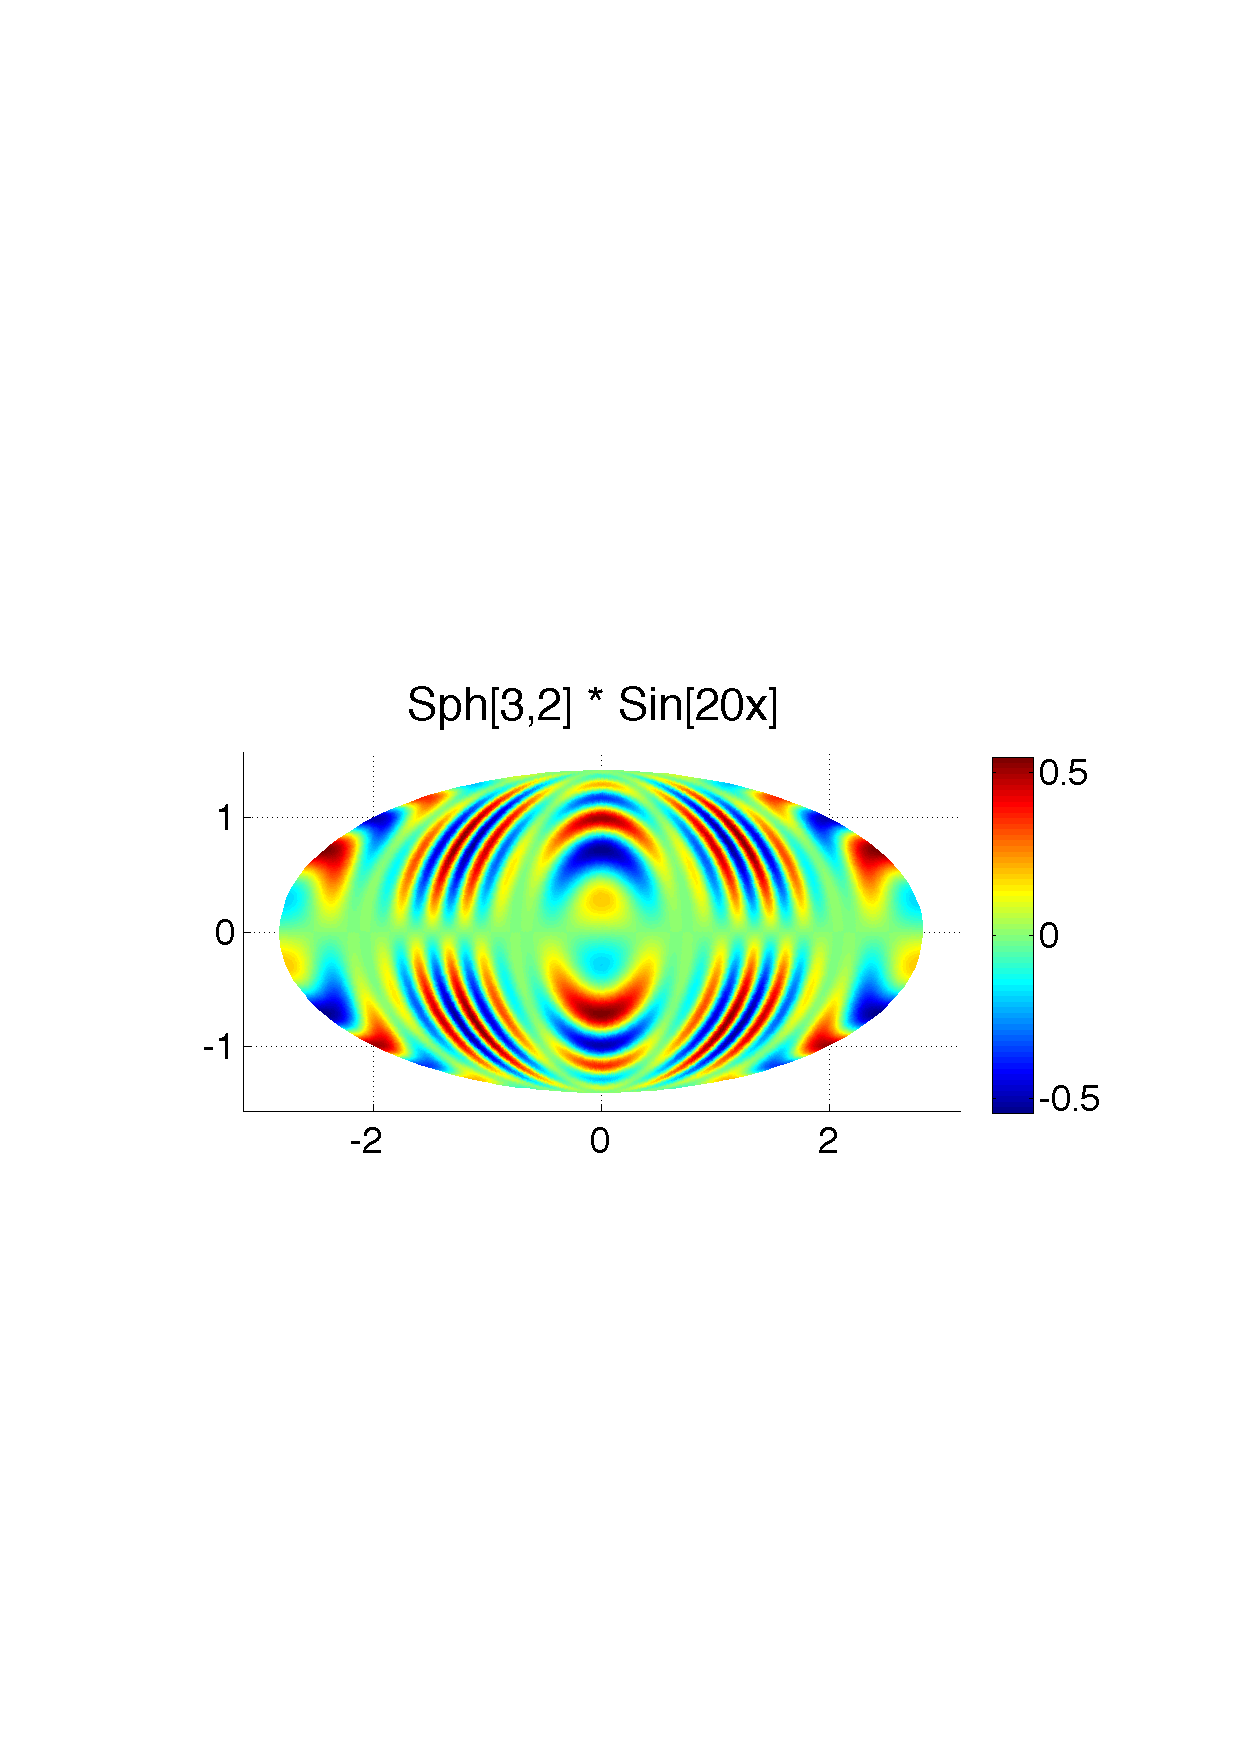
\includegraphics[width=1.0\textwidth]{figures/chapter2/compare_weight_generation/xsfc_vs_xsfc_alt_on_sph32_times_sine_20x/sph32_times_sin20x.pdf}
	\caption{Manufactured test function: \\  $f(\vx) = Y_{3}^{2}(\vx)\sin(20x)$.  }
	\end{subfigure}
	\begin{subfigure}[b]{0.425\textwidth}
	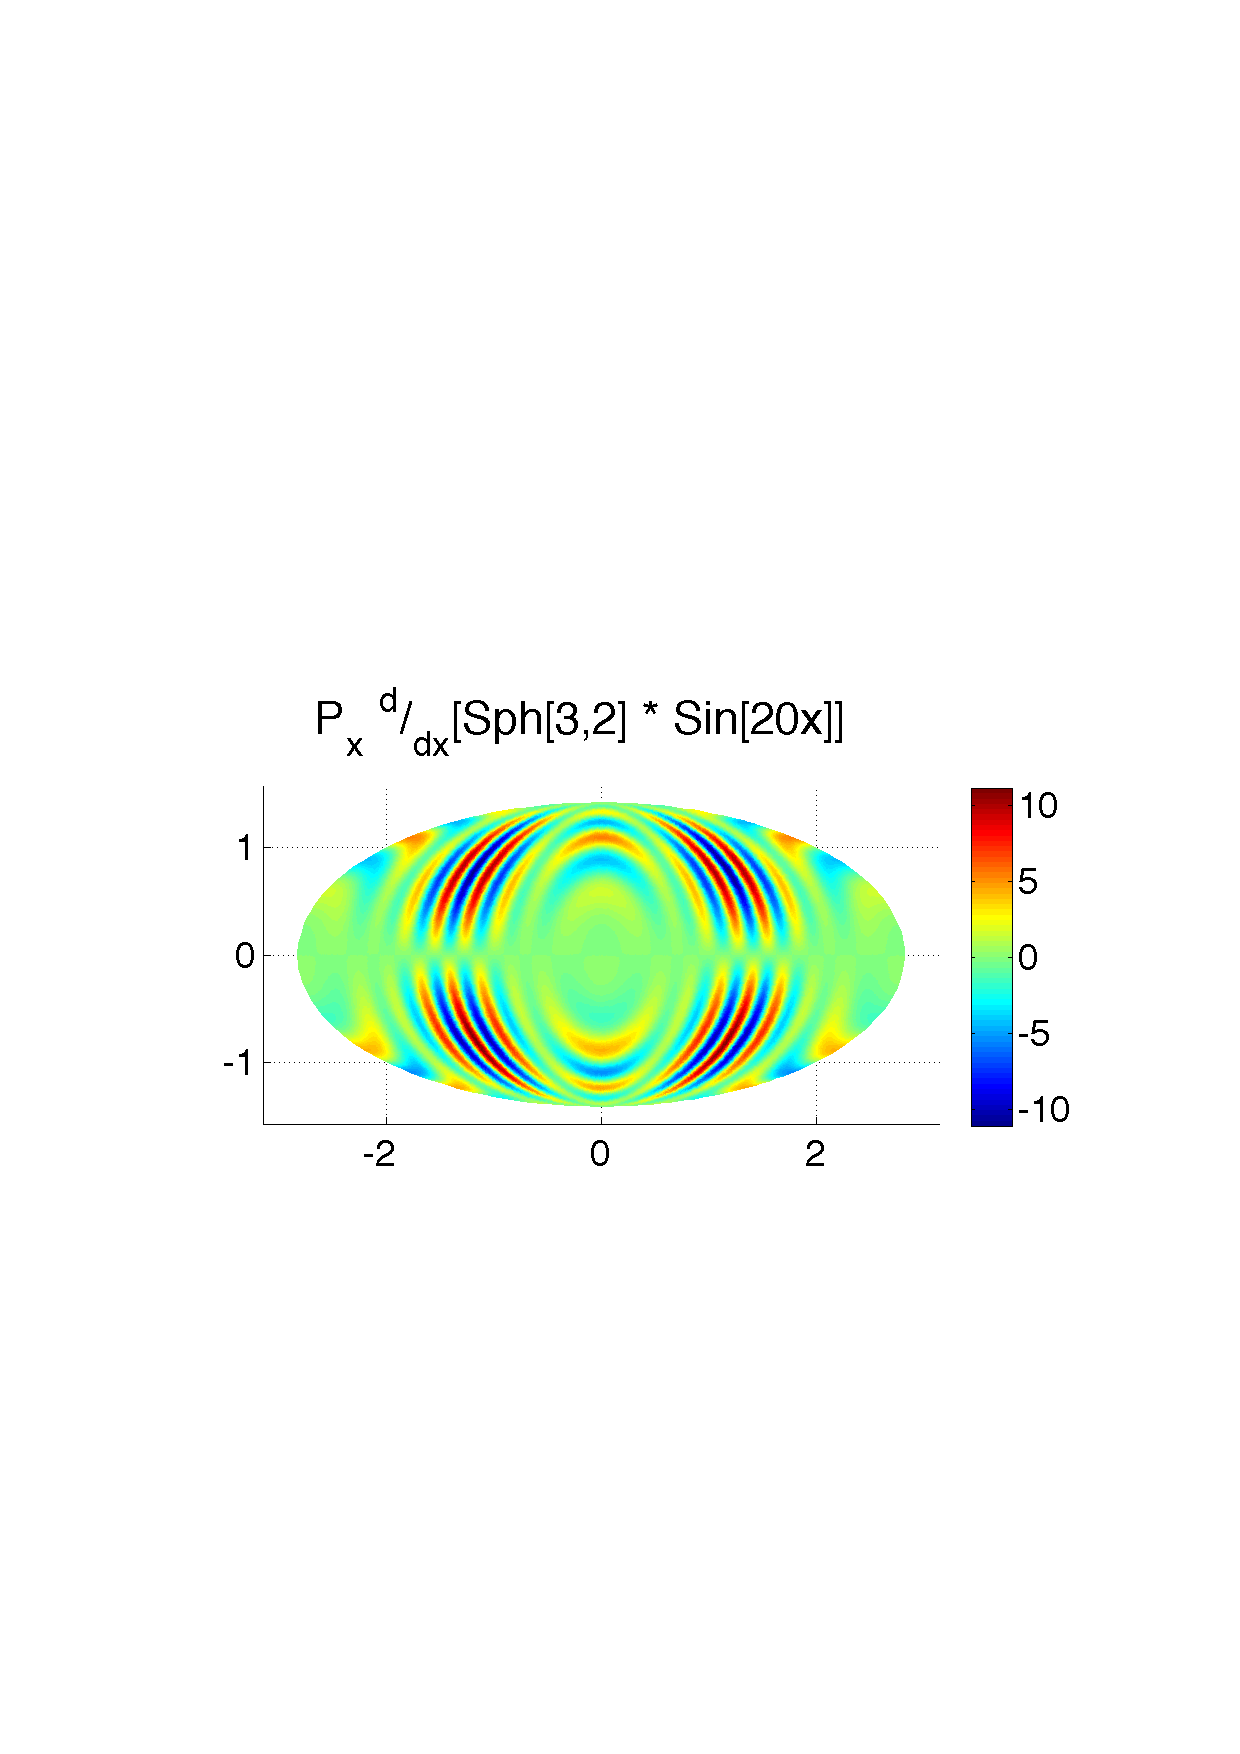
\includegraphics[width=1.0\textwidth]{figures/chapter2/compare_weight_generation/xsfc_vs_xsfc_alt_on_sph32_times_sine_20x/pdx_sph32_times_sin20x.pdf}
	\caption{$x$-component of the projected gradient: 
	$\mathbf{p}_{x} \cdot \nabla f(\vx)$.  }
	\end{subfigure}
	
	\begin{subfigure}[b]{0.425\textwidth}
	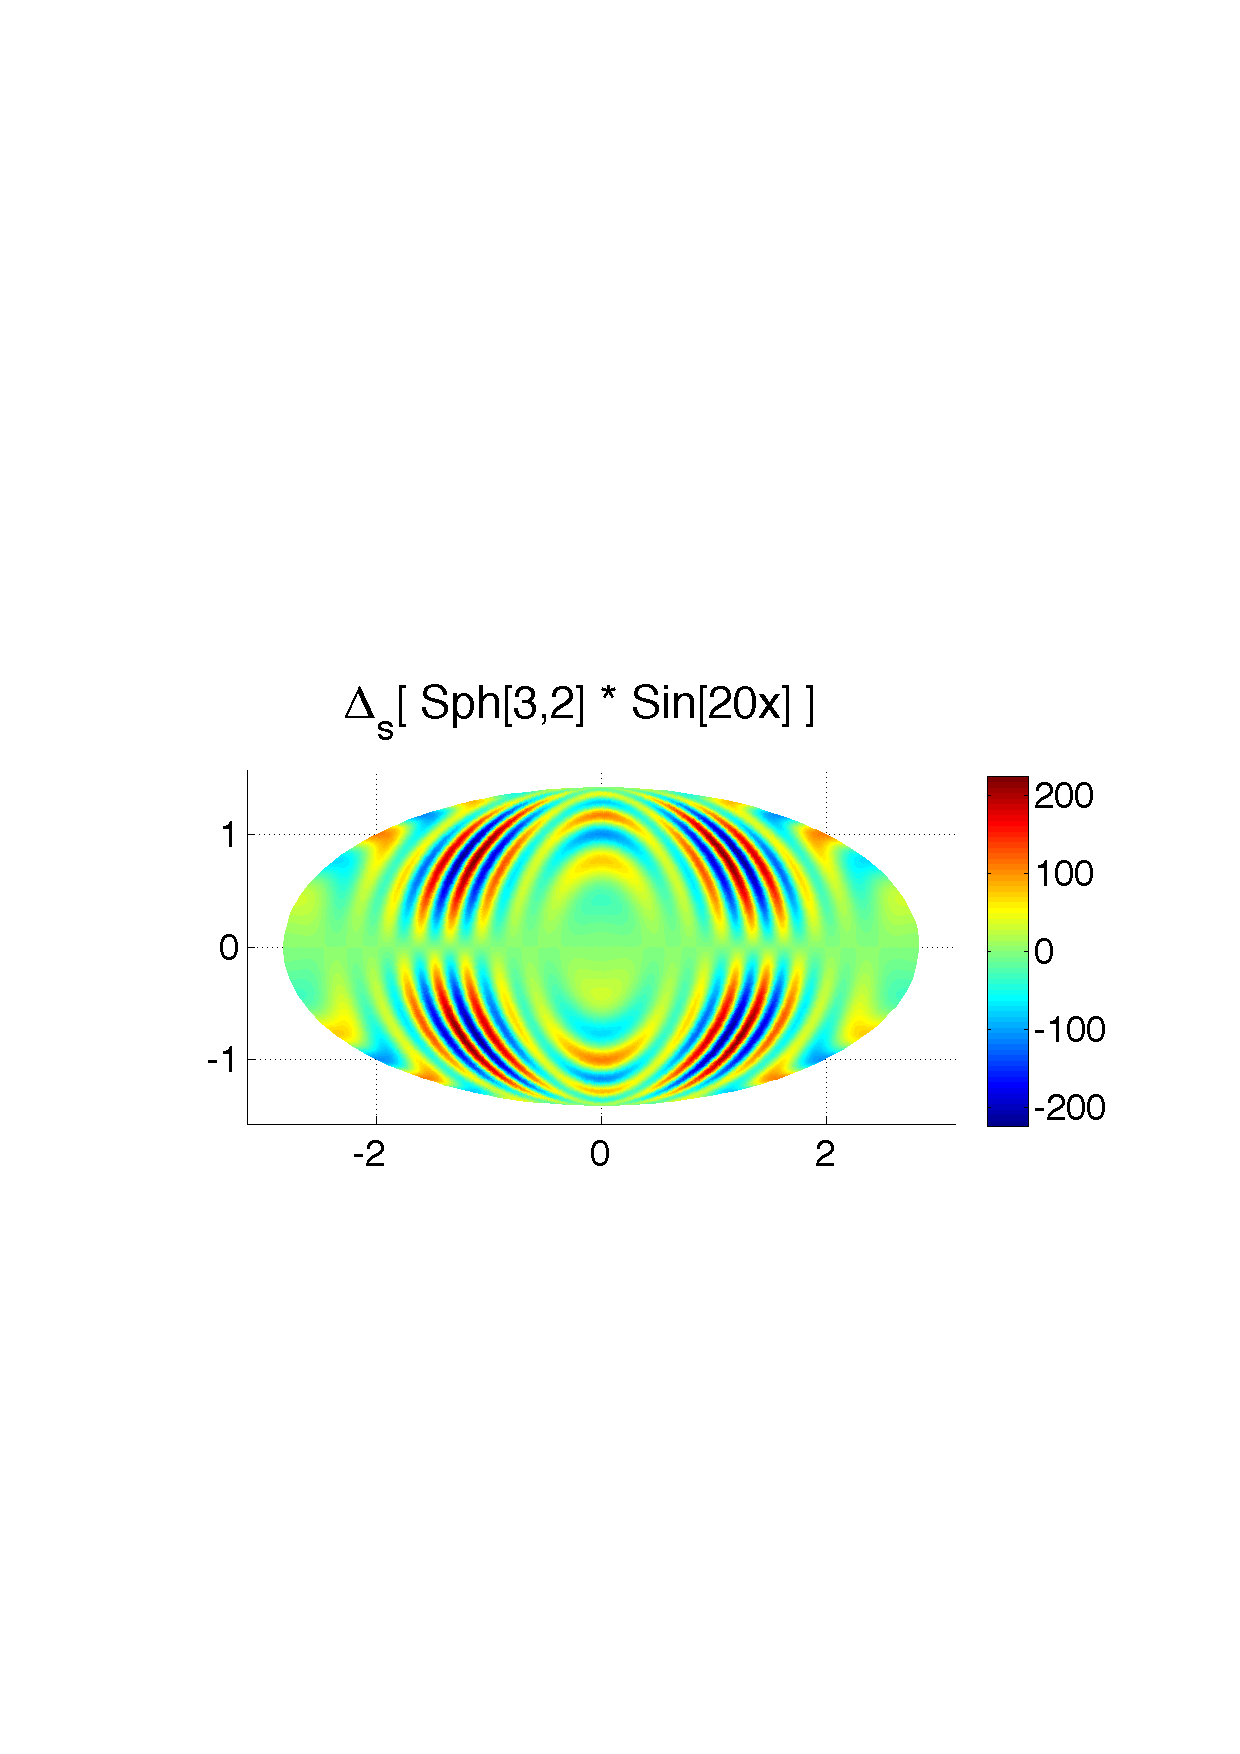
\includegraphics[width=1.0\textwidth]{figures/chapter2/compare_weight_generation/lsfc_vs_px_grad_dot_px_grad/lsfc_sph32_times_sin20x.pdf}
	\caption{Surface Laplacian: $\LaplaceBeltrami f(\vx)$.  }
	\end{subfigure}
	\caption{Test function and its projected $x$ derivatives. }
\end{figure}


\begin{figure}[htbp]
	\centering
	\begin{subfigure}[b]{0.425\textwidth}
	\includegraphics[width=1.0\textwidth]{figures/chapter2/compare_weight_generation/lsfc_vs_px_grad_dot_px_grad/direct_rel_l2_error.pdf}
	\caption{$\LaplaceBeltrami$ of }
		\end{subfigure}
	\begin{subfigure}[b]{0.425\textwidth}
\includegraphics[width=1.0\textwidth]{figures/chapter2/compare_weight_generation/xsfc_vs_xsfc_alt_on_sph32/direct_rel_l2_error.pdf}
	\end{subfigure}
	\begin{subfigure}[b]{0.425\textwidth}
\includegraphics[width=1.0\textwidth]{figures/chapter2/compare_weight_generation/xsfc_vs_xsfc_alt_on_sph32_times_sine_20x/direct_rel_l2_error.pdf}
	\end{subfigure}
	\caption{Relative $\ell_{2}$ error in differentiation.}
\end{figure}


\begin{figure}[htbp]
	\centering
	\begin{subfigure}[b]{0.425\textwidth}
	\includegraphics[width=1.0\textwidth]{figures/chapter2/compare_weight_generation/lsfc_vs_px_grad_dot_px_grad/diff_of_rel_l2_errors.pdf}
	\end{subfigure}
	\begin{subfigure}[b]{0.425\textwidth}
	\includegraphics[width=1.0\textwidth]{figures/chapter2/compare_weight_generation/xsfc_vs_xsfc_alt_on_sph32/diff_of_rel_l2_errors.pdf}
	\end{subfigure}
	\begin{subfigure}[b]{0.425\textwidth}
	\includegraphics[width=1.0\textwidth]{figures/chapter2/compare_weight_generation/xsfc_vs_xsfc_alt_on_sph32_times_sine_20x/diff_of_rel_l2_errors.pdf}
	\end{subfigure}
	\caption{Signed differences of relative $\ell_{2}$ errors in differentiation between Direct and Indirect weights.}
\end{figure}


\begin{figure}[htbp]
	\centering
	\begin{subfigure}[b]{0.425\textwidth}
	\includegraphics[width=1.0\textwidth]{figures/chapter2/compare_weight_generation/lsfc_vs_px_grad_dot_px_grad/abs_diff_of_rel_l2_errors.pdf}
		\end{subfigure}
	\begin{subfigure}[b]{0.425\textwidth}
	\includegraphics[width=1.0\textwidth]{figures/chapter2/compare_weight_generation/xsfc_vs_xsfc_alt_on_sph32_times_sine_20x/abs_diff_of_rel_l2_errors.pdf}
	\end{subfigure}
		\caption{Absolute differences of relative $\ell_{2}$ errors in differentiation between Direct and Indirect weights.}
\end{figure}

\begin{figure}[htbp]
\centering
\includegraphics[width=0.425\textwidth]{figures/chapter2/compare_weight_generation/xsfc_vs_xsfc_alt_on_sph32/condest_dm_xsfc.pdf}
\caption{Condition number estimates (condest) of direct $\mathbf{p}_{x}\nabla$ differentiation matrix}
\end{figure}
\section{Conclusions}

Although it is clear the indirect method functions well compared to the direct method, we must consider its usefulness. Typically, weights are computed only as necessary for the PDE. If the PDE is on the sphere, then directly computing the $\mathbf{P}\nabla$ operator would be most efficient for both memory and computation. However, one could imagine a scenario such as a 3-D spherical shell domain with physics on the boundaries that must be constrained to the surface, while the interior requires only an unprojected $\nabla$ operator. In such cases, by simply computing for the $\nabla$ operator, we assemble all necessary operators with minimal loss of accuracy and significant savings ($3Nn$ doubles) in storage. 

\authnote{Plot file size of matrix market file to give an idea of how much memory is saved by cutting out operators} 

With $N=1e6$ nodes and stencil size $n=101$, the matrix market file for weights is approximately 1.6 GB on disk. For a GPU with only 6 GB of global memory space available, it is worthwhile to consider possibilities for memory conservation. 


\authnote{Check to see $\nabla \cdot \nabla$ accuracy for heat equation.} 


% The BibTeX bibliography/references section.  View the file
% 'myrefs.bib' to get a feel for what these entries may look like.
% By using the optional \nocite{*} line, every entry in 'myrefs.bib'
% will be inserted into the bibliography.  Otherwise, only entries
% that have been cited with \cite{key} somewhere in the text will
% be included.
%\nocite{*}
% Or individually reference papers you want to include without citation: 
%\nocite{Vuduc2005}

\bibliographystyle{plain}
\bibliography{merged_references}

%\begin{biosketch}

Evan Bollig was born on the 6th of June, 1983, and grew up in the sleepy town of Sun Prairie, WI. He completed his Bachelor studies at the University of Minnesota--Twin Cities in 2006 with dual degrees in Computer Science and German Studies. 

In 2009, Evan was awarded a Master's Degree in Computational Science from the Department of Scientific Computing at Florida State University with a thesis titled, ``Centroidal Voronoi Tessellation of Manifolds using the GPU". As a Master's student, Evan worked as both a graduate research and teaching assistant in the Department of Scientific Computing.

During the summer of 2009, Evan was one of 11 participants in the Summer Internship in Parallel Computational Science (SIParCS) program at the National Center for Atmospheric Research (NCAR). The following year he returned to NCAR for a second internship; this time with Dr. Natasha Flyer in the Institute for Mathematics Applied to Geosciences (IMAGe) division. In 2011, he was invited to return a third time as a graduate student visitor for an extended collaboration with Dr. Flyer between June 2011 and February 2012. 

Evan was briefly employed as a Software Engineer by the Tallahassee, FL branch of Homes.com from August to December 2012. 

Presently, Evan lives in Saint Paul, MN, and works as a research associate for the University of Minnesota Supercomputing Institute (since December 2012). 


\end{biosketch}

\end{document}
